% Options for packages loaded elsewhere
\PassOptionsToPackage{unicode}{hyperref}
\PassOptionsToPackage{hyphens}{url}
%
\documentclass[
]{book}
\usepackage{amsmath,amssymb}
\usepackage{lmodern}
\usepackage{iftex}
\ifPDFTeX
  \usepackage[T1]{fontenc}
  \usepackage[utf8]{inputenc}
  \usepackage{textcomp} % provide euro and other symbols
\else % if luatex or xetex
  \usepackage{unicode-math}
  \defaultfontfeatures{Scale=MatchLowercase}
  \defaultfontfeatures[\rmfamily]{Ligatures=TeX,Scale=1}
\fi
% Use upquote if available, for straight quotes in verbatim environments
\IfFileExists{upquote.sty}{\usepackage{upquote}}{}
\IfFileExists{microtype.sty}{% use microtype if available
  \usepackage[]{microtype}
  \UseMicrotypeSet[protrusion]{basicmath} % disable protrusion for tt fonts
}{}
\makeatletter
\@ifundefined{KOMAClassName}{% if non-KOMA class
  \IfFileExists{parskip.sty}{%
    \usepackage{parskip}
  }{% else
    \setlength{\parindent}{0pt}
    \setlength{\parskip}{6pt plus 2pt minus 1pt}}
}{% if KOMA class
  \KOMAoptions{parskip=half}}
\makeatother
\usepackage{xcolor}
\IfFileExists{xurl.sty}{\usepackage{xurl}}{} % add URL line breaks if available
\IfFileExists{bookmark.sty}{\usepackage{bookmark}}{\usepackage{hyperref}}
\hypersetup{
  pdftitle={We R Under Way: A Data Science Portfolio},
  pdfauthor={Kaydee S. Barker},
  hidelinks,
  pdfcreator={LaTeX via pandoc}}
\urlstyle{same} % disable monospaced font for URLs
\usepackage{color}
\usepackage{fancyvrb}
\newcommand{\VerbBar}{|}
\newcommand{\VERB}{\Verb[commandchars=\\\{\}]}
\DefineVerbatimEnvironment{Highlighting}{Verbatim}{commandchars=\\\{\}}
% Add ',fontsize=\small' for more characters per line
\usepackage{framed}
\definecolor{shadecolor}{RGB}{248,248,248}
\newenvironment{Shaded}{\begin{snugshade}}{\end{snugshade}}
\newcommand{\AlertTok}[1]{\textcolor[rgb]{0.94,0.16,0.16}{#1}}
\newcommand{\AnnotationTok}[1]{\textcolor[rgb]{0.56,0.35,0.01}{\textbf{\textit{#1}}}}
\newcommand{\AttributeTok}[1]{\textcolor[rgb]{0.77,0.63,0.00}{#1}}
\newcommand{\BaseNTok}[1]{\textcolor[rgb]{0.00,0.00,0.81}{#1}}
\newcommand{\BuiltInTok}[1]{#1}
\newcommand{\CharTok}[1]{\textcolor[rgb]{0.31,0.60,0.02}{#1}}
\newcommand{\CommentTok}[1]{\textcolor[rgb]{0.56,0.35,0.01}{\textit{#1}}}
\newcommand{\CommentVarTok}[1]{\textcolor[rgb]{0.56,0.35,0.01}{\textbf{\textit{#1}}}}
\newcommand{\ConstantTok}[1]{\textcolor[rgb]{0.00,0.00,0.00}{#1}}
\newcommand{\ControlFlowTok}[1]{\textcolor[rgb]{0.13,0.29,0.53}{\textbf{#1}}}
\newcommand{\DataTypeTok}[1]{\textcolor[rgb]{0.13,0.29,0.53}{#1}}
\newcommand{\DecValTok}[1]{\textcolor[rgb]{0.00,0.00,0.81}{#1}}
\newcommand{\DocumentationTok}[1]{\textcolor[rgb]{0.56,0.35,0.01}{\textbf{\textit{#1}}}}
\newcommand{\ErrorTok}[1]{\textcolor[rgb]{0.64,0.00,0.00}{\textbf{#1}}}
\newcommand{\ExtensionTok}[1]{#1}
\newcommand{\FloatTok}[1]{\textcolor[rgb]{0.00,0.00,0.81}{#1}}
\newcommand{\FunctionTok}[1]{\textcolor[rgb]{0.00,0.00,0.00}{#1}}
\newcommand{\ImportTok}[1]{#1}
\newcommand{\InformationTok}[1]{\textcolor[rgb]{0.56,0.35,0.01}{\textbf{\textit{#1}}}}
\newcommand{\KeywordTok}[1]{\textcolor[rgb]{0.13,0.29,0.53}{\textbf{#1}}}
\newcommand{\NormalTok}[1]{#1}
\newcommand{\OperatorTok}[1]{\textcolor[rgb]{0.81,0.36,0.00}{\textbf{#1}}}
\newcommand{\OtherTok}[1]{\textcolor[rgb]{0.56,0.35,0.01}{#1}}
\newcommand{\PreprocessorTok}[1]{\textcolor[rgb]{0.56,0.35,0.01}{\textit{#1}}}
\newcommand{\RegionMarkerTok}[1]{#1}
\newcommand{\SpecialCharTok}[1]{\textcolor[rgb]{0.00,0.00,0.00}{#1}}
\newcommand{\SpecialStringTok}[1]{\textcolor[rgb]{0.31,0.60,0.02}{#1}}
\newcommand{\StringTok}[1]{\textcolor[rgb]{0.31,0.60,0.02}{#1}}
\newcommand{\VariableTok}[1]{\textcolor[rgb]{0.00,0.00,0.00}{#1}}
\newcommand{\VerbatimStringTok}[1]{\textcolor[rgb]{0.31,0.60,0.02}{#1}}
\newcommand{\WarningTok}[1]{\textcolor[rgb]{0.56,0.35,0.01}{\textbf{\textit{#1}}}}
\usepackage{longtable,booktabs,array}
\usepackage{calc} % for calculating minipage widths
% Correct order of tables after \paragraph or \subparagraph
\usepackage{etoolbox}
\makeatletter
\patchcmd\longtable{\par}{\if@noskipsec\mbox{}\fi\par}{}{}
\makeatother
% Allow footnotes in longtable head/foot
\IfFileExists{footnotehyper.sty}{\usepackage{footnotehyper}}{\usepackage{footnote}}
\makesavenoteenv{longtable}
\usepackage{graphicx}
\makeatletter
\def\maxwidth{\ifdim\Gin@nat@width>\linewidth\linewidth\else\Gin@nat@width\fi}
\def\maxheight{\ifdim\Gin@nat@height>\textheight\textheight\else\Gin@nat@height\fi}
\makeatother
% Scale images if necessary, so that they will not overflow the page
% margins by default, and it is still possible to overwrite the defaults
% using explicit options in \includegraphics[width, height, ...]{}
\setkeys{Gin}{width=\maxwidth,height=\maxheight,keepaspectratio}
% Set default figure placement to htbp
\makeatletter
\def\fps@figure{htbp}
\makeatother
\setlength{\emergencystretch}{3em} % prevent overfull lines
\providecommand{\tightlist}{%
  \setlength{\itemsep}{0pt}\setlength{\parskip}{0pt}}
\setcounter{secnumdepth}{5}
\ifLuaTeX
  \usepackage{selnolig}  % disable illegal ligatures
\fi
\usepackage[]{natbib}
\bibliographystyle{apalike}

\title{We R Under Way: A Data Science Portfolio}
\author{Kaydee S. Barker}
\date{Last compiled on 20 May, 2022}

\begin{document}
\maketitle

{
\setcounter{tocdepth}{1}
\tableofcontents
}
Writing and code by Kaydee Barker, assignments by Dr.~Ross and Dr.~Mueller (SOCR 580A7), Dr.~Lefsky (ESS 330) of Colorado State University. Data cited within chapters.

\hypertarget{intro}{%
\chapter{Introduction}\label{intro}}

\begin{quote}
``There are two kinds of data scientists: 1) Those who can extrapolate from incomplete data.''
\end{quote}

I began my foray into R in the spring of 2020, first teaching myself some basic syntax and then using it for statistical analysis on my research projects as an undergraduate researcher at Colorado State University (CSU). With the help of my research mentors and many amazing people of the internet, I was able to fumble my way forward and learn a number of techniques to analyze and visualize data in R. I have since been building on my R and data science skills, including with the help of two key courses at CSU: ``Quantitative Reasoning for Ecosystem Science'' (ESS 330) and ``Introduction to Environmental Data Science'' (SOCR 580A7). Since I can't yet publish data from my research projects, this portfolio is constructed of public data examples, primarily from my coursework in those two courses. Its purpose is a) to serve as a reference for myself and others learning to use R for environmental analyses, and b) to demonstrate my current R knowledge to advisors and colleagues.

\hypertarget{interactive-graphing-discharge-of-the-poudre-river}{%
\chapter{Interactive Graphing: Discharge of the Poudre River}\label{interactive-graphing-discharge-of-the-poudre-river}}

\begin{quote}
``Someone asked me to name two structures that hold water. I was like, `well\ldots{} damn!'\,''
\end{quote}

This assignment used a unique package of R Markdown (dygraphs) in order to create an interactive chart.

Data and assignment provided by Dr.~Matthew Ross and Dr.~Nathan Mueller of Colorado State University.

\hypertarget{background-on-the-poudre-river}{%
\section{Background on the Poudre River}\label{background-on-the-poudre-river}}

\href{https://edits.nationalmap.gov/apps/gaz-domestic/public/summary/205018}{Cache La Poudre River} is an important watershed that supports \textbf{agriculture, industry, recreation, and residential needs} on the Front Range of Colorado. It also provides for cottonwood forest, shrub, and grassland ecosystems that support \href{http://poudretrail.org/habitat-wildlife/\#fish}{wildlife} from the mountains down to the prairies. The unique \textbf{biodiversity} and \textbf{history} of the Cache La Poudre watershed are valued widely; 45 miles along the Poudre are encompassed in a \href{https://www.nps.gov/places/cache-la-poudre-river-national-heritage-area.htm}{National Heritage Area}.
The history of Cache La Poudre is linked to the \emph{history of the West}, because its banks supported the first major \href{https://www-jstor-org.ezproxy2.library.colostate.edu/stable/pdf/1821074.pdf}{irrigation-based agricultural settlement} of its kind in 1870, which would soon spread through the Arid West.

\hypertarget{interactive-discharge-chart}{%
\section{Interactive Discharge Chart}\label{interactive-discharge-chart}}

\begin{Shaded}
\begin{Highlighting}[]
\NormalTok{q }\OtherTok{\textless{}{-}} \FunctionTok{readNWISdv}\NormalTok{(}\AttributeTok{siteNumbers =} \StringTok{\textquotesingle{}06752260\textquotesingle{}}\NormalTok{,}
                \AttributeTok{parameterCd =} \StringTok{\textquotesingle{}00060\textquotesingle{}}\NormalTok{,}
                \AttributeTok{startDate =} \StringTok{\textquotesingle{}2017{-}01{-}01\textquotesingle{}}\NormalTok{,}
                \AttributeTok{endDate =} \StringTok{\textquotesingle{}2022{-}01{-}01\textquotesingle{}}\NormalTok{) }\SpecialCharTok{\%\textgreater{}\%}
  \FunctionTok{rename}\NormalTok{(}\AttributeTok{q =} \StringTok{\textquotesingle{}X\_00060\_00003\textquotesingle{}}\NormalTok{)}

\NormalTok{q\_xts }\OtherTok{\textless{}{-}} \FunctionTok{xts}\NormalTok{(q}\SpecialCharTok{$}\NormalTok{q, }\AttributeTok{order.by =}\NormalTok{ q}\SpecialCharTok{$}\NormalTok{Date)}

\FunctionTok{dygraph}\NormalTok{(q\_xts) }\SpecialCharTok{\%\textgreater{}\%}
  \FunctionTok{dyAxis}\NormalTok{(}\StringTok{"y"}\NormalTok{, }\AttributeTok{label =} \StringTok{"Discharge (cfs)"}\NormalTok{) }\SpecialCharTok{\%\textgreater{}\%}
  \FunctionTok{dyOptions}\NormalTok{(}\AttributeTok{drawPoints =} \ConstantTok{TRUE}\NormalTok{, }\AttributeTok{pointSize =} \DecValTok{2}\NormalTok{)}
\end{Highlighting}
\end{Shaded}

\begin{verbatim}
## PhantomJS not found. You can install it with webshot::install_phantomjs(). If it is installed, please make sure the phantomjs executable can be found via the PATH variable.
\end{verbatim}

\label{fig:interactive}Discharge of the Poudre River in cubic feet per second from January 2017 to December 2021.

\hypertarget{looking-at-effects-of-fire-on-vegetation}{%
\chapter{Looking at Effects of Fire on Vegetation}\label{looking-at-effects-of-fire-on-vegetation}}

\begin{quote}
``What happens when a wildfire tells you a joke? You get burned!''
\end{quote}

This assignment demonstrates the benefit of visualizing data to see potential correlations.

Data and assignment provided by Dr.~Matthew Ross and Dr.~Nathan Mueller of Colorado State University.

\hypertarget{introduction}{%
\section{Introduction}\label{introduction}}

The Hayman Fire, started by arsen in summer of 2002, was the largest wildfire in Colorado history until the 2020 wildfire season. It burned a large area of over 138 thousand acres between the Kenosha Mountains and Pikes Peak, affecting wildlife and causing water quality concerns for the Front Range populations through damage to watersheds that contribute to the South Platte River.

\hypertarget{what-is-the-correlation-between-ndvi-and-ndmi}{%
\section{What is the correlation between NDVI and NDMI?}\label{what-is-the-correlation-between-ndvi-and-ndmi}}

The Normalized Difference Vegetation Index (NDVI) is positively correlated with the Normalized Difference Moisture Index (NDMI). In everyday terms, NDVI indicates plant health as shown by how well leaves reflect near infrared and red light, while NDMI represents plant water content and is calculated from near infrared and short-wave infrared reflectance values (\href{https://www.agricolus.com/en/vegetation-indices-ndvi-ndmi/}{Agricolus, 2018}). These values can also tell us about how much vegetative cover there is at a given site, with the lowest NDVI (\textless0.1) and NDMI (\textless-0.8) values indicating bare soil.

Not surprisingly, the plot below shows that canopy cover is greatly decreased for the burned site compared to the unburned site.

\begin{Shaded}
\begin{Highlighting}[]
\CommentTok{\#ggplot of wide set in summer}
\NormalTok{full\_wide }\SpecialCharTok{\%\textgreater{}\%}
  \FunctionTok{filter}\NormalTok{(month }\SpecialCharTok{\%in\%} \FunctionTok{c}\NormalTok{(}\DecValTok{6}\NormalTok{,}\DecValTok{7}\NormalTok{,}\DecValTok{8}\NormalTok{,}\DecValTok{9}\NormalTok{,}\DecValTok{10}\NormalTok{)) }\SpecialCharTok{\%\textgreater{}\%}
  \FunctionTok{filter}\NormalTok{(year }\SpecialCharTok{\textgreater{}=} \DecValTok{2002}\NormalTok{) }\SpecialCharTok{\%\textgreater{}\%}
\FunctionTok{ggplot}\NormalTok{(., }\FunctionTok{aes}\NormalTok{(}\AttributeTok{x=}\NormalTok{ndmi,}\AttributeTok{y=}\NormalTok{ndvi, }\AttributeTok{color=}\NormalTok{treatment)) }\SpecialCharTok{+} 
  \FunctionTok{geom\_point}\NormalTok{(}\AttributeTok{shape=}\DecValTok{1}\NormalTok{) }\SpecialCharTok{+} 
  \FunctionTok{xlab}\NormalTok{(}\StringTok{"NDMI"}\NormalTok{) }\SpecialCharTok{+} \FunctionTok{ylab}\NormalTok{(}\StringTok{"NDVI"}\NormalTok{) }\SpecialCharTok{+}
  \FunctionTok{ggtitle}\NormalTok{(}\StringTok{"Burned vs. Unburned Vegetation"}\NormalTok{) }\SpecialCharTok{+}
  \FunctionTok{theme\_few}\NormalTok{(}\AttributeTok{base\_size =} \DecValTok{16}\NormalTok{) }\SpecialCharTok{+}
  \FunctionTok{scale\_color\_brewer}\NormalTok{(}\AttributeTok{palette =} \StringTok{"Set2"}\NormalTok{) }\SpecialCharTok{+}
  \FunctionTok{theme}\NormalTok{(}\AttributeTok{panel.grid.major=}\FunctionTok{element\_blank}\NormalTok{(), }\AttributeTok{panel.grid.minor=}\FunctionTok{element\_blank}\NormalTok{(), }\AttributeTok{legend.position=}\StringTok{"bottom"}\NormalTok{)}
\end{Highlighting}
\end{Shaded}

\begin{figure}
\centering
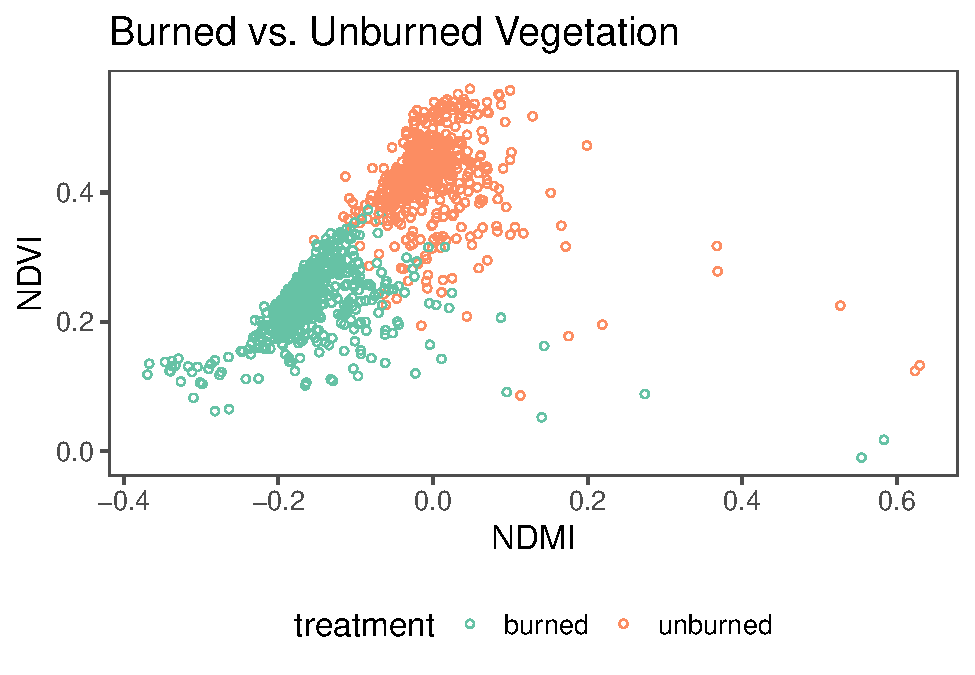
\includegraphics{Rportfolio-bookdown_files/figure-latex/unnamed-chunk-2-1.pdf}
\caption{\label{fig:unnamed-chunk-2}NDVI and NDMI values from 2002 to 2019 in Colorado sites that were burned (teal) or left unburned (orange) during the Hayman Fire.}
\end{figure}

As may be expected, vegetative growth (NDVI) is positively associated with the previous winter's snowfall, as shown in the plot below.

\begin{Shaded}
\begin{Highlighting}[]
\CommentTok{\#ggplot winter NDSI to summer NDVI}
\FunctionTok{ggplot}\NormalTok{(ndvi\_ndsi, }\FunctionTok{aes}\NormalTok{(}\AttributeTok{x =}\NormalTok{ mean\_NDVI, }\AttributeTok{y =}\NormalTok{ mean\_NDSI)) }\SpecialCharTok{+}
  \FunctionTok{geom\_point}\NormalTok{(}\AttributeTok{fill =} \StringTok{"blue"}\NormalTok{, }
             \AttributeTok{shape =} \DecValTok{21}\NormalTok{, }
             \AttributeTok{size =} \DecValTok{2}\NormalTok{) }\SpecialCharTok{+}
  \FunctionTok{geom\_smooth}\NormalTok{(}\AttributeTok{method =} \StringTok{"lm"}\NormalTok{,}
              \AttributeTok{se =} \ConstantTok{TRUE}\NormalTok{,}
              \AttributeTok{lty =} \DecValTok{1}\NormalTok{,}
              \AttributeTok{color =} \StringTok{"black"}\NormalTok{,}
              \AttributeTok{fill =} \StringTok{"lightgrey"}\NormalTok{,}
              \AttributeTok{size =} \DecValTok{1}\NormalTok{) }\SpecialCharTok{+}
  \FunctionTok{xlab}\NormalTok{(}\StringTok{"Mean NDSI"}\NormalTok{) }\SpecialCharTok{+} \FunctionTok{ylab}\NormalTok{(}\StringTok{"Mean NDVI"}\NormalTok{) }\SpecialCharTok{+}
  \FunctionTok{ggtitle}\NormalTok{(}\StringTok{"Winter NDSI vs. Summer NDVI"}\NormalTok{) }\SpecialCharTok{+}
  \FunctionTok{theme\_few}\NormalTok{(}\AttributeTok{base\_size =} \DecValTok{16}\NormalTok{) }\SpecialCharTok{+}
  \FunctionTok{scale\_y\_continuous}\NormalTok{(}\AttributeTok{breaks =} \FunctionTok{pretty}\NormalTok{(}\FunctionTok{c}\NormalTok{(}\SpecialCharTok{{-}}\FloatTok{0.4}\NormalTok{,}\FloatTok{0.5}\NormalTok{), }\AttributeTok{n =} \DecValTok{4}\NormalTok{)) }\SpecialCharTok{+}
  \FunctionTok{scale\_x\_continuous}\NormalTok{(}\AttributeTok{breaks =} \FunctionTok{pretty}\NormalTok{(}\FunctionTok{c}\NormalTok{(}\FloatTok{0.2}\NormalTok{,}\FloatTok{0.5}\NormalTok{), }\AttributeTok{n =} \DecValTok{6}\NormalTok{)) }\SpecialCharTok{+}
  \FunctionTok{theme}\NormalTok{(}\AttributeTok{panel.grid.major=}\FunctionTok{element\_blank}\NormalTok{(), }\AttributeTok{panel.grid.minor=}\FunctionTok{element\_blank}\NormalTok{(), }\AttributeTok{legend.position=}\StringTok{"bottom"}\NormalTok{)}
\end{Highlighting}
\end{Shaded}

\begin{verbatim}
## `geom_smooth()` using formula 'y ~ x'
\end{verbatim}

\begin{figure}
\centering
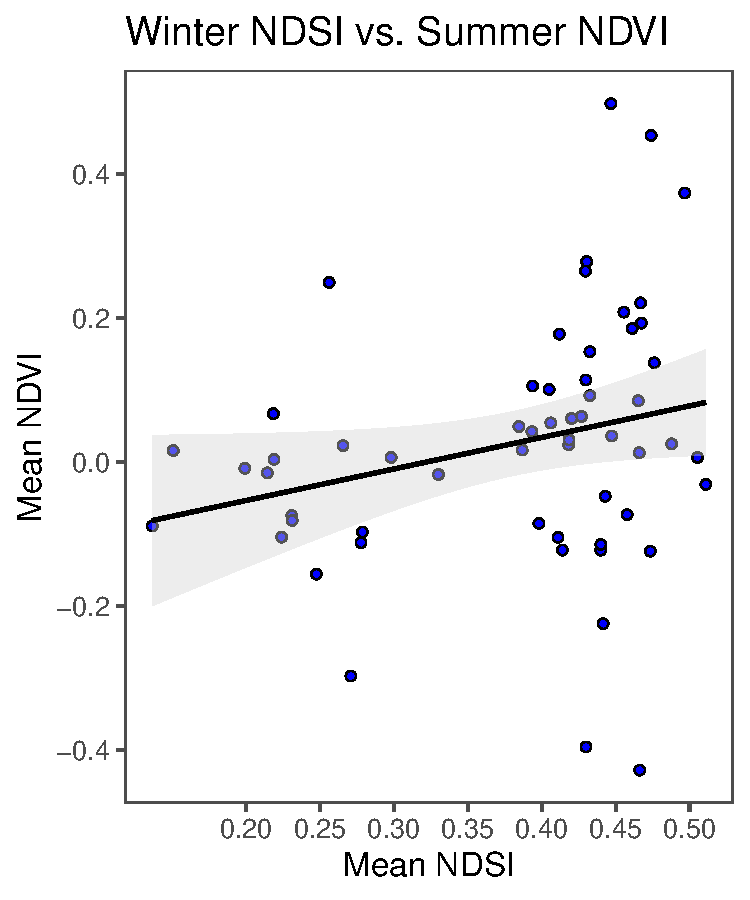
\includegraphics{Rportfolio-bookdown_files/figure-latex/unnamed-chunk-3-1.pdf}
\caption{\label{fig:unnamed-chunk-3}Linear models for mean summer NDVI and mean winter NDSI for pre- and post-burn and burned and unburned sites.}
\end{figure}

\hypertarget{what-month-is-the-greenest-month-on-average}{%
\section{What month is the greenest month on average?}\label{what-month-is-the-greenest-month-on-average}}

If we plot monthly means of NDVI, we can see that the greenest month in Colorado is August.

\begin{Shaded}
\begin{Highlighting}[]
\CommentTok{\#ggplot of monthly means}
\NormalTok{monthly\_sum }\SpecialCharTok{\%\textgreater{}\%}
  \FunctionTok{filter}\NormalTok{(data }\SpecialCharTok{==} \StringTok{"ndvi"}\NormalTok{) }\SpecialCharTok{\%\textgreater{}\%}
  \FunctionTok{mutate\_at}\NormalTok{(}\FunctionTok{vars}\NormalTok{(month), }\FunctionTok{funs}\NormalTok{(factor)) }\SpecialCharTok{\%\textgreater{}\%}
\FunctionTok{ggplot}\NormalTok{(., }\FunctionTok{aes}\NormalTok{(}\AttributeTok{x=}\NormalTok{month, }\AttributeTok{y=}\NormalTok{value\_mean, }\AttributeTok{fill=}\NormalTok{month)) }\SpecialCharTok{+} 
  \FunctionTok{geom\_bar}\NormalTok{(}\AttributeTok{stat =} \StringTok{"identity"}\NormalTok{, }\AttributeTok{width =} \FloatTok{0.7}\NormalTok{, }\AttributeTok{position =} \StringTok{"dodge"}\NormalTok{) }\SpecialCharTok{+}
  \FunctionTok{geom\_errorbar}\NormalTok{(}\FunctionTok{aes}\NormalTok{(}\AttributeTok{ymin=}\NormalTok{value\_mean}\SpecialCharTok{{-}}\NormalTok{value\_std.error, }\AttributeTok{ymax=}\NormalTok{value\_mean}\SpecialCharTok{+}\NormalTok{value\_std.error), }
                \AttributeTok{colour =} \StringTok{"black"}\NormalTok{, }\AttributeTok{width =} \FloatTok{0.7}\NormalTok{, }\AttributeTok{position =} \StringTok{"dodge"}\NormalTok{) }\SpecialCharTok{+}
  \FunctionTok{scale\_x\_discrete}\NormalTok{(}\AttributeTok{labels=}\FunctionTok{c}\NormalTok{(}\StringTok{"5"}\OtherTok{=}\StringTok{"May"}\NormalTok{, }\StringTok{"6"}\OtherTok{=}\StringTok{"June"}\NormalTok{, }\StringTok{"7"}\OtherTok{=}\StringTok{"Jul."}\NormalTok{, }\StringTok{"8"}\OtherTok{=}\StringTok{"Aug."}\NormalTok{, }\StringTok{"9"}\OtherTok{=}\StringTok{"Sept."}\NormalTok{)) }\SpecialCharTok{+}
  \FunctionTok{xlab}\NormalTok{(}\StringTok{"Month"}\NormalTok{) }\SpecialCharTok{+}  \FunctionTok{ylab}\NormalTok{(}\StringTok{"NDVI"}\NormalTok{) }\SpecialCharTok{+}
  \FunctionTok{ggtitle}\NormalTok{(}\StringTok{"Average NDVI per Month"}\NormalTok{) }\SpecialCharTok{+}
  \FunctionTok{theme\_few}\NormalTok{() }\SpecialCharTok{+}
  \FunctionTok{scale\_fill\_brewer}\NormalTok{(}\AttributeTok{palette =} \StringTok{"Greens"}\NormalTok{) }\SpecialCharTok{+}
  \FunctionTok{theme}\NormalTok{(}\AttributeTok{panel.grid.major=}\FunctionTok{element\_blank}\NormalTok{(), }
        \AttributeTok{panel.grid.minor=}\FunctionTok{element\_blank}\NormalTok{(), }\AttributeTok{legend.position=}\StringTok{"none"}\NormalTok{)}
\end{Highlighting}
\end{Shaded}

\begin{figure}
\centering
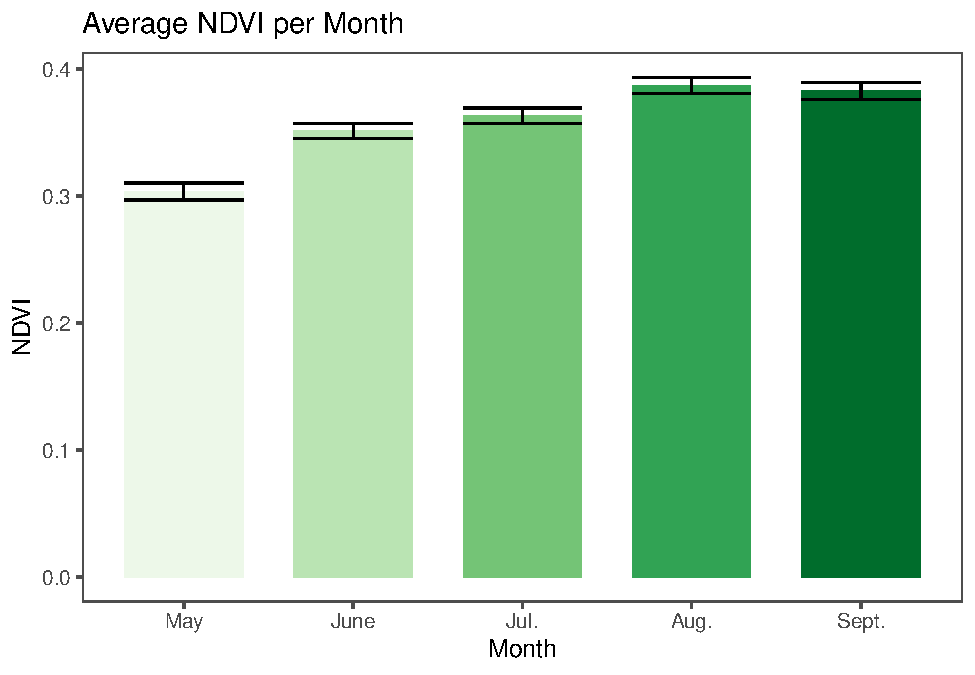
\includegraphics{Rportfolio-bookdown_files/figure-latex/unnamed-chunk-4-1.pdf}
\caption{\label{fig:unnamed-chunk-4}Mean NDVI and standard error per summer month across sites from 1984 to 2019.}
\end{figure}

\hypertarget{what-month-is-the-snowiest-on-average}{%
\section{What month is the snowiest on average?}\label{what-month-is-the-snowiest-on-average}}

If we plot the NDSI means for the winter months, we can see that the highest snowfall is January.

\begin{Shaded}
\begin{Highlighting}[]
\CommentTok{\# Change ordering manually and make month into factor}
\NormalTok{monthly\_win}\SpecialCharTok{$}\NormalTok{month }\OtherTok{\textless{}{-}} \FunctionTok{factor}\NormalTok{(monthly\_win}\SpecialCharTok{$}\NormalTok{month,   }
                  \AttributeTok{levels =} \FunctionTok{c}\NormalTok{(}\StringTok{"11"}\NormalTok{,}\StringTok{"12"}\NormalTok{, }\StringTok{"1"}\NormalTok{, }\StringTok{"2"}\NormalTok{, }\StringTok{"3"}\NormalTok{))}

\NormalTok{monthly\_win }\SpecialCharTok{\%\textgreater{}\%}
  \FunctionTok{filter}\NormalTok{(data }\SpecialCharTok{==} \StringTok{"ndsi"}\NormalTok{) }\SpecialCharTok{\%\textgreater{}\%}
\FunctionTok{ggplot}\NormalTok{(., }\FunctionTok{aes}\NormalTok{(}\AttributeTok{x=}\NormalTok{month,}\AttributeTok{y=}\NormalTok{value\_mean, }\AttributeTok{fill=}\NormalTok{month)) }\SpecialCharTok{+} 
  \FunctionTok{geom\_bar}\NormalTok{(}\AttributeTok{stat =} \StringTok{"identity"}\NormalTok{, }\AttributeTok{width =} \FloatTok{0.7}\NormalTok{, }\AttributeTok{position =} \StringTok{"dodge"}\NormalTok{) }\SpecialCharTok{+}
  \FunctionTok{geom\_errorbar}\NormalTok{(}\FunctionTok{aes}\NormalTok{(}\AttributeTok{ymin=}\NormalTok{value\_mean}\SpecialCharTok{{-}}\NormalTok{value\_std.error, }\AttributeTok{ymax=}\NormalTok{value\_mean}\SpecialCharTok{+}\NormalTok{value\_std.error), }
                \AttributeTok{colour =} \StringTok{"black"}\NormalTok{, }\AttributeTok{width =} \FloatTok{0.7}\NormalTok{, }\AttributeTok{position =} \StringTok{"dodge"}\NormalTok{) }\SpecialCharTok{+}
  \FunctionTok{scale\_x\_discrete}\NormalTok{(}\AttributeTok{labels=}\FunctionTok{c}\NormalTok{(}\StringTok{"11"}\OtherTok{=}\StringTok{"Nov."}\NormalTok{, }\StringTok{"12"}\OtherTok{=}\StringTok{"Dec"}\NormalTok{, }\StringTok{"1"}\OtherTok{=}\StringTok{"Jan."}\NormalTok{, }\StringTok{"2"}\OtherTok{=}\StringTok{"Feb."}\NormalTok{, }
                            \StringTok{"3"}\OtherTok{=}\StringTok{"Mar."}\NormalTok{)) }\SpecialCharTok{+}
  \FunctionTok{xlab}\NormalTok{(}\StringTok{"Month"}\NormalTok{) }\SpecialCharTok{+}  \FunctionTok{ylab}\NormalTok{(}\StringTok{"NDSI"}\NormalTok{) }\SpecialCharTok{+}
  \FunctionTok{ggtitle}\NormalTok{(}\StringTok{"Average NDSI per Month"}\NormalTok{) }\SpecialCharTok{+}
  \FunctionTok{theme\_few}\NormalTok{() }\SpecialCharTok{+}
  \FunctionTok{scale\_fill\_brewer}\NormalTok{(}\AttributeTok{palette =} \StringTok{"Purples"}\NormalTok{) }\SpecialCharTok{+}
  \FunctionTok{theme}\NormalTok{(}\AttributeTok{panel.grid.major=}\FunctionTok{element\_blank}\NormalTok{(), }\AttributeTok{panel.grid.minor=}\FunctionTok{element\_blank}\NormalTok{(), }
        \AttributeTok{legend.position=}\StringTok{"none"}\NormalTok{)}
\end{Highlighting}
\end{Shaded}

\begin{figure}
\centering
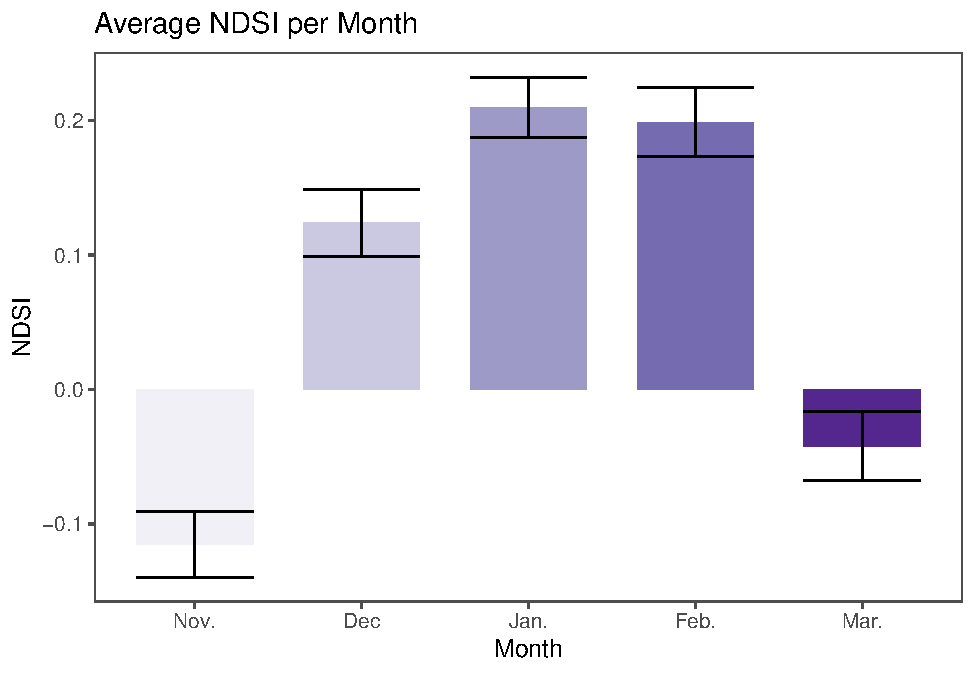
\includegraphics{Rportfolio-bookdown_files/figure-latex/unnamed-chunk-5-1.pdf}
\caption{\label{fig:unnamed-chunk-5}Mean NDSI and standard error per winter month across sites from 1984 to 2019.}
\end{figure}

\hypertarget{fire-effects-on-fish-populations}{%
\chapter{Fire Effects on Fish Populations}\label{fire-effects-on-fish-populations}}

Wildfires don't only impact vegetation, but a wide variety of abiotic and biotic elements of the ecosystem. In this assignment, I looked at how fish in the Cache La Poudre Watershed were impacted by the High Park Fire in 2012.

Data and assignment provided by Dr.~Michael Lefsky of Colorado State University.

\hypertarget{pre-versus-post-fire-fish-length-and-mass}{%
\section{Pre versus post fire fish length and mass}\label{pre-versus-post-fire-fish-length-and-mass}}

\begin{Shaded}
\begin{Highlighting}[]
\CommentTok{\#summarize fishdata\_R by time (another way to do this without subsets)}
\FunctionTok{summary}\NormalTok{(fishdata\_4R[fishdata\_4R}\SpecialCharTok{$}\NormalTok{time}\SpecialCharTok{==}\StringTok{"pre{-}fire"}\NormalTok{,])}
\end{Highlighting}
\end{Shaded}

\begin{verbatim}
##      time             capture_id       length_cm         mass_g   
##  Length:100         Min.   :  1.00   Min.   : 5.00   Min.   : 66  
##  Class :character   1st Qu.: 25.75   1st Qu.:15.00   1st Qu.:132  
##  Mode  :character   Median : 50.50   Median :18.00   Median :151  
##                     Mean   : 50.50   Mean   :19.16   Mean   :154  
##                     3rd Qu.: 75.25   3rd Qu.:23.00   3rd Qu.:182  
##                     Max.   :100.00   Max.   :32.00   Max.   :252
\end{verbatim}

\begin{Shaded}
\begin{Highlighting}[]
\FunctionTok{summary}\NormalTok{(fishdata\_4R[fishdata\_4R}\SpecialCharTok{$}\NormalTok{time}\SpecialCharTok{==}\StringTok{"post{-}fire"}\NormalTok{,])}
\end{Highlighting}
\end{Shaded}

\begin{verbatim}
##      time             capture_id   length_cm         mass_g     
##  Length:97          Min.   : 1   Min.   : 5.00   Min.   : 45.0  
##  Class :character   1st Qu.:25   1st Qu.:15.00   1st Qu.: 89.0  
##  Mode  :character   Median :49   Median :20.00   Median :113.0  
##                     Mean   :49   Mean   :19.76   Mean   :107.9  
##                     3rd Qu.:73   3rd Qu.:25.00   3rd Qu.:126.0  
##                     Max.   :97   Max.   :38.00   Max.   :157.0
\end{verbatim}

\begin{Shaded}
\begin{Highlighting}[]
\CommentTok{\# create function to run statistics}
\NormalTok{lab\_stats }\OtherTok{\textless{}{-}} \ControlFlowTok{function}\NormalTok{(x) }\FunctionTok{c}\NormalTok{(}\FunctionTok{sd}\NormalTok{(x),}\FunctionTok{sd}\NormalTok{(x)}\SpecialCharTok{\^{}}\DecValTok{2}\NormalTok{,}\FunctionTok{sd}\NormalTok{(x)}\SpecialCharTok{/}\FunctionTok{sqrt}\NormalTok{(}\FunctionTok{length}\NormalTok{(x))) }\CommentTok{\#calculate standard deviation, variance, standard error. Return as vector}

\CommentTok{\#Pre{-}fire statistics}
\FunctionTok{lab\_stats}\NormalTok{(fishdata\_4R[fishdata\_4R}\SpecialCharTok{$}\NormalTok{time}\SpecialCharTok{==}\StringTok{"pre{-}fire"}\NormalTok{,]}\SpecialCharTok{$}\NormalTok{length\_cm) }\CommentTok{\#fish length}
\end{Highlighting}
\end{Shaded}

\begin{verbatim}
## [1]  6.2145479 38.6206061  0.6214548
\end{verbatim}

\begin{Shaded}
\begin{Highlighting}[]
\FunctionTok{lab\_stats}\NormalTok{(fishdata\_4R[fishdata\_4R}\SpecialCharTok{$}\NormalTok{time}\SpecialCharTok{==}\StringTok{"pre{-}fire"}\NormalTok{,]}\SpecialCharTok{$}\NormalTok{mass\_g) }\CommentTok{\#fish mass}
\end{Highlighting}
\end{Shaded}

\begin{verbatim}
## [1]   36.277409 1316.050404    3.627741
\end{verbatim}

\begin{Shaded}
\begin{Highlighting}[]
\CommentTok{\#Post{-}fire statistics}
\FunctionTok{lab\_stats}\NormalTok{(fishdata\_4R[fishdata\_4R}\SpecialCharTok{$}\NormalTok{time}\SpecialCharTok{==}\StringTok{"post{-}fire"}\NormalTok{,]}\SpecialCharTok{$}\NormalTok{length\_cm) }\CommentTok{\#fish length}
\end{Highlighting}
\end{Shaded}

\begin{verbatim}
## [1]  7.0574624 49.8077749  0.7165767
\end{verbatim}

\begin{Shaded}
\begin{Highlighting}[]
\FunctionTok{lab\_stats}\NormalTok{(fishdata\_4R[fishdata\_4R}\SpecialCharTok{$}\NormalTok{time}\SpecialCharTok{==}\StringTok{"post{-}fire"}\NormalTok{,]}\SpecialCharTok{$}\NormalTok{mass\_g) }\CommentTok{\#fish mass}
\end{Highlighting}
\end{Shaded}

\begin{verbatim}
## [1]  26.894853 723.333119   2.730759
\end{verbatim}

\begin{Shaded}
\begin{Highlighting}[]
\CommentTok{\# 1{-}way ANOVA on pre{-} vs. post{-}fire mass and length}
\FunctionTok{summary}\NormalTok{(}\FunctionTok{aov}\NormalTok{(fishdata\_4R}\SpecialCharTok{$}\NormalTok{length\_cm}\SpecialCharTok{\textasciitilde{}}\NormalTok{fishdata\_4R}\SpecialCharTok{$}\NormalTok{time)) }\CommentTok{\#ANOVA for fish length pre vs. post fire}
\end{Highlighting}
\end{Shaded}

\begin{verbatim}
##                   Df Sum Sq Mean Sq F value Pr(>F)
## fishdata_4R$time   1     18   17.90   0.406  0.525
## Residuals        195   8605   44.13
\end{verbatim}

\begin{Shaded}
\begin{Highlighting}[]
\FunctionTok{summary}\NormalTok{(}\FunctionTok{aov}\NormalTok{(fishdata\_4R}\SpecialCharTok{$}\NormalTok{mass\_g}\SpecialCharTok{\textasciitilde{}}\NormalTok{fishdata\_4R}\SpecialCharTok{$}\NormalTok{time)) }\CommentTok{\#ANOVA for fish mass pre vs. post fire}
\end{Highlighting}
\end{Shaded}

\begin{verbatim}
##                   Df Sum Sq Mean Sq F value Pr(>F)    
## fishdata_4R$time   1 104798  104798   102.3 <2e-16 ***
## Residuals        195 199729    1024                   
## ---
## Signif. codes:  0 '***' 0.001 '**' 0.01 '*' 0.05 '.' 0.1 ' ' 1
\end{verbatim}

\begin{Shaded}
\begin{Highlighting}[]
\CommentTok{\# Make a 2 x 2 matrix of histograms for pre{-} and post{-}fire mass and length}
\FunctionTok{par}\NormalTok{(}\AttributeTok{mfrow=}\FunctionTok{c}\NormalTok{(}\DecValTok{2}\NormalTok{,}\DecValTok{2}\NormalTok{)) }\CommentTok{\#tell R how I want figures arranged}

\CommentTok{\#Pre{-}fire histograms}
\FunctionTok{hist}\NormalTok{(fishdata\_4R[fishdata\_4R}\SpecialCharTok{$}\NormalTok{time }\SpecialCharTok{==} \StringTok{"pre{-}fire"}\NormalTok{,]}\SpecialCharTok{$}\NormalTok{length\_cm,}\AttributeTok{main=}\StringTok{"Pre{-}fire length (cm)"}\NormalTok{,}\AttributeTok{xlab=}\StringTok{"Length (cm)"}\NormalTok{) }\CommentTok{\#fish length}
\FunctionTok{hist}\NormalTok{(fishdata\_4R[fishdata\_4R}\SpecialCharTok{$}\NormalTok{time }\SpecialCharTok{==} \StringTok{"pre{-}fire"}\NormalTok{,]}\SpecialCharTok{$}\NormalTok{mass\_g,}\AttributeTok{main=}\StringTok{"Pre{-}fire mass (g)"}\NormalTok{,}\AttributeTok{xlab=}\StringTok{"Mass (g)"}\NormalTok{) }\CommentTok{\#fish mass}

\CommentTok{\#Post{-}fire histograms}
\FunctionTok{hist}\NormalTok{(fishdata\_4R[fishdata\_4R}\SpecialCharTok{$}\NormalTok{time }\SpecialCharTok{==} \StringTok{"post{-}fire"}\NormalTok{,]}\SpecialCharTok{$}\NormalTok{length\_cm,}\AttributeTok{main=}\StringTok{"Post{-}fire length (cm)"}\NormalTok{,}\AttributeTok{xlab=}\StringTok{"Length (cm)"}\NormalTok{) }\CommentTok{\#fish length}
\FunctionTok{hist}\NormalTok{(fishdata\_4R[fishdata\_4R}\SpecialCharTok{$}\NormalTok{time }\SpecialCharTok{==} \StringTok{"post{-}fire"}\NormalTok{,]}\SpecialCharTok{$}\NormalTok{mass\_g,}\AttributeTok{main=}\StringTok{"Post{-}fire mass (g)"}\NormalTok{,}\AttributeTok{xlab=}\StringTok{"Mass (g)"}\NormalTok{) }\CommentTok{\#fish mass}
\end{Highlighting}
\end{Shaded}

\begin{figure}
\centering
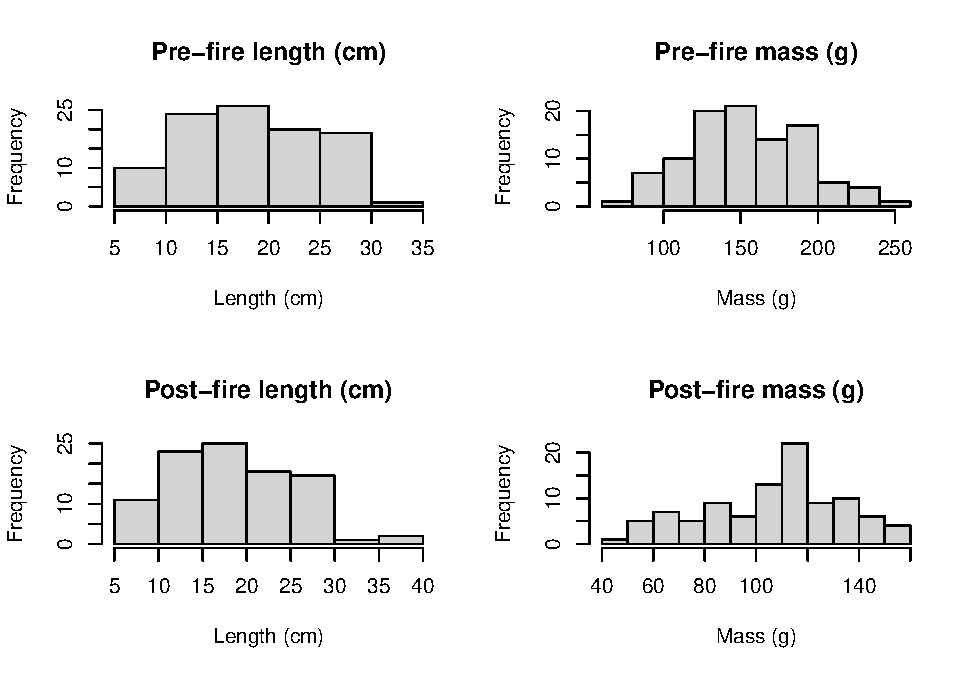
\includegraphics{Rportfolio-bookdown_files/figure-latex/unnamed-chunk-8-1.pdf}
\caption{\label{fig:unnamed-chunk-8}Histograms showing frequency of various lengths in centimeters and masses in grams of fish in in Cache La Poudre Watershed in 2012 before the High Park Fire (Pre-fire) and in 2013 after the High Park Fire (Post-fire).}
\end{figure}

\begin{Shaded}
\begin{Highlighting}[]
\CommentTok{\# Make a 2 x 2 matrix of histograms for pre{-} and post{-}fire mass and length}
\FunctionTok{par}\NormalTok{(}\AttributeTok{mfrow=}\FunctionTok{c}\NormalTok{(}\DecValTok{2}\NormalTok{,}\DecValTok{2}\NormalTok{)) }\CommentTok{\#tell R how I want figures arranged}

\CommentTok{\# Make two boxplots side by side}
\FunctionTok{par}\NormalTok{(}\AttributeTok{mfrow=}\FunctionTok{c}\NormalTok{(}\DecValTok{1}\NormalTok{,}\DecValTok{2}\NormalTok{)) }\CommentTok{\#tell R I want two plots}
\FunctionTok{boxplot}\NormalTok{(fishdata\_4R}\SpecialCharTok{$}\NormalTok{length\_cm}\SpecialCharTok{\textasciitilde{}}\NormalTok{fishdata\_4R}\SpecialCharTok{$}\NormalTok{time, }\AttributeTok{main=}\StringTok{"Length (cm)"}\NormalTok{,}\AttributeTok{ylab =} \StringTok{"Frequency"}\NormalTok{,}\AttributeTok{xlab=}\StringTok{"Time"}\NormalTok{) }\CommentTok{\#length fre and post fire}
\FunctionTok{boxplot}\NormalTok{(fishdata\_4R}\SpecialCharTok{$}\NormalTok{mass\_g}\SpecialCharTok{\textasciitilde{}}\NormalTok{fishdata\_4R}\SpecialCharTok{$}\NormalTok{time, }\AttributeTok{main=}\StringTok{"Mass (g)"}\NormalTok{,}\AttributeTok{ylab =} \StringTok{"Frequency"}\NormalTok{,}\AttributeTok{xlab=}\StringTok{"Time"}\NormalTok{) }\CommentTok{\#length fre and post fire}
\end{Highlighting}
\end{Shaded}

\begin{figure}
\centering
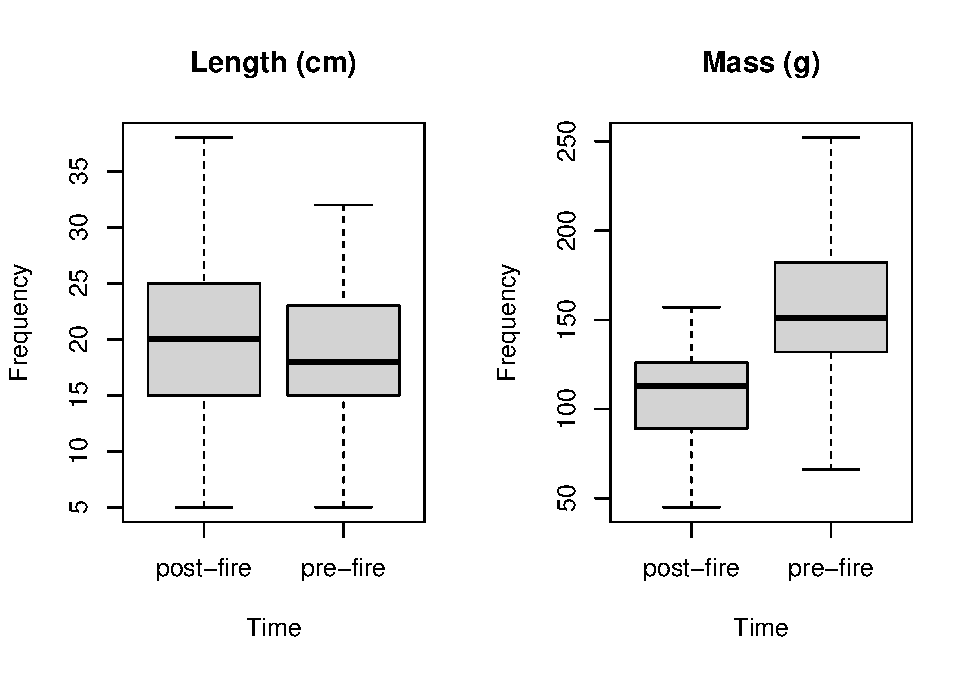
\includegraphics{Rportfolio-bookdown_files/figure-latex/unnamed-chunk-9-1.pdf}
\caption{\label{fig:unnamed-chunk-9}Boxplots for fish length in centimeters and mass in grams pre and post fire.}
\end{figure}

\begin{Shaded}
\begin{Highlighting}[]
\CommentTok{\# Reset setting for plots}
\FunctionTok{par}\NormalTok{(}\AttributeTok{mfrow=}\FunctionTok{c}\NormalTok{(}\DecValTok{1}\NormalTok{,}\DecValTok{1}\NormalTok{)) }\CommentTok{\#return to single plot}
\end{Highlighting}
\end{Shaded}

\hypertarget{linear-regression-of-fish-mass-vs.-length-for-before-and-after-the-fire}{%
\section{Linear regression of fish mass vs.~length for before and after the fire}\label{linear-regression-of-fish-mass-vs.-length-for-before-and-after-the-fire}}

\begin{Shaded}
\begin{Highlighting}[]
\CommentTok{\# Pre{-}fire}
\CommentTok{\# Scatterplot of length and mass where length is the independent variable and mass is the response variable}
\FunctionTok{plot}\NormalTok{(mass\_g }\SpecialCharTok{\textasciitilde{}}\NormalTok{ length\_cm, }\AttributeTok{data=}\NormalTok{fishdata\_4R[fishdata\_4R}\SpecialCharTok{$}\NormalTok{time}\SpecialCharTok{==}\StringTok{"pre{-}fire"}\NormalTok{,], }\AttributeTok{xlab=}\StringTok{"Length (cm)"}\NormalTok{, }\AttributeTok{ylab=}\StringTok{"Mass (g)"}\NormalTok{)}
\FunctionTok{title}\NormalTok{(}\StringTok{"Pre{-}fire Fish Mass vs. Length"}\NormalTok{)}

\CommentTok{\# Linear regression on mass vs.length}
\NormalTok{lm\_pre }\OtherTok{\textless{}{-}} \FunctionTok{lm}\NormalTok{(mass\_g }\SpecialCharTok{\textasciitilde{}}\NormalTok{ length\_cm,}\AttributeTok{data=}\NormalTok{fishdata\_4R[fishdata\_4R}\SpecialCharTok{$}\NormalTok{time}\SpecialCharTok{==}\StringTok{"pre{-}fire"}\NormalTok{,])}
\FunctionTok{abline}\NormalTok{(lm\_pre)  }\CommentTok{\#Adds the trendline to the regression scatterplot}
\end{Highlighting}
\end{Shaded}

\begin{figure}
\centering
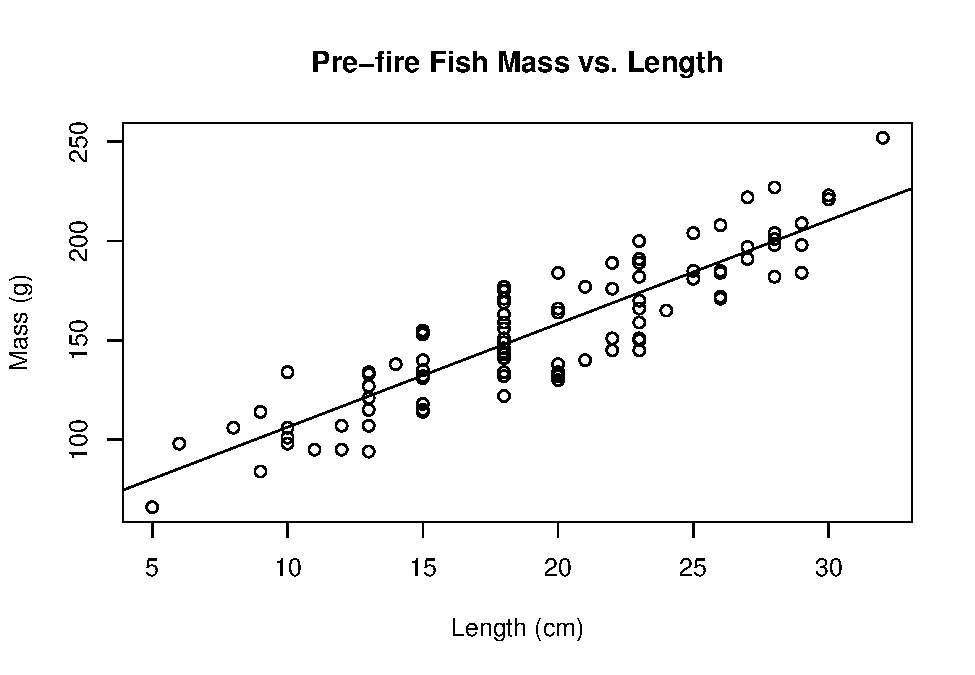
\includegraphics{Rportfolio-bookdown_files/figure-latex/unnamed-chunk-10-1.pdf}
\caption{\label{fig:unnamed-chunk-10}Scatterplot and linear regression line of fish length in centimeters versus fish mass in grams in Cache La Poudre in 2012 before the High Park Fire.}
\end{figure}

\begin{Shaded}
\begin{Highlighting}[]
\FunctionTok{summary}\NormalTok{(}\FunctionTok{aov}\NormalTok{(lm\_pre)) }\CommentTok{\#shows the results of the pre{-}fire linear regression ANOVA}
\end{Highlighting}
\end{Shaded}

\begin{verbatim}
##             Df Sum Sq Mean Sq F value Pr(>F)    
## length_cm    1 103690  103690     382 <2e-16 ***
## Residuals   98  26599     271                   
## ---
## Signif. codes:  0 '***' 0.001 '**' 0.01 '*' 0.05 '.' 0.1 ' ' 1
\end{verbatim}

\begin{Shaded}
\begin{Highlighting}[]
\FunctionTok{summary}\NormalTok{(lm\_pre) }\CommentTok{\#shows equation of the line, multiple R{-}squared value}
\end{Highlighting}
\end{Shaded}

\begin{verbatim}
## 
## Call:
## lm(formula = mass_g ~ length_cm, data = fishdata_4R[fishdata_4R$time == 
##     "pre-fire", ])
## 
## Residuals:
##     Min      1Q  Median      3Q     Max 
## -28.987 -14.472  -0.307  12.543  31.144 
## 
## Coefficients:
##             Estimate Std. Error t value Pr(>|t|)    
## (Intercept)  54.2113     5.3641   10.11   <2e-16 ***
## length_cm     5.2077     0.2664   19.55   <2e-16 ***
## ---
## Signif. codes:  0 '***' 0.001 '**' 0.01 '*' 0.05 '.' 0.1 ' ' 1
## 
## Residual standard error: 16.47 on 98 degrees of freedom
## Multiple R-squared:  0.7958, Adjusted R-squared:  0.7938 
## F-statistic:   382 on 1 and 98 DF,  p-value: < 2.2e-16
\end{verbatim}

\begin{Shaded}
\begin{Highlighting}[]
\CommentTok{\# Post{-}fire}
\CommentTok{\# Scatterplot of length and mass where length is the independent variable and mass is the response variable}
\FunctionTok{plot}\NormalTok{(mass\_g }\SpecialCharTok{\textasciitilde{}}\NormalTok{ length\_cm, }\AttributeTok{data=}\NormalTok{fishdata\_4R[fishdata\_4R}\SpecialCharTok{$}\NormalTok{time}\SpecialCharTok{==}\StringTok{"post{-}fire"}\NormalTok{,], }\AttributeTok{xlab=}\StringTok{"Length (cm)"}\NormalTok{, }\AttributeTok{ylab=}\StringTok{"Mass (g)"}\NormalTok{)}
\FunctionTok{title}\NormalTok{(}\StringTok{"Post{-}fire Fish Mass vs. Length"}\NormalTok{)}

\CommentTok{\# Linear regression on mass vs.length}
\NormalTok{lm\_post }\OtherTok{\textless{}{-}} \FunctionTok{lm}\NormalTok{(mass\_g }\SpecialCharTok{\textasciitilde{}}\NormalTok{ length\_cm,}\AttributeTok{data=}\NormalTok{fishdata\_4R[fishdata\_4R}\SpecialCharTok{$}\NormalTok{time}\SpecialCharTok{==}\StringTok{"post{-}fire"}\NormalTok{,])}
\FunctionTok{abline}\NormalTok{(lm\_post)  }\CommentTok{\#Adds the trendline to the regression scatterplot}
\end{Highlighting}
\end{Shaded}

\begin{figure}
\centering
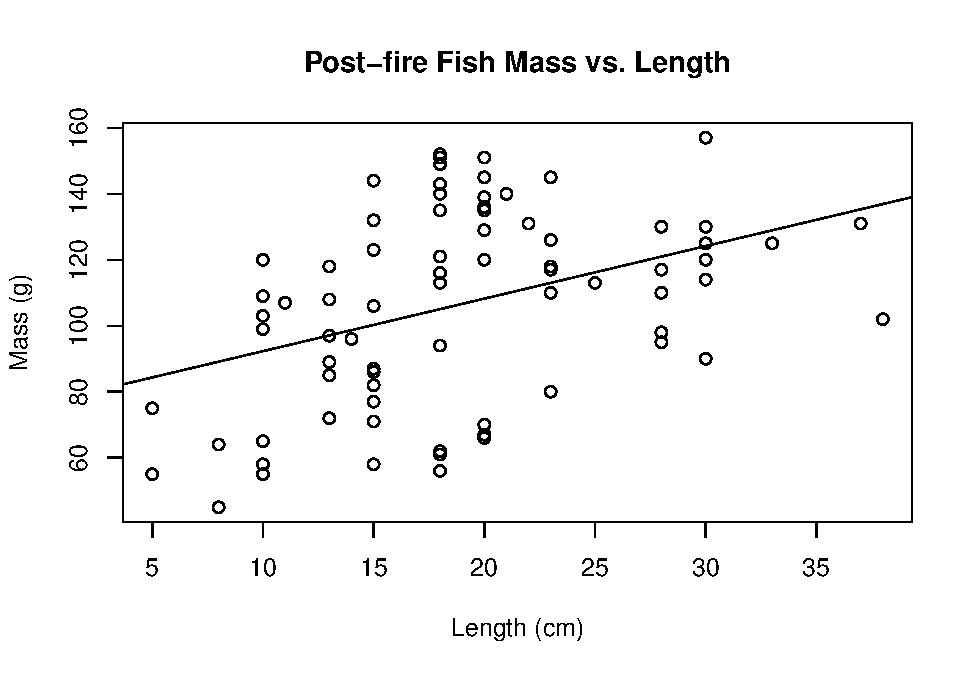
\includegraphics{Rportfolio-bookdown_files/figure-latex/unnamed-chunk-11-1.pdf}
\caption{\label{fig:unnamed-chunk-11}Scatterplot and linear regression line of fish length in centimeters versus fish mass in grams in Cache La Poudre in 2013 after the High Park Fire.}
\end{figure}

\begin{Shaded}
\begin{Highlighting}[]
\FunctionTok{summary}\NormalTok{(}\FunctionTok{aov}\NormalTok{(lm\_post)) }\CommentTok{\#shows the results of the pre{-}fire linear regression ANOVA}
\end{Highlighting}
\end{Shaded}

\begin{verbatim}
##             Df Sum Sq Mean Sq F value   Pr(>F)    
## length_cm    1  12126   12126    20.1 2.05e-05 ***
## Residuals   95  57313     603                     
## ---
## Signif. codes:  0 '***' 0.001 '**' 0.01 '*' 0.05 '.' 0.1 ' ' 1
\end{verbatim}

\begin{Shaded}
\begin{Highlighting}[]
\FunctionTok{summary}\NormalTok{(lm\_post) }\CommentTok{\#shows equation of the line, multiple R{-}squared value}
\end{Highlighting}
\end{Shaded}

\begin{verbatim}
## 
## Call:
## lm(formula = mass_g ~ length_cm, data = fishdata_4R[fishdata_4R$time == 
##     "post-fire", ])
## 
## Residuals:
##     Min      1Q  Median      3Q     Max 
## -49.048 -13.271  -3.011  19.582  46.952 
## 
## Coefficients:
##             Estimate Std. Error t value Pr(>|t|)    
## (Intercept)  76.3830     7.4498  10.253  < 2e-16 ***
## length_cm     1.5925     0.3552   4.483 2.05e-05 ***
## ---
## Signif. codes:  0 '***' 0.001 '**' 0.01 '*' 0.05 '.' 0.1 ' ' 1
## 
## Residual standard error: 24.56 on 95 degrees of freedom
## Multiple R-squared:  0.1746, Adjusted R-squared:  0.1659 
## F-statistic:  20.1 on 1 and 95 DF,  p-value: 2.054e-05
\end{verbatim}

\begin{Shaded}
\begin{Highlighting}[]
\CommentTok{\#Pre{-} and Post{-}Fire on same graph}

\CommentTok{\# First plot the pre{-}fire linear regression}
\CommentTok{\# ylim sets the range of the y{-}axis; pch="+" makes points appear as plus signs; col="blue" makes plus signs blue}
\FunctionTok{plot}\NormalTok{(mass\_g }\SpecialCharTok{\textasciitilde{}}\NormalTok{length\_cm,}\AttributeTok{data=}\NormalTok{fishdata\_4R[fishdata\_4R}\SpecialCharTok{$}\NormalTok{time }\SpecialCharTok{==} \StringTok{"pre{-}fire"}\NormalTok{,],}\AttributeTok{xlab=}\StringTok{"Length (cm)"}\NormalTok{,}\AttributeTok{ylab=}\StringTok{"Mass (g)"}\NormalTok{,}\AttributeTok{ylim=}\FunctionTok{c}\NormalTok{(}\DecValTok{0}\NormalTok{,}\DecValTok{260}\NormalTok{), }\AttributeTok{pch=}\StringTok{"+"}\NormalTok{, }\AttributeTok{col=}\StringTok{"blue"}\NormalTok{)    }
\FunctionTok{title}\NormalTok{(}\StringTok{"Pre{-}Fire (+) and Post{-}Fire (o) Mass vs. Length"}\NormalTok{)}

\CommentTok{\# Run linear regression of pre{-}fire mass and length to obtain the trend line.}
\NormalTok{lm\_pre}\OtherTok{=}\FunctionTok{lm}\NormalTok{(mass\_g }\SpecialCharTok{\textasciitilde{}}\NormalTok{ length\_cm,}\AttributeTok{data=}\NormalTok{fishdata\_4R[fishdata\_4R}\SpecialCharTok{$}\NormalTok{time }\SpecialCharTok{==} \StringTok{"pre{-}fire"}\NormalTok{,])}
\FunctionTok{abline}\NormalTok{(lm\_pre,}\AttributeTok{col=}\StringTok{"blue"}\NormalTok{)   }\CommentTok{\#adds a trendline to the plot and makes the line blue}

\CommentTok{\# Overlay the post{-}fire linear regression onto the plot of the pre{-}fire linear regression}
\CommentTok{\# Plots post{-}fire data as o\textquotesingle{}s and colors them red}
\FunctionTok{points}\NormalTok{(mass\_g }\SpecialCharTok{\textasciitilde{}}\NormalTok{length\_cm,}\AttributeTok{data=}\NormalTok{fishdata\_4R[fishdata\_4R}\SpecialCharTok{$}\NormalTok{time }\SpecialCharTok{==} \StringTok{"post{-}fire"}\NormalTok{,],}\AttributeTok{xlab=}\StringTok{"Length (cm)"}\NormalTok{,}\AttributeTok{ylab=}\StringTok{"Mass (g)"}\NormalTok{,}\AttributeTok{ylim=}\FunctionTok{c}\NormalTok{(}\DecValTok{0}\NormalTok{,}\DecValTok{260}\NormalTok{),}\AttributeTok{col=}\StringTok{"red"}\NormalTok{)   }

\CommentTok{\# Run linear regression of post{-}fire mass and length to obtain the trend line.}
\NormalTok{lm\_post}\OtherTok{=}\FunctionTok{lm}\NormalTok{(mass\_g }\SpecialCharTok{\textasciitilde{}}\NormalTok{ length\_cm,}\AttributeTok{data=}\NormalTok{fishdata\_4R[fishdata\_4R}\SpecialCharTok{$}\NormalTok{time }\SpecialCharTok{==} \StringTok{"post{-}fire"}\NormalTok{,])}
\FunctionTok{abline}\NormalTok{(lm\_post,}\AttributeTok{col=}\StringTok{"red"}\NormalTok{)   }\CommentTok{\#adds a trendline to the post{-}fire linear regression and makes the line red}
\end{Highlighting}
\end{Shaded}

\begin{figure}
\centering
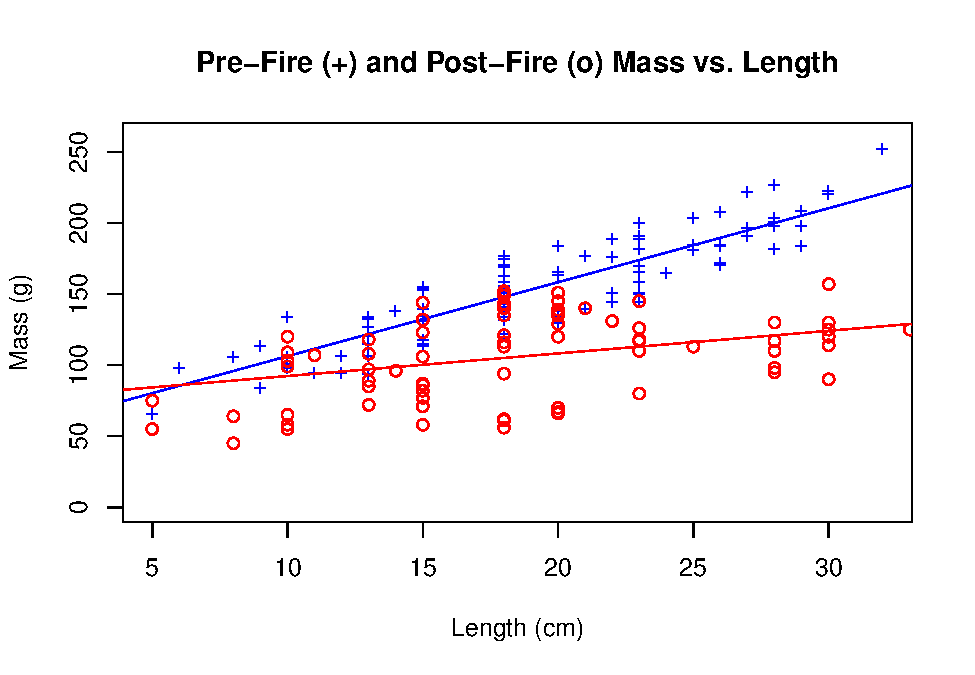
\includegraphics{Rportfolio-bookdown_files/figure-latex/unnamed-chunk-12-1.pdf}
\caption{\label{fig:unnamed-chunk-12}Scatterplot and linear regression line of fish length in centimeters versus fish mass in grams in Cache La Poudre in 2012 before the High Park Fire (blue, +) and in 2013 after the High Park Fire (red, o).}
\end{figure}

\hypertarget{extracting-and-visualizing-meteorological-data}{%
\chapter{Extracting and Visualizing Meteorological Data}\label{extracting-and-visualizing-meteorological-data}}

\begin{quote}
``What do you call dangerous precipitation? A rain of terror.''
\end{quote}

For this assignment, we used custom functions to read in and look at average meteorological data scraped from a public data archive.

Data is from \href{https://snowstudies.org/archived-data/}{Snowstudies.org}. Assignment by Dr.~Matthew Ross and Dr.~Nathan Mueller of Colorado State University.

\hypertarget{extract-the-meteorological-data-urls.-here-we-want-you-to-use-the-rvest-package-to-get-the-urls-for-the-sasp-forcing-and-sbsp_forcing-meteorological-datasets.}{%
\section{\texorpdfstring{1. Extract the meteorological data URLs. Here we want you to use the \texttt{rvest} package to get the URLs for the \texttt{SASP\ forcing} and \texttt{SBSP\_forcing} meteorological datasets.}{1. Extract the meteorological data URLs. Here we want you to use the rvest package to get the URLs for the SASP forcing and SBSP\_forcing meteorological datasets.}}\label{extract-the-meteorological-data-urls.-here-we-want-you-to-use-the-rvest-package-to-get-the-urls-for-the-sasp-forcing-and-sbsp_forcing-meteorological-datasets.}}

\begin{Shaded}
\begin{Highlighting}[]
\CommentTok{\# Read HTML page }
\NormalTok{snowarchive }\OtherTok{\textless{}{-}} \FunctionTok{read\_html}\NormalTok{(}\StringTok{"https://snowstudies.org/archived{-}data/"}\NormalTok{)}

\CommentTok{\# Read link with specific pattern}
\NormalTok{links }\OtherTok{\textless{}{-}}\NormalTok{ snowarchive }\SpecialCharTok{\%\textgreater{}\%}
  \FunctionTok{html\_nodes}\NormalTok{(}\StringTok{\textquotesingle{}a\textquotesingle{}}\NormalTok{) }\SpecialCharTok{\%\textgreater{}\%} \CommentTok{\#look for links}
\NormalTok{  .[}\FunctionTok{grepl}\NormalTok{(}\StringTok{\textquotesingle{}forcing\textquotesingle{}}\NormalTok{,.)] }\SpecialCharTok{\%\textgreater{}\%} \CommentTok{\#filter to only links with "forcing" term}
  \FunctionTok{html\_attr}\NormalTok{(}\StringTok{\textquotesingle{}href\textquotesingle{}}\NormalTok{) }\CommentTok{\#tell it these are urls}

\NormalTok{links }\CommentTok{\# view}
\end{Highlighting}
\end{Shaded}

\begin{verbatim}
## [1] "https://snowstudies.org/wp-content/uploads/2022/02/SBB_SASP_Forcing_Data.txt"
## [2] "https://snowstudies.org/wp-content/uploads/2022/02/SBB_SBSP_Forcing_Data.txt"
\end{verbatim}

\hypertarget{download-the-meteorological-data.-use-the-download_file-and-str_split_fixed-commands-to-download-the-data-and-save-it-in-your-data-folder.-you-can-use-a-for-loop-or-a-map-function.}{%
\section{\texorpdfstring{2. Download the meteorological data. Use the \texttt{download\_file} and \texttt{str\_split\_fixed} commands to download the data and save it in your data folder. You can use a for loop or a map function.}{2. Download the meteorological data. Use the download\_file and str\_split\_fixed commands to download the data and save it in your data folder. You can use a for loop or a map function.}}\label{download-the-meteorological-data.-use-the-download_file-and-str_split_fixed-commands-to-download-the-data-and-save-it-in-your-data-folder.-you-can-use-a-for-loop-or-a-map-function.}}

\begin{Shaded}
\begin{Highlighting}[]
\CommentTok{\# Grab only the name of the file by splitting out on forward slashes}
\NormalTok{splits }\OtherTok{\textless{}{-}} \FunctionTok{str\_split\_fixed}\NormalTok{(links,}\StringTok{\textquotesingle{}/\textquotesingle{}}\NormalTok{,}\DecValTok{8}\NormalTok{)}

\CommentTok{\#Keep only the 8th column}
\NormalTok{files }\OtherTok{\textless{}{-}}\NormalTok{ splits[,}\DecValTok{8}\NormalTok{] }

\NormalTok{files}
\end{Highlighting}
\end{Shaded}

\begin{verbatim}
## [1] "SBB_SASP_Forcing_Data.txt" "SBB_SBSP_Forcing_Data.txt"
\end{verbatim}

\begin{Shaded}
\begin{Highlighting}[]
\CommentTok{\# Generate a file list for where the data goes}
\NormalTok{file\_names }\OtherTok{\textless{}{-}} \FunctionTok{paste0}\NormalTok{(}\StringTok{\textquotesingle{}Data\_sci\_bookdown/data/snow/\textquotesingle{}}\NormalTok{, files)}

\CommentTok{\# For loop that downloads each {-} i for every instance, length function tells how many instances}
\ControlFlowTok{for}\NormalTok{(i }\ControlFlowTok{in} \DecValTok{1}\SpecialCharTok{:}\FunctionTok{length}\NormalTok{(file\_names))\{}
  \FunctionTok{download.file}\NormalTok{(links[i],}\AttributeTok{destfile=}\NormalTok{file\_names[i])}
\NormalTok{\}}

\CommentTok{\# Download via map function}
\CommentTok{\#map2(links, file\_names, download.file)}

\CommentTok{\# Map version of the for loop (downloading files)}
\NormalTok{downloaded }\OtherTok{\textless{}{-}} \FunctionTok{file.exists}\NormalTok{(file\_names) }
\NormalTok{evaluate }\OtherTok{\textless{}{-}} \SpecialCharTok{!}\FunctionTok{all}\NormalTok{(downloaded) }\CommentTok{\# sees if files are downloaded (T/F)}
\ControlFlowTok{if}\NormalTok{(evaluate }\SpecialCharTok{==}\NormalTok{ T)\{}
  \FunctionTok{map2}\NormalTok{(links[}\DecValTok{1}\SpecialCharTok{:}\DecValTok{2}\NormalTok{],file\_names[}\DecValTok{1}\SpecialCharTok{:}\DecValTok{2}\NormalTok{],download.file)}
\NormalTok{\}}\ControlFlowTok{else}\NormalTok{\{}\FunctionTok{print}\NormalTok{(}\StringTok{\textquotesingle{}data downloaded\textquotesingle{}}\NormalTok{)\}}
\end{Highlighting}
\end{Shaded}

\begin{verbatim}
## [1] "data downloaded"
\end{verbatim}

\hypertarget{write-a-custom-function-to-read-in-the-data-and-append-a-site-column-to-the-data.}{%
\section{3. Write a custom function to read in the data and append a site column to the data.}\label{write-a-custom-function-to-read-in-the-data-and-append-a-site-column-to-the-data.}}

\begin{Shaded}
\begin{Highlighting}[]
\CommentTok{\# Traditional read in}

\NormalTok{SASP }\OtherTok{\textless{}{-}} \FunctionTok{read.csv}\NormalTok{(}\StringTok{"Data\_sci\_bookdown/data/snow/SBB\_SASP\_Forcing\_Data.csv"}\NormalTok{) }\SpecialCharTok{\%\textgreater{}\%}
  \FunctionTok{select}\NormalTok{(}\DecValTok{1}\NormalTok{,}\DecValTok{2}\NormalTok{,}\DecValTok{3}\NormalTok{,}\DecValTok{7}\NormalTok{,}\DecValTok{10}\NormalTok{)}
  
\FunctionTok{colnames}\NormalTok{(SASP) }\OtherTok{\textless{}{-}} \FunctionTok{c}\NormalTok{(}\StringTok{"year"}\NormalTok{,}\StringTok{"month"}\NormalTok{,}\StringTok{"day"}\NormalTok{,}\StringTok{"precip"}\NormalTok{,}\StringTok{"temp"}\NormalTok{)}

\NormalTok{SBSP }\OtherTok{\textless{}{-}} \FunctionTok{read.csv}\NormalTok{(}\StringTok{"Data\_sci\_bookdown/data/snow/SBB\_SBSP\_Forcing\_Data.csv"}\NormalTok{) }\SpecialCharTok{\%\textgreater{}\%}
  \FunctionTok{select}\NormalTok{(}\DecValTok{1}\NormalTok{,}\DecValTok{2}\NormalTok{,}\DecValTok{3}\NormalTok{,}\DecValTok{7}\NormalTok{,}\DecValTok{10}\NormalTok{)}
  
\FunctionTok{colnames}\NormalTok{(SBSP) }\OtherTok{\textless{}{-}} \FunctionTok{c}\NormalTok{(}\StringTok{"year"}\NormalTok{,}\StringTok{"month"}\NormalTok{,}\StringTok{"day"}\NormalTok{,}\StringTok{"precip"}\NormalTok{,}\StringTok{"temp"}\NormalTok{)}

\CommentTok{\# Combine csvs}
\NormalTok{alldata }\OtherTok{\textless{}{-}} \FunctionTok{rbind}\NormalTok{(SASP,SBSP)}

\CommentTok{\# Read in via new function}

\CommentTok{\# Grab headers from metadata pdf}
\FunctionTok{library}\NormalTok{(pdftools)}
\end{Highlighting}
\end{Shaded}

\begin{verbatim}
## Using poppler version 20.12.1
\end{verbatim}

\begin{Shaded}
\begin{Highlighting}[]
\NormalTok{headers }\OtherTok{\textless{}{-}} \FunctionTok{pdf\_text}\NormalTok{(}\StringTok{\textquotesingle{}https://snowstudies.org/wp{-}content/uploads/2022/02/Serially{-}Complete{-}Metadata{-}text08.pdf\textquotesingle{}}\NormalTok{) }\SpecialCharTok{\%\textgreater{}\%}
\NormalTok{  readr}\SpecialCharTok{::}\FunctionTok{read\_lines}\NormalTok{(.) }\SpecialCharTok{\%\textgreater{}\%}
  \FunctionTok{trimws}\NormalTok{(.) }\SpecialCharTok{\%\textgreater{}\%}
  \FunctionTok{str\_split\_fixed}\NormalTok{(.,}\StringTok{\textquotesingle{}}\SpecialCharTok{\textbackslash{}\textbackslash{}}\StringTok{.\textquotesingle{}}\NormalTok{,}\DecValTok{2}\NormalTok{) }\SpecialCharTok{\%\textgreater{}\%}
\NormalTok{  .[,}\DecValTok{2}\NormalTok{] }\SpecialCharTok{\%\textgreater{}\%}
\NormalTok{  .[}\DecValTok{1}\SpecialCharTok{:}\DecValTok{26}\NormalTok{] }\SpecialCharTok{\%\textgreater{}\%}
  \FunctionTok{str\_trim}\NormalTok{(}\AttributeTok{side =} \StringTok{"left"}\NormalTok{)}
\end{Highlighting}
\end{Shaded}

\hypertarget{use-the-map-function-to-read-in-both-meteorological-files.-display-a-summary-of-your-tibble.}{%
\section{\texorpdfstring{4. Use the \texttt{map} function to read in both meteorological files. Display a summary of your tibble.}{4. Use the map function to read in both meteorological files. Display a summary of your tibble.}}\label{use-the-map-function-to-read-in-both-meteorological-files.-display-a-summary-of-your-tibble.}}

\begin{Shaded}
\begin{Highlighting}[]
\CommentTok{\# Pull site name out of the file name and read in the .txt files}
\NormalTok{read\_data }\OtherTok{\textless{}{-}} \ControlFlowTok{function}\NormalTok{(file)\{}
\NormalTok{  name }\OtherTok{=} \FunctionTok{str\_split\_fixed}\NormalTok{(file,}\StringTok{\textquotesingle{}\_\textquotesingle{}}\NormalTok{,}\DecValTok{2}\NormalTok{)[,}\DecValTok{2}\NormalTok{] }\SpecialCharTok{\%\textgreater{}\%} 
    \FunctionTok{gsub}\NormalTok{(}\StringTok{\textquotesingle{}\_Forcing\_Data.txt\textquotesingle{}}\NormalTok{,}\StringTok{\textquotesingle{}\textquotesingle{}}\NormalTok{,.) }
\NormalTok{  df }\OtherTok{\textless{}{-}} \FunctionTok{read\_fwf}\NormalTok{(file) }\SpecialCharTok{\%\textgreater{}\%} 
    \FunctionTok{select}\NormalTok{(}\AttributeTok{year=}\DecValTok{1}\NormalTok{, }\AttributeTok{month=}\DecValTok{2}\NormalTok{, }\AttributeTok{day=}\DecValTok{3}\NormalTok{, }\AttributeTok{hour=}\DecValTok{4}\NormalTok{, }\AttributeTok{precip=}\DecValTok{7}\NormalTok{, }\AttributeTok{air\_temp=}\DecValTok{10}\NormalTok{) }\SpecialCharTok{\%\textgreater{}\%} \CommentTok{\#choose and name columns}
    \FunctionTok{mutate}\NormalTok{(}\AttributeTok{site =}\NormalTok{ name) }\CommentTok{\#add column }
\NormalTok{\}}

\NormalTok{alldata2 }\OtherTok{\textless{}{-}} \FunctionTok{map\_dfr}\NormalTok{(file\_names,read\_data) }
\end{Highlighting}
\end{Shaded}

\begin{verbatim}
## Rows: 69168 Columns: 19
## -- Column specification --------------------------------------------------------
## 
## chr  (2): X12, X14
## dbl (17): X1, X2, X3, X4, X5, X6, X7, X8, X9, X10, X11, X13, X15, X16, X17, ...
## 
## i Use `spec()` to retrieve the full column specification for this data.
## i Specify the column types or set `show_col_types = FALSE` to quiet this message.
## Rows: 69168 Columns: 19
## -- Column specification --------------------------------------------------------
## 
## chr  (2): X12, X14
## dbl (17): X1, X2, X3, X4, X5, X6, X7, X8, X9, X10, X11, X13, X15, X16, X17, ...
## 
## i Use `spec()` to retrieve the full column specification for this data.
## i Specify the column types or set `show_col_types = FALSE` to quiet this message.
\end{verbatim}

\begin{Shaded}
\begin{Highlighting}[]
\FunctionTok{summary}\NormalTok{(alldata2)}
\end{Highlighting}
\end{Shaded}

\begin{verbatim}
##       year          month             day             hour      
##  Min.   :2003   Min.   : 1.000   Min.   : 1.00   Min.   : 0.00  
##  1st Qu.:2005   1st Qu.: 3.000   1st Qu.: 8.00   1st Qu.: 5.75  
##  Median :2007   Median : 6.000   Median :16.00   Median :11.50  
##  Mean   :2007   Mean   : 6.472   Mean   :15.76   Mean   :11.50  
##  3rd Qu.:2009   3rd Qu.: 9.000   3rd Qu.:23.00   3rd Qu.:17.25  
##  Max.   :2011   Max.   :12.000   Max.   :31.00   Max.   :23.00  
##      precip             air_temp         site          
##  Min.   :0.000e+00   Min.   :242.1   Length:138336     
##  1st Qu.:0.000e+00   1st Qu.:265.8   Class :character  
##  Median :0.000e+00   Median :272.6   Mode  :character  
##  Mean   :3.838e-05   Mean   :272.6                     
##  3rd Qu.:0.000e+00   3rd Qu.:279.7                     
##  Max.   :6.111e-03   Max.   :295.8
\end{verbatim}

\hypertarget{make-a-line-plot-of-mean-temp-by-year-by-site-using-the-air-temp-k-variable.-is-there-anything-suspicious-in-the-plot-adjust-your-filtering-if-needed.}{%
\section{\texorpdfstring{5. Make a line plot of mean temp by year by site (using the \texttt{air\ temp\ {[}K{]}} variable). Is there anything suspicious in the plot? Adjust your filtering if needed.}{5. Make a line plot of mean temp by year by site (using the air temp {[}K{]} variable). Is there anything suspicious in the plot? Adjust your filtering if needed.}}\label{make-a-line-plot-of-mean-temp-by-year-by-site-using-the-air-temp-k-variable.-is-there-anything-suspicious-in-the-plot-adjust-your-filtering-if-needed.}}

\begin{Shaded}
\begin{Highlighting}[]
\NormalTok{temp\_yearly }\OtherTok{\textless{}{-}}\NormalTok{ alldata2 }\SpecialCharTok{\%\textgreater{}\%} 
\FunctionTok{group\_by}\NormalTok{(year, site) }\SpecialCharTok{\%\textgreater{}\%}
\FunctionTok{summarise}\NormalTok{(}\AttributeTok{mean\_temp =} \FunctionTok{mean}\NormalTok{(}\StringTok{\textasciigrave{}}\AttributeTok{air\_temp}\StringTok{\textasciigrave{}}\NormalTok{, }\AttributeTok{na.rm=}\NormalTok{T))}
\end{Highlighting}
\end{Shaded}

\begin{verbatim}
## `summarise()` has grouped output by 'year'. You can override using the `.groups`
## argument.
\end{verbatim}

\begin{Shaded}
\begin{Highlighting}[]
\FunctionTok{ggplot}\NormalTok{(temp\_yearly,}\FunctionTok{aes}\NormalTok{(}\AttributeTok{x=}\NormalTok{year, }\AttributeTok{y=}\NormalTok{mean\_temp, }\AttributeTok{color=}\NormalTok{site)) }\SpecialCharTok{+} 
  \FunctionTok{geom\_point}\NormalTok{() }\SpecialCharTok{+} \FunctionTok{geom\_line}\NormalTok{() }\SpecialCharTok{+}
  \FunctionTok{xlab}\NormalTok{(}\StringTok{"Year"}\NormalTok{) }\SpecialCharTok{+} \FunctionTok{ylab}\NormalTok{(}\StringTok{"Mean Temperature (Degrees Kelvin)"}\NormalTok{) }\SpecialCharTok{+}
\NormalTok{  ggthemes}\SpecialCharTok{::}\FunctionTok{theme\_few}\NormalTok{() }\SpecialCharTok{+} 
  \FunctionTok{scale\_color\_brewer}\NormalTok{(}\AttributeTok{palette =} \StringTok{"Set2"}\NormalTok{) }\SpecialCharTok{+} 
  \FunctionTok{scale\_x\_continuous}\NormalTok{(}\AttributeTok{breaks =} \FunctionTok{pretty}\NormalTok{(}\FunctionTok{c}\NormalTok{(}\DecValTok{2003}\NormalTok{,}\DecValTok{2012}\NormalTok{), }\AttributeTok{n =} \DecValTok{6}\NormalTok{)) }\SpecialCharTok{+}
  \FunctionTok{theme}\NormalTok{(}\AttributeTok{legend.position=}\StringTok{"bottom"}\NormalTok{)}
\end{Highlighting}
\end{Shaded}

\begin{figure}
\centering
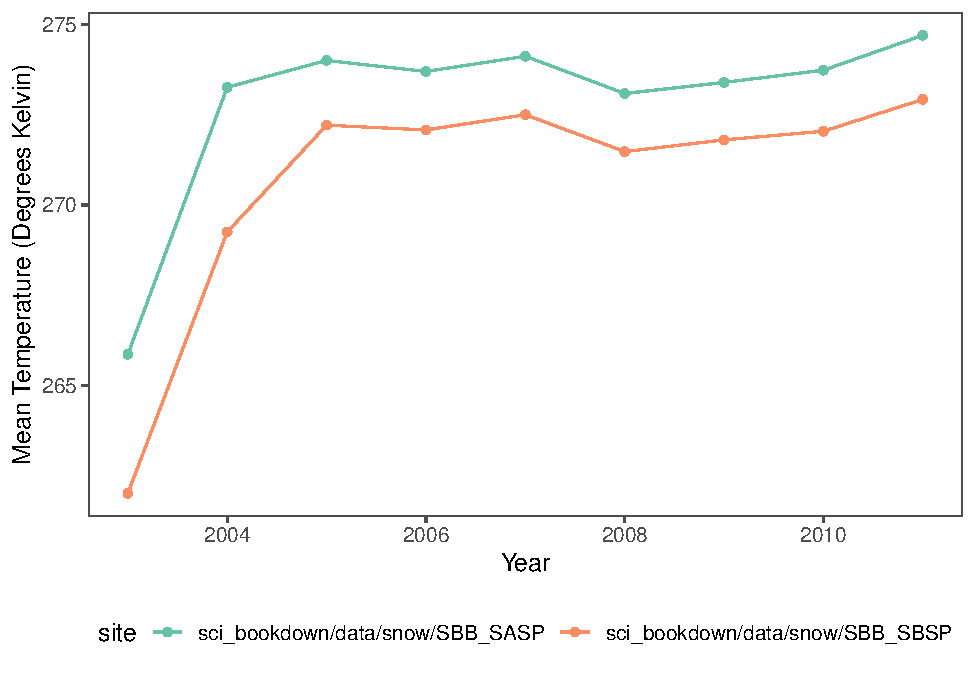
\includegraphics{Rportfolio-bookdown_files/figure-latex/unnamed-chunk-17-1.pdf}
\caption{\label{fig:unnamed-chunk-17}Mean temperature of the SASP (teal) and SBSP (orange) sites from 2003 to 2012, in degrees Kelvin.}
\end{figure}

\hypertarget{write-a-function-that-makes-line-plots-of-monthly-average-temperature-at-each-site-for-a-given-year.-use-a-for-loop-to-make-these-plots-for-2005-to-2010.}{%
\section{6. Write a function that makes line plots of monthly average temperature at each site for a given year. Use a for loop to make these plots for 2005 to 2010.}\label{write-a-function-that-makes-line-plots-of-monthly-average-temperature-at-each-site-for-a-given-year.-use-a-for-loop-to-make-these-plots-for-2005-to-2010.}}

\begin{Shaded}
\begin{Highlighting}[]
\NormalTok{temp\_monthly }\OtherTok{\textless{}{-}}\NormalTok{ alldata2 }\SpecialCharTok{\%\textgreater{}\%}
    \FunctionTok{group\_by}\NormalTok{(year, month, site) }\SpecialCharTok{\%\textgreater{}\%}
    \FunctionTok{summarize}\NormalTok{(}\AttributeTok{mean\_temp =} \FunctionTok{mean}\NormalTok{(}\StringTok{\textasciigrave{}}\AttributeTok{air\_temp}\StringTok{\textasciigrave{}}\NormalTok{, }\AttributeTok{na.rm=}\NormalTok{T))}
\end{Highlighting}
\end{Shaded}

\begin{verbatim}
## `summarise()` has grouped output by 'year', 'month'. You can override using the
## `.groups` argument.
\end{verbatim}

\begin{Shaded}
\begin{Highlighting}[]
\FunctionTok{par}\NormalTok{(}\AttributeTok{mfrow=}\FunctionTok{c}\NormalTok{(}\DecValTok{5}\NormalTok{,}\DecValTok{1}\NormalTok{))}

\NormalTok{plot\_monthly }\OtherTok{\textless{}{-}} \ControlFlowTok{function}\NormalTok{(year.no) \{}
\NormalTok{  plot }\OtherTok{\textless{}{-}}\NormalTok{ temp\_monthly }\SpecialCharTok{\%\textgreater{}\%}
    \FunctionTok{filter}\NormalTok{(year }\SpecialCharTok{==}\NormalTok{ year.no) }\SpecialCharTok{\%\textgreater{}\%}
    \FunctionTok{ggplot}\NormalTok{(}\FunctionTok{aes}\NormalTok{(}\AttributeTok{x=}\NormalTok{month, }\AttributeTok{y=}\NormalTok{mean\_temp, }\AttributeTok{color=}\NormalTok{site)) }\SpecialCharTok{+} 
      \FunctionTok{geom\_line}\NormalTok{() }\SpecialCharTok{+}
      \FunctionTok{xlab}\NormalTok{(}\StringTok{"Month"}\NormalTok{) }\SpecialCharTok{+} \FunctionTok{ylab}\NormalTok{(}\StringTok{"Mean Temperature (Degrees Kelvin)"}\NormalTok{) }\SpecialCharTok{+}
\NormalTok{      ggthemes}\SpecialCharTok{::}\FunctionTok{theme\_few}\NormalTok{() }\SpecialCharTok{+} 
      \FunctionTok{scale\_color\_brewer}\NormalTok{(}\AttributeTok{palette =} \StringTok{"Set2"}\NormalTok{) }\SpecialCharTok{+} 
      \FunctionTok{scale\_x\_discrete}\NormalTok{(}\AttributeTok{limits =} \FunctionTok{c}\NormalTok{(}\DecValTok{1}\NormalTok{,}\DecValTok{2}\NormalTok{,}\DecValTok{3}\NormalTok{,}\DecValTok{4}\NormalTok{,}\DecValTok{5}\NormalTok{,}\DecValTok{6}\NormalTok{,}\DecValTok{7}\NormalTok{,}\DecValTok{8}\NormalTok{,}\DecValTok{9}\NormalTok{,}\DecValTok{10}\NormalTok{,}\DecValTok{11}\NormalTok{,}\DecValTok{12}\NormalTok{)) }\SpecialCharTok{+}
      \FunctionTok{scale\_y\_continuous}\NormalTok{(}\AttributeTok{breaks =} \FunctionTok{pretty}\NormalTok{(}\FunctionTok{c}\NormalTok{(}\DecValTok{255}\NormalTok{,}\DecValTok{290}\NormalTok{), }\AttributeTok{n =} \DecValTok{4}\NormalTok{)) }\SpecialCharTok{+}
      \FunctionTok{theme}\NormalTok{(}\AttributeTok{legend.position=}\StringTok{"bottom"}\NormalTok{)}
  \FunctionTok{print}\NormalTok{(plot)}
\NormalTok{  \}}

\ControlFlowTok{for}\NormalTok{(i }\ControlFlowTok{in} \DecValTok{2005}\SpecialCharTok{:}\DecValTok{2010}\NormalTok{)\{}
  \FunctionTok{plot\_monthly}\NormalTok{(i)}
\NormalTok{\}}
\end{Highlighting}
\end{Shaded}

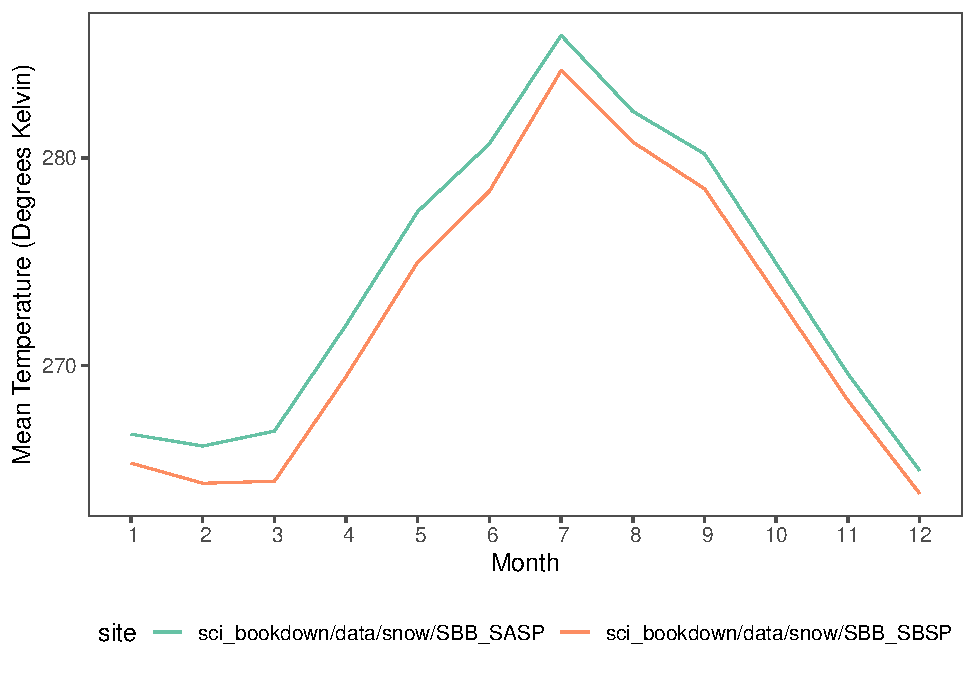
\includegraphics{Rportfolio-bookdown_files/figure-latex/unnamed-chunk-18-1.pdf} 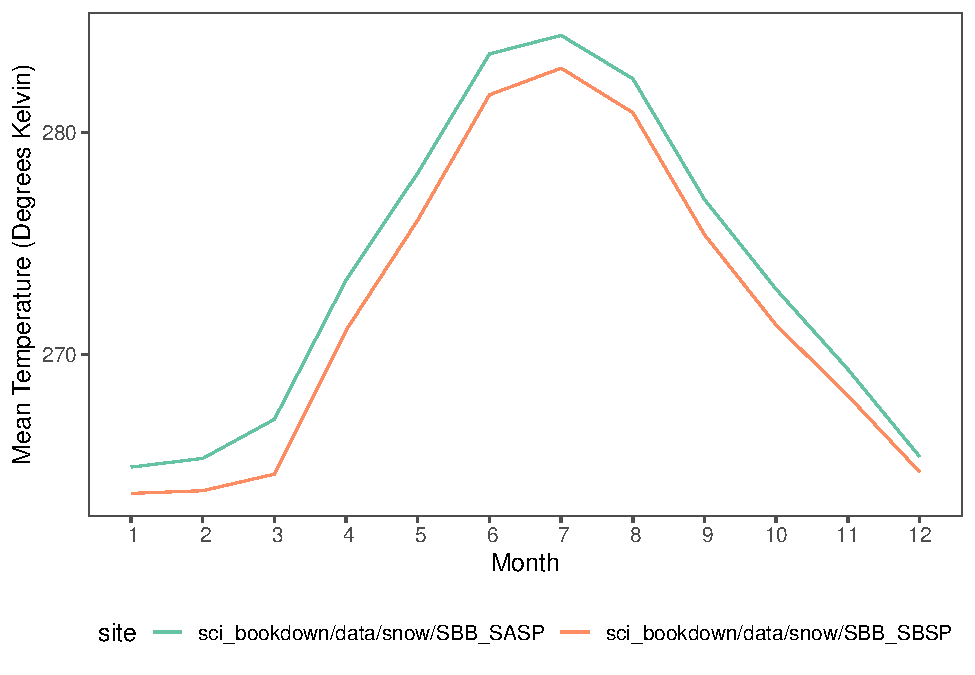
\includegraphics{Rportfolio-bookdown_files/figure-latex/unnamed-chunk-18-2.pdf} 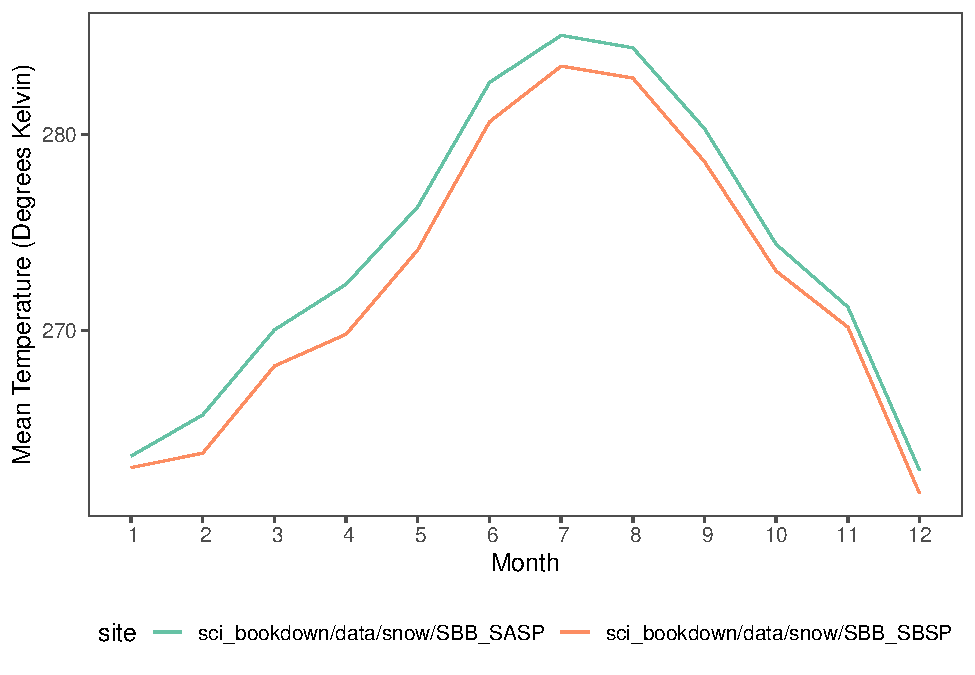
\includegraphics{Rportfolio-bookdown_files/figure-latex/unnamed-chunk-18-3.pdf} 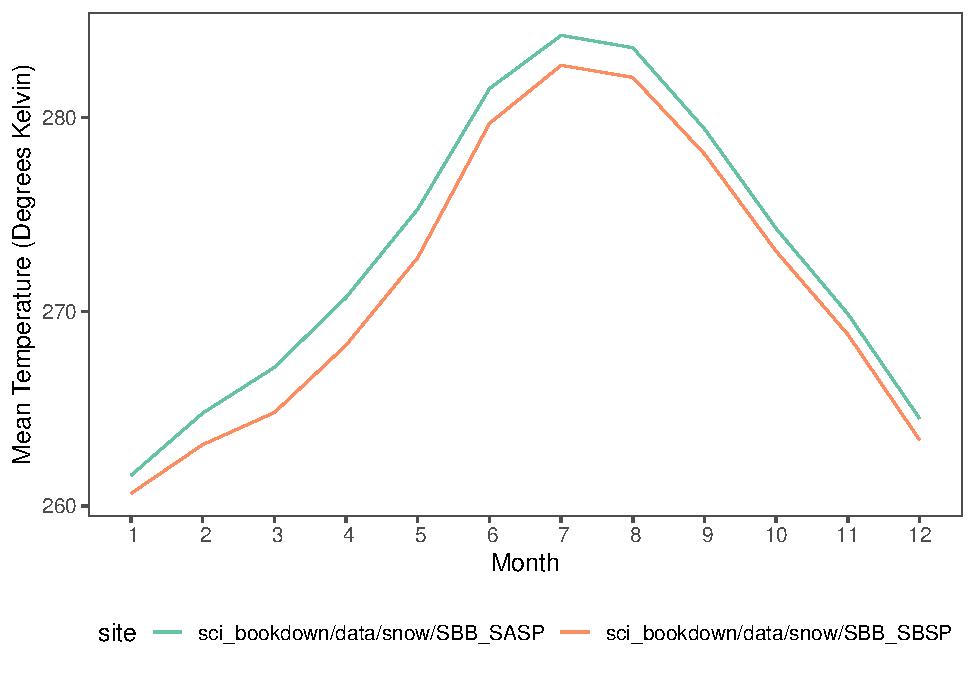
\includegraphics{Rportfolio-bookdown_files/figure-latex/unnamed-chunk-18-4.pdf} 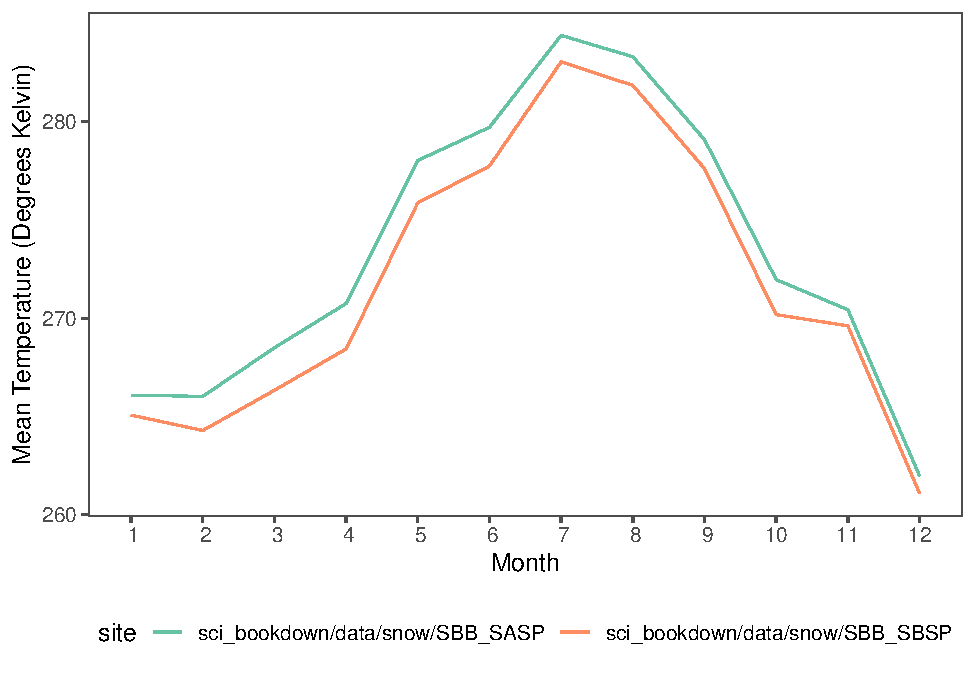
\includegraphics{Rportfolio-bookdown_files/figure-latex/unnamed-chunk-18-5.pdf} 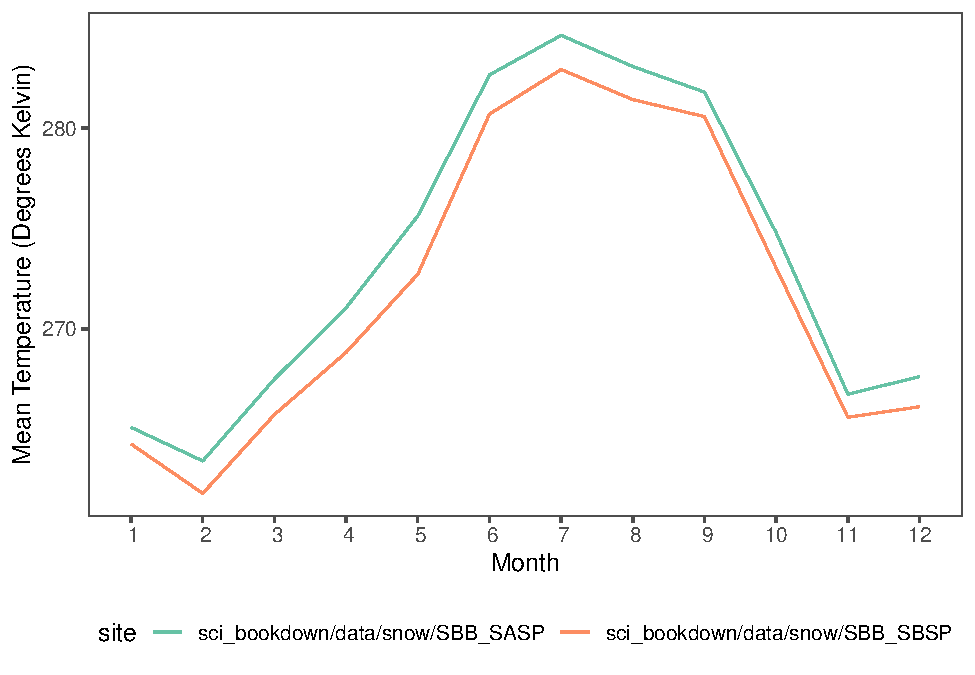
\includegraphics{Rportfolio-bookdown_files/figure-latex/unnamed-chunk-18-6.pdf}

\hypertarget{bonus-make-a-plot-of-average-daily-precipitation-by-day-of-year-averaged-across-all-available-years}{%
\section{Bonus: Make a plot of average daily precipitation by day of year (averaged across all available years)}\label{bonus-make-a-plot-of-average-daily-precipitation-by-day-of-year-averaged-across-all-available-years}}

\begin{Shaded}
\begin{Highlighting}[]
\NormalTok{precip\_daily }\OtherTok{\textless{}{-}}\NormalTok{ alldata2 }\SpecialCharTok{\%\textgreater{}\%}
  \FunctionTok{mutate}\NormalTok{(}\AttributeTok{date =} \FunctionTok{make\_date}\NormalTok{(year, month, day),}
                \AttributeTok{day\_no =} \FunctionTok{yday}\NormalTok{(date)) }\SpecialCharTok{\%\textgreater{}\%}
  \FunctionTok{group\_by}\NormalTok{(day\_no) }\SpecialCharTok{\%\textgreater{}\%}
  \FunctionTok{summarize}\NormalTok{(}\AttributeTok{mean\_precip =} \FunctionTok{mean}\NormalTok{(}\StringTok{\textasciigrave{}}\AttributeTok{precip}\StringTok{\textasciigrave{}}\SpecialCharTok{*}\DecValTok{86400}\NormalTok{, }\AttributeTok{na.rm=}\NormalTok{T))}

\FunctionTok{ggplot}\NormalTok{(precip\_daily, }\FunctionTok{aes}\NormalTok{(}\AttributeTok{x=}\NormalTok{day\_no, }\AttributeTok{y=}\NormalTok{mean\_precip)) }\SpecialCharTok{+} 
      \FunctionTok{geom\_line}\NormalTok{() }\SpecialCharTok{+}
      \FunctionTok{xlab}\NormalTok{(}\StringTok{"Day of Year"}\NormalTok{) }\SpecialCharTok{+} \FunctionTok{ylab}\NormalTok{(}\StringTok{"Mean Precipitation (mm/day)"}\NormalTok{) }\SpecialCharTok{+}
\NormalTok{      ggthemes}\SpecialCharTok{::}\FunctionTok{theme\_few}\NormalTok{() }\SpecialCharTok{+} 
      \FunctionTok{scale\_color\_brewer}\NormalTok{(}\AttributeTok{palette =} \StringTok{"Set2"}\NormalTok{) }\SpecialCharTok{+} 
      \FunctionTok{scale\_y\_continuous}\NormalTok{(}\AttributeTok{breaks =} \FunctionTok{pretty}\NormalTok{(}\FunctionTok{c}\NormalTok{(}\DecValTok{0}\NormalTok{,}\DecValTok{14}\NormalTok{), }\AttributeTok{n =} \DecValTok{7}\NormalTok{)) }\SpecialCharTok{+}
      \FunctionTok{scale\_x\_continuous}\NormalTok{(}\AttributeTok{breaks =} \FunctionTok{pretty}\NormalTok{(}\FunctionTok{c}\NormalTok{(}\DecValTok{1}\NormalTok{,}\DecValTok{365}\NormalTok{), }\AttributeTok{n =} \DecValTok{8}\NormalTok{))}
\end{Highlighting}
\end{Shaded}

\begin{figure}
\centering
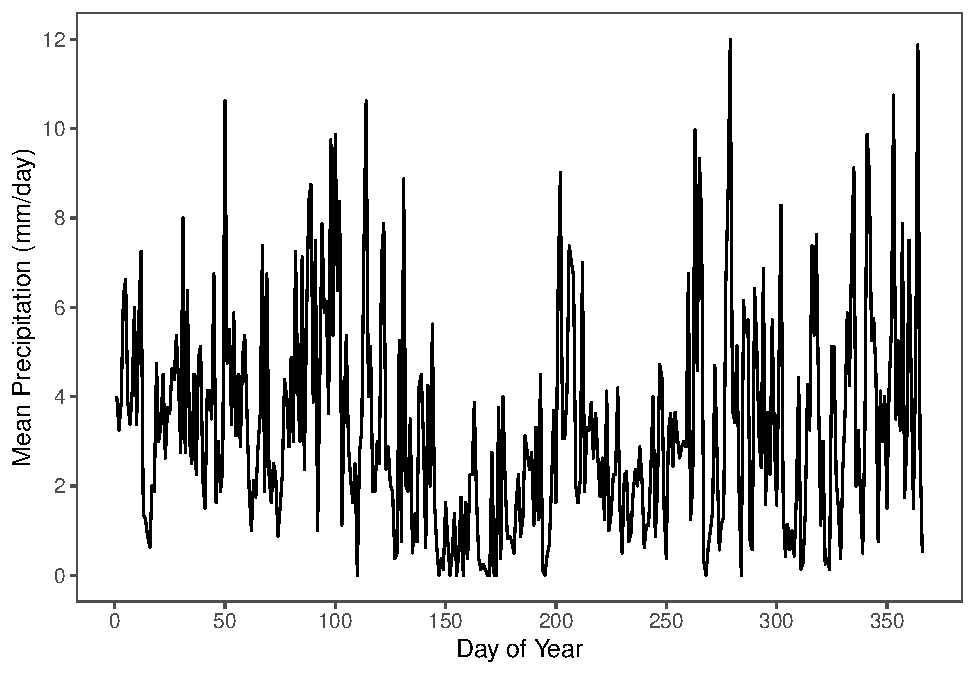
\includegraphics{Rportfolio-bookdown_files/figure-latex/unnamed-chunk-19-1.pdf}
\caption{\label{fig:unnamed-chunk-19}Mean daily precipitation by day of year, averaged from 2003 to 2012.}
\end{figure}

\hypertarget{spatial-analysis-in-r}{%
\chapter{Spatial Analysis in R}\label{spatial-analysis-in-r}}

\begin{quote}
``Why are latitude and longitude so smart? Because they have so many degrees!''
\end{quote}

In this assignment, I learned to use R for spatial analyses.

Data is from the \href{https://lagoslakes.org/}{LAGOS dataset}. Assignment by Dr.~Matthew Ross and Dr.~Nathan Mueller of Colorado State University.

\hypertarget{loading-in-data}{%
\section{Loading in data}\label{loading-in-data}}

\hypertarget{first-download-and-then-specifically-grab-the-locus-or-site-lat-longs}{%
\subsection{First download and then specifically grab the locus (or site lat longs)}\label{first-download-and-then-specifically-grab-the-locus-or-site-lat-longs}}

\begin{Shaded}
\begin{Highlighting}[]
\CommentTok{\# \#Lagos download script}
\CommentTok{\#LAGOSNE::lagosne\_get(dest\_folder = LAGOSNE:::lagos\_path(), overwrite = TRUE)}


\CommentTok{\#Load in lagos}
\NormalTok{lagos }\OtherTok{\textless{}{-}} \FunctionTok{lagosne\_load}\NormalTok{()}
\end{Highlighting}
\end{Shaded}

\begin{verbatim}
## Warning in (function (version = NULL, fpath = NA) : LAGOSNE version unspecified,
## loading version: 1.087.3
\end{verbatim}

\begin{Shaded}
\begin{Highlighting}[]
\CommentTok{\#Grab the lake centroid info}
\NormalTok{lake\_centers }\OtherTok{\textless{}{-}}\NormalTok{ lagos}\SpecialCharTok{$}\NormalTok{locus}

\CommentTok{\# Make an sf object }
\NormalTok{spatial\_lakes }\OtherTok{\textless{}{-}} \FunctionTok{st\_as\_sf}\NormalTok{(lake\_centers,}\AttributeTok{coords=}\FunctionTok{c}\NormalTok{(}\StringTok{\textquotesingle{}nhd\_long\textquotesingle{}}\NormalTok{,}\StringTok{\textquotesingle{}nhd\_lat\textquotesingle{}}\NormalTok{),}
                          \AttributeTok{crs=}\DecValTok{4326}\NormalTok{)}

\CommentTok{\#Grab the water quality data}
\NormalTok{nutr }\OtherTok{\textless{}{-}}\NormalTok{ lagos}\SpecialCharTok{$}\NormalTok{epi\_nutr}

\CommentTok{\#Look at column names}
\CommentTok{\#names(nutr)}
\end{Highlighting}
\end{Shaded}

\hypertarget{convert-to-spatial-data}{%
\subsection{Convert to spatial data}\label{convert-to-spatial-data}}

\begin{Shaded}
\begin{Highlighting}[]
\CommentTok{\#Look at the column names}
\CommentTok{\#names(lake\_centers)}

\CommentTok{\#Look at the structure}
\CommentTok{\#str(lake\_centers)}

\CommentTok{\#View the full dataset}
\CommentTok{\#View(lake\_centers \%\textgreater{}\% slice(1:100))}

\NormalTok{spatial\_lakes }\OtherTok{\textless{}{-}} \FunctionTok{st\_as\_sf}\NormalTok{(}\AttributeTok{x =}\NormalTok{ lake\_centers, }\AttributeTok{coords =} \FunctionTok{c}\NormalTok{(}\StringTok{"nhd\_long"}\NormalTok{,}\StringTok{"nhd\_lat"}\NormalTok{), }\AttributeTok{crs =} \DecValTok{4326}\NormalTok{) }\SpecialCharTok{\%\textgreater{}\%}
  \FunctionTok{st\_transform}\NormalTok{(}\DecValTok{2163}\NormalTok{)}

\CommentTok{\#mapview(spatial\_lakes)}

\CommentTok{\#Subset for plotting}
\NormalTok{subset\_spatial }\OtherTok{\textless{}{-}}\NormalTok{ spatial\_lakes }\SpecialCharTok{\%\textgreater{}\%}
  \FunctionTok{slice}\NormalTok{(}\DecValTok{1}\SpecialCharTok{:}\DecValTok{100}\NormalTok{) }

\NormalTok{subset\_baser }\OtherTok{\textless{}{-}}\NormalTok{ spatial\_lakes[}\DecValTok{1}\SpecialCharTok{:}\DecValTok{100}\NormalTok{,]}

\CommentTok{\#Dynamic mapviewer}
\CommentTok{\#mapview(subset\_spatial)}
\end{Highlighting}
\end{Shaded}

\hypertarget{subset-to-only-minnesota}{%
\subsection{Subset to only Minnesota}\label{subset-to-only-minnesota}}

\begin{Shaded}
\begin{Highlighting}[]
\NormalTok{states }\OtherTok{\textless{}{-}} \FunctionTok{us\_states}\NormalTok{()}

\CommentTok{\#Plot all the states to check if they loaded}
\CommentTok{\#mapview(states)}

\NormalTok{minnesota }\OtherTok{\textless{}{-}}\NormalTok{ states }\SpecialCharTok{\%\textgreater{}\%}
  \FunctionTok{filter}\NormalTok{(name }\SpecialCharTok{==} \StringTok{\textquotesingle{}Minnesota\textquotesingle{}}\NormalTok{) }\SpecialCharTok{\%\textgreater{}\%}
  \FunctionTok{st\_transform}\NormalTok{(}\DecValTok{2163}\NormalTok{)}
\CommentTok{\#mapview(minnesota)}

\CommentTok{\#Subset lakes based on spatial position}
\NormalTok{minnesota\_lakes }\OtherTok{\textless{}{-}}\NormalTok{ spatial\_lakes[minnesota,]}

\CommentTok{\#Plotting the first 1000 lakes}
\NormalTok{minnesota\_lakes }\SpecialCharTok{\%\textgreater{}\%}
  \FunctionTok{arrange}\NormalTok{(}\SpecialCharTok{{-}}\NormalTok{lake\_area\_ha) }\SpecialCharTok{\%\textgreater{}\%}
    \FunctionTok{slice}\NormalTok{(}\DecValTok{1}\SpecialCharTok{:}\DecValTok{1000}\NormalTok{)}
\end{Highlighting}
\end{Shaded}

\begin{verbatim}
## Simple feature collection with 1000 features and 16 fields
## Geometry type: POINT
## Dimension:     XY
## Bounding box:  xmin: 254441 ymin: -154522.4 xmax: 755222.3 ymax: 464949.4
## Projected CRS: NAD27 / US National Atlas Equal Area
## First 10 features:
##    lagoslakeid     nhdid           gnis_name lake_area_ha lake_perim_meters
## 1        15162 123319728   Lake of the Woods   123779.817         401005.02
## 2        34986 105567868      Lower Red Lake    66650.332         115825.47
## 3         2498 120019294     Mille Lacs Lake    51867.225         151701.94
## 4        39213 105567402      Upper Red Lake    48288.325          99828.05
## 5          996 120018981          Leech Lake    41824.352         344259.98
## 6          583 120019513 Lake Winnibigoshish    22566.124          86722.10
## 7           73 120019354          Rainy Lake    18522.551         660313.32
## 8         2554 105954753      Vermilion Lake    15736.590         509617.01
## 9         2161 120019371     Kabetogama Lake     9037.249         288750.31
## 10        3119 166868528           Cass Lake     8375.173          85326.14
##    nhd_fcode nhd_ftype iws_zoneid hu4_zoneid hu6_zoneid hu8_zoneid hu12_zoneid
## 1      39004       390  IWS_37547     HU4_26     HU6_36    HU8_468  HU12_13912
## 2      39004       390  IWS_34899     HU4_54     HU6_74    HU8_327  HU12_14600
## 3      39004       390  IWS_22933     HU4_25     HU6_73    HU8_344  HU12_10875
## 4      39004       390  IWS_33471     HU4_54     HU6_74    HU8_327  HU12_14204
## 5      39004       390  IWS_23572     HU4_25     HU6_35    HU8_332  HU12_14479
## 6      39004       390  IWS_22455     HU4_25     HU6_35    HU8_331  HU12_14543
## 7      39004       390  IWS_37542     HU4_26     HU6_36    HU8_473  HU12_13942
## 8      39004       390  IWS_36424     HU4_26     HU6_36    HU8_131  HU12_14405
## 9      39004       390  IWS_36301     HU4_26     HU6_36    HU8_130  HU12_14395
## 10     39004       390  IWS_21080     HU4_25     HU6_35    HU8_331  HU12_13957
##    edu_zoneid county_zoneid state_zoneid elevation_m                  geometry
## 1      EDU_56    County_435     State_14    323.5090 POINT (366706.2 464949.4)
## 2      EDU_16    County_455     State_14    358.1656 POINT (371974.2 341706.5)
## 3      EDU_43    County_484     State_14    381.7920 POINT (489582.1 157109.5)
## 4      EDU_16    County_455     State_14    358.3096 POINT (389013.3 360819.5)
## 5      EDU_42    County_424     State_14    395.2420 POINT (422409.7 255724.9)
## 6      EDU_42    County_424     State_14    396.1560   POINT (437872.1 286675)
## 7      EDU_55    County_446     State_14    338.0670 POINT (515833.6 420274.2)
## 8       EDU_3    County_446     State_14    414.1680 POINT (566966.7 347059.1)
## 9      EDU_55    County_446     State_14    339.2530 POINT (519199.2 408290.2)
## 10     EDU_42    County_424     State_14    396.7710 POINT (410563.2 281005.2)
\end{verbatim}

\begin{Shaded}
\begin{Highlighting}[]
  \CommentTok{\#mapview(.,zcol = \textquotesingle{}lake\_area\_ha\textquotesingle{})}
\end{Highlighting}
\end{Shaded}

\hypertarget{part-one}{%
\section{Part one}\label{part-one}}

\hypertarget{show-a-map-outline-of-iowa-and-illinois-similar-to-minnesota-map-upstream}{%
\subsection{Show a map outline of Iowa and Illinois (similar to Minnesota map upstream)}\label{show-a-map-outline-of-iowa-and-illinois-similar-to-minnesota-map-upstream}}

\begin{Shaded}
\begin{Highlighting}[]
\NormalTok{Istates }\OtherTok{\textless{}{-}}\NormalTok{ states }\SpecialCharTok{\%\textgreater{}\%}
  \FunctionTok{filter}\NormalTok{(name }\SpecialCharTok{==} \StringTok{\textquotesingle{}Iowa\textquotesingle{}}\SpecialCharTok{|}\NormalTok{ name}\SpecialCharTok{==} \StringTok{\textquotesingle{}Illinois\textquotesingle{}}\NormalTok{) }\SpecialCharTok{\%\textgreater{}\%}
  \FunctionTok{st\_transform}\NormalTok{(}\DecValTok{2163}\NormalTok{)}
\FunctionTok{mapview}\NormalTok{(Istates, }\AttributeTok{canvas =} \ConstantTok{TRUE}\NormalTok{) }
\end{Highlighting}
\end{Shaded}

\hypertarget{subset-lagos-data-to-these-sites-how-many-sites-are-in-illinois-and-iowa-combined-how-does-this-compare-to-minnesota}{%
\subsection{Subset LAGOS data to these sites, how many sites are in Illinois and Iowa combined? How does this compare to Minnesota?}\label{subset-lagos-data-to-these-sites-how-many-sites-are-in-illinois-and-iowa-combined-how-does-this-compare-to-minnesota}}

\begin{Shaded}
\begin{Highlighting}[]
\NormalTok{Istates\_lakes }\OtherTok{\textless{}{-}}\NormalTok{ spatial\_lakes[Istates,]}

\FunctionTok{nrow}\NormalTok{(Istates\_lakes)}
\end{Highlighting}
\end{Shaded}

\begin{verbatim}
## [1] 16466
\end{verbatim}

\begin{Shaded}
\begin{Highlighting}[]
\NormalTok{Istates\_count }\OtherTok{\textless{}{-}} \FunctionTok{length}\NormalTok{(Istates\_lakes}\SpecialCharTok{$}\NormalTok{lagoslakeid)}

\FunctionTok{nrow}\NormalTok{(minnesota\_lakes)}
\end{Highlighting}
\end{Shaded}

\begin{verbatim}
## [1] 29038
\end{verbatim}

\begin{Shaded}
\begin{Highlighting}[]
\NormalTok{Minn\_count }\OtherTok{\textless{}{-}} \FunctionTok{length}\NormalTok{(minnesota\_lakes}\SpecialCharTok{$}\NormalTok{lagoslakeid)}
\end{Highlighting}
\end{Shaded}

Iowa and Illinois have 16466 lakes combined, much less than the number of lakes that Minnesota alone has, 29038.

\hypertarget{what-is-the-distribution-of-lake-size-in-iowa-vs.-minnesota}{%
\subsection{What is the distribution of lake size in Iowa vs.~Minnesota?}\label{what-is-the-distribution-of-lake-size-in-iowa-vs.-minnesota}}

\begin{itemize}
\tightlist
\item
  Here I want to see a histogram plot with lake size on x-axis and frequency on y axis (check out geom\_histogram)
\end{itemize}

\begin{Shaded}
\begin{Highlighting}[]
\NormalTok{iowa }\OtherTok{\textless{}{-}}\NormalTok{ states }\SpecialCharTok{\%\textgreater{}\%}
  \FunctionTok{filter}\NormalTok{(name }\SpecialCharTok{==} \StringTok{\textquotesingle{}Iowa\textquotesingle{}}\NormalTok{) }\SpecialCharTok{\%\textgreater{}\%}
  \FunctionTok{st\_transform}\NormalTok{(}\DecValTok{2163}\NormalTok{)}

\NormalTok{iowa\_lakes }\OtherTok{\textless{}{-}}\NormalTok{ spatial\_lakes[iowa,]}

\NormalTok{combined }\OtherTok{\textless{}{-}} \FunctionTok{rbind}\NormalTok{(iowa\_lakes, minnesota\_lakes)}

\FunctionTok{ggplot}\NormalTok{(combined, }\FunctionTok{aes}\NormalTok{(}\AttributeTok{x=}\NormalTok{ lake\_area\_ha)) }\SpecialCharTok{+} 
\NormalTok{  ggthemes}\SpecialCharTok{::}\FunctionTok{theme\_few}\NormalTok{() }\SpecialCharTok{+} \FunctionTok{theme}\NormalTok{(}\AttributeTok{legend.position=}\StringTok{"bottom"}\NormalTok{) }\SpecialCharTok{+}
  \FunctionTok{xlab}\NormalTok{(}\StringTok{"Lake Area (ha)"}\NormalTok{) }\SpecialCharTok{+} \FunctionTok{ylab}\NormalTok{(}\StringTok{"Count"}\NormalTok{) }\SpecialCharTok{+}
  \FunctionTok{scale\_x\_continuous}\NormalTok{(}\AttributeTok{trans =} \StringTok{"log10"}\NormalTok{, }\AttributeTok{labels =}\NormalTok{ scales}\SpecialCharTok{::}\NormalTok{comma) }\SpecialCharTok{+}
  \FunctionTok{geom\_histogram}\NormalTok{(}\AttributeTok{data =}\NormalTok{ minnesota\_lakes, }\AttributeTok{color =} \StringTok{"red"}\NormalTok{, }\AttributeTok{alpha =} \FloatTok{0.2}\NormalTok{) }\SpecialCharTok{+} 
  \FunctionTok{geom\_histogram}\NormalTok{(}\AttributeTok{data =}\NormalTok{ iowa\_lakes, }\AttributeTok{color =} \StringTok{"blue"}\NormalTok{, }\AttributeTok{alpha =} \FloatTok{0.2}\NormalTok{) }\SpecialCharTok{+}
  \FunctionTok{scale\_fill\_manual}\NormalTok{(}\AttributeTok{values=}\FunctionTok{c}\NormalTok{(}\StringTok{"blue"}\NormalTok{,}\StringTok{"red"}\NormalTok{), }\StringTok{"State"}\NormalTok{)}
\end{Highlighting}
\end{Shaded}

\begin{verbatim}
## `stat_bin()` using `bins = 30`. Pick better value with `binwidth`.
## `stat_bin()` using `bins = 30`. Pick better value with `binwidth`.
\end{verbatim}

\begin{figure}
\centering
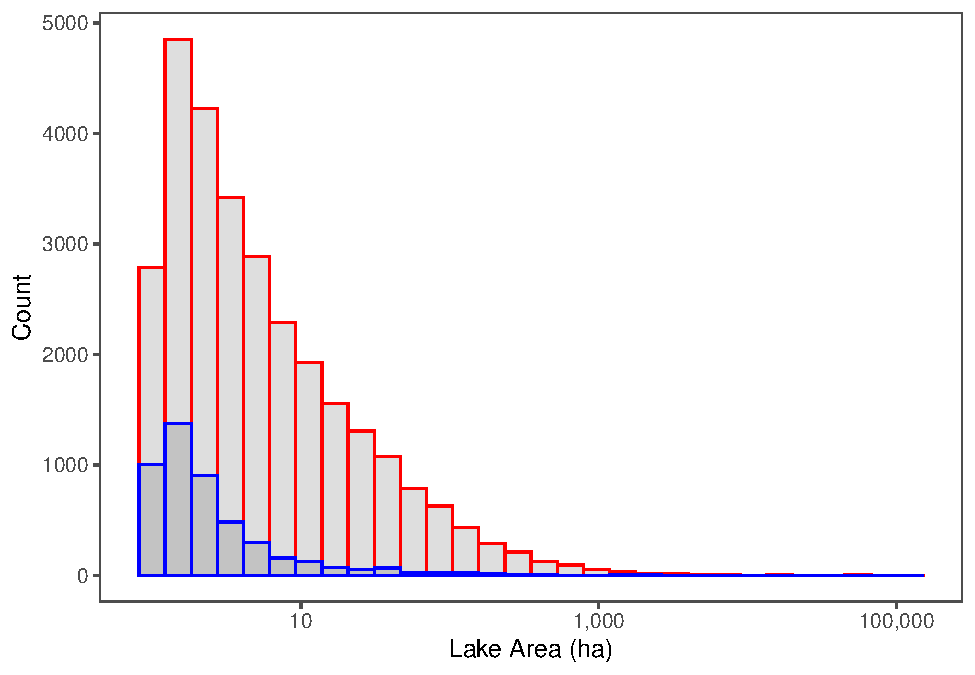
\includegraphics{Rportfolio-bookdown_files/figure-latex/unnamed-chunk-24-1.pdf}
\caption{\label{fig:unnamed-chunk-24}The number of lakes with a given area, in hectares, in Minnesota (red) and Iowa (blue).}
\end{figure}

\hypertarget{make-an-interactive-plot-of-lakes-in-iowa-and-illinois-and-color-them-by-lake-area-in-hectares}{%
\subsection{Make an interactive plot of lakes in Iowa and Illinois and color them by lake area in hectares}\label{make-an-interactive-plot-of-lakes-in-iowa-and-illinois-and-color-them-by-lake-area-in-hectares}}

\begin{Shaded}
\begin{Highlighting}[]
\NormalTok{Istates\_map }\OtherTok{=}\NormalTok{ Istates\_lakes }\SpecialCharTok{\%\textgreater{}\%}
  \FunctionTok{arrange}\NormalTok{(}\SpecialCharTok{{-}}\NormalTok{lake\_area\_ha) }\SpecialCharTok{\%\textgreater{}\%}
    \FunctionTok{slice}\NormalTok{(}\DecValTok{1}\SpecialCharTok{:}\DecValTok{1000}\NormalTok{)}

\FunctionTok{mapview}\NormalTok{(Istates\_map, }\AttributeTok{zcol =} \StringTok{\textquotesingle{}lake\_area\_ha\textquotesingle{}}\NormalTok{,  }\AttributeTok{canvas =} \ConstantTok{TRUE}\NormalTok{) }
\end{Highlighting}
\end{Shaded}

\hypertarget{what-other-data-sources-might-we-use-to-understand-how-reservoirs-and-natural-lakes-vary-in-size-in-these-three-states}{%
\subsection{What other data sources might we use to understand how reservoirs and natural lakes vary in size in these three states?}\label{what-other-data-sources-might-we-use-to-understand-how-reservoirs-and-natural-lakes-vary-in-size-in-these-three-states}}

We might use the US Geological Survey (USGS) National Water Informational System (NWIS) and its National Water Dashboard as a data source, and look at gage height (indicating lake depth) as another parameter for lake size variation. The USGS National Hydrography Dataset (NHD) is another data source that would, similarly to Lagos, give us a surface area metric for lakes in the various states.

\hypertarget{part-two}{%
\section{Part two}\label{part-two}}

\hypertarget{subsets}{%
\subsection{Subsets}\label{subsets}}

\hypertarget{columns-nutr-to-only-keep-key-info-that-we-want}{%
\subsubsection{Columns nutr to only keep key info that we want}\label{columns-nutr-to-only-keep-key-info-that-we-want}}

\begin{Shaded}
\begin{Highlighting}[]
\NormalTok{clarity\_only }\OtherTok{\textless{}{-}}\NormalTok{ nutr }\SpecialCharTok{\%\textgreater{}\%}
\NormalTok{  dplyr}\SpecialCharTok{::}\FunctionTok{select}\NormalTok{(lagoslakeid,sampledate,chla,doc,secchi) }\SpecialCharTok{\%\textgreater{}\%}
  \FunctionTok{mutate}\NormalTok{(}\AttributeTok{sampledate =} \FunctionTok{as.character}\NormalTok{(sampledate) }\SpecialCharTok{\%\textgreater{}\%} \FunctionTok{ymd}\NormalTok{(.))}
\end{Highlighting}
\end{Shaded}

\hypertarget{keep-sites-with-at-least-200-observations}{%
\subsubsection{Keep sites with at least 200 observations}\label{keep-sites-with-at-least-200-observations}}

\begin{Shaded}
\begin{Highlighting}[]
\CommentTok{\#Look at the number of rows of dataset}
\CommentTok{\#nrow(clarity\_only)}

\NormalTok{chla\_secchi }\OtherTok{\textless{}{-}}\NormalTok{ clarity\_only }\SpecialCharTok{\%\textgreater{}\%}
  \FunctionTok{filter}\NormalTok{(}\SpecialCharTok{!}\FunctionTok{is.na}\NormalTok{(chla),}
         \SpecialCharTok{!}\FunctionTok{is.na}\NormalTok{(secchi))}

\CommentTok{\# How many observatiosn did we lose?}
\CommentTok{\# nrow(clarity\_only) {-} nrow(chla\_secchi)}


\CommentTok{\# Keep only the lakes with at least 200 observations of secchi and chla}
\NormalTok{chla\_secchi\_200 }\OtherTok{\textless{}{-}}\NormalTok{ chla\_secchi }\SpecialCharTok{\%\textgreater{}\%}
  \FunctionTok{group\_by}\NormalTok{(lagoslakeid) }\SpecialCharTok{\%\textgreater{}\%}
  \FunctionTok{mutate}\NormalTok{(}\AttributeTok{count =} \FunctionTok{n}\NormalTok{()) }\SpecialCharTok{\%\textgreater{}\%}
  \FunctionTok{filter}\NormalTok{(count }\SpecialCharTok{\textgreater{}} \DecValTok{200}\NormalTok{)}
\end{Highlighting}
\end{Shaded}

\hypertarget{join-water-quality-data-to-spatial-data}{%
\subsubsection{Join water quality data to spatial data}\label{join-water-quality-data-to-spatial-data}}

\begin{Shaded}
\begin{Highlighting}[]
\NormalTok{spatial\_200 }\OtherTok{\textless{}{-}} \FunctionTok{inner\_join}\NormalTok{(spatial\_lakes,chla\_secchi\_200 }\SpecialCharTok{\%\textgreater{}\%}
                            \FunctionTok{distinct}\NormalTok{(lagoslakeid,}\AttributeTok{.keep\_all=}\NormalTok{T),}
                          \AttributeTok{by=}\StringTok{\textquotesingle{}lagoslakeid\textquotesingle{}}\NormalTok{)}
\end{Highlighting}
\end{Shaded}

\hypertarget{mean-chlorophyll-a-map}{%
\subsection{Mean Chlorophyll A map}\label{mean-chlorophyll-a-map}}

\begin{Shaded}
\begin{Highlighting}[]
\DocumentationTok{\#\#\# Take the mean chl\_a and secchi by lake}

\NormalTok{means\_200 }\OtherTok{\textless{}{-}}\NormalTok{ chla\_secchi\_200 }\SpecialCharTok{\%\textgreater{}\%}
  \CommentTok{\# Take summary by lake id}
  \FunctionTok{group\_by}\NormalTok{(lagoslakeid) }\SpecialCharTok{\%\textgreater{}\%}
  \CommentTok{\# take mean chl\_a per lake id}
  \FunctionTok{summarize}\NormalTok{(}\AttributeTok{mean\_chl =} \FunctionTok{mean}\NormalTok{(chla,}\AttributeTok{na.rm=}\NormalTok{T),}
            \AttributeTok{mean\_secchi=}\FunctionTok{mean}\NormalTok{(secchi,}\AttributeTok{na.rm=}\NormalTok{T)) }\SpecialCharTok{\%\textgreater{}\%}
  \CommentTok{\#Get rid of NAs}
  \FunctionTok{filter}\NormalTok{(}\SpecialCharTok{!}\FunctionTok{is.na}\NormalTok{(mean\_chl),}
         \SpecialCharTok{!}\FunctionTok{is.na}\NormalTok{(mean\_secchi)) }\SpecialCharTok{\%\textgreater{}\%}
  \CommentTok{\# Take the log base 10 of the mean\_chl}
  \FunctionTok{mutate}\NormalTok{(}\AttributeTok{log10\_mean\_chl =} \FunctionTok{log10}\NormalTok{(mean\_chl))}

\CommentTok{\#Join datasets}
\NormalTok{mean\_spatial }\OtherTok{\textless{}{-}} \FunctionTok{inner\_join}\NormalTok{(spatial\_lakes,means\_200,}
                          \AttributeTok{by=}\StringTok{\textquotesingle{}lagoslakeid\textquotesingle{}}\NormalTok{) }

\CommentTok{\#Make a map}
\FunctionTok{mapview}\NormalTok{(mean\_spatial, }\AttributeTok{zcol=}\StringTok{\textquotesingle{}log10\_mean\_chl\textquotesingle{}}\NormalTok{, }\AttributeTok{layer.name =} \StringTok{"Mean Chlorophyll A Content"}\NormalTok{)}
\end{Highlighting}
\end{Shaded}

\hypertarget{what-is-the-correlation-between-secchi-disk-depth-and-chlorophyll-a-for-sites-with-at-least-200-observations}{%
\subsection{What is the correlation between Secchi Disk Depth and Chlorophyll a for sites with at least 200 observations?}\label{what-is-the-correlation-between-secchi-disk-depth-and-chlorophyll-a-for-sites-with-at-least-200-observations}}

\begin{Shaded}
\begin{Highlighting}[]
\FunctionTok{ggplot}\NormalTok{(means\_200) }\SpecialCharTok{+}
  \FunctionTok{geom\_point}\NormalTok{(}\FunctionTok{aes}\NormalTok{(mean\_secchi, mean\_chl)) }\SpecialCharTok{+}
\NormalTok{  ggthemes}\SpecialCharTok{::}\FunctionTok{theme\_few}\NormalTok{() }\SpecialCharTok{+} 
  \FunctionTok{xlab}\NormalTok{(}\StringTok{"Mean Secchi Disk Depth"}\NormalTok{) }\SpecialCharTok{+} \FunctionTok{ylab}\NormalTok{(}\StringTok{"Mean Chlorophyll Content"}\NormalTok{)}
\end{Highlighting}
\end{Shaded}

\begin{figure}
\centering
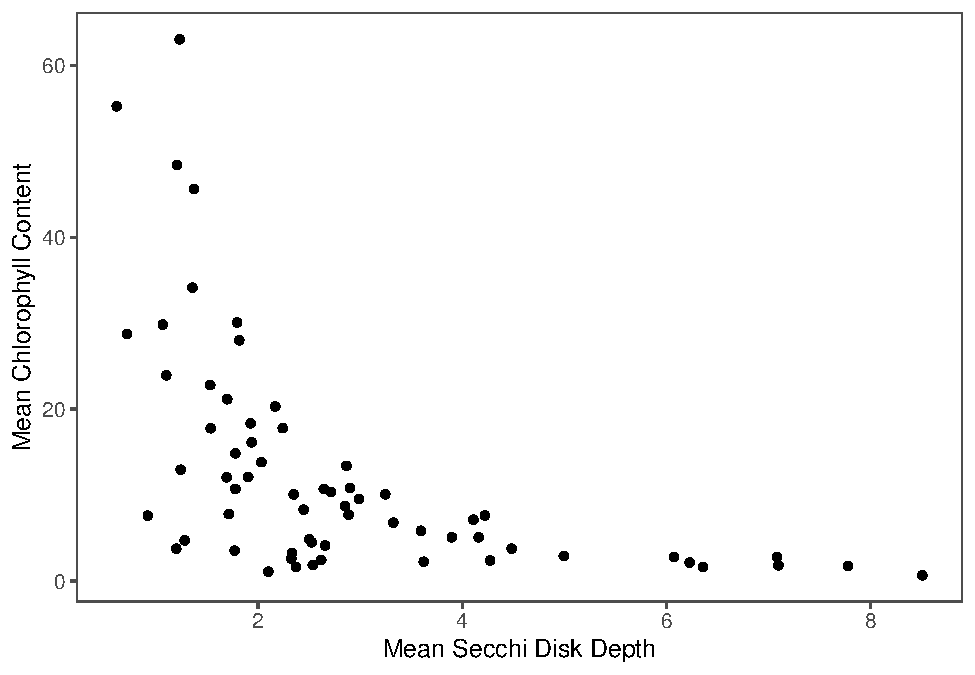
\includegraphics{Rportfolio-bookdown_files/figure-latex/unnamed-chunk-30-1.pdf}
\caption{\label{fig:unnamed-chunk-30}Chlorophyll content has a negative correlation with Secchi disk depth at sites with at least 200 observations.}
\end{figure}

\hypertarget{why-might-this-be-the-case}{%
\subsubsection{Why might this be the case?}\label{why-might-this-be-the-case}}

Secchi disks measure water clarity; the deeper the disk, the clearer the water (1). Chlorophyll content in lakes is generally a reliable marker of algae content, so that high chlorophyll values indicate high algal biomass and corresponding low water clarity (2). Additionally, chlorophyll may be used as a proxy for water quality, since high algal biomass is associated with high nutrient pollution in the process of eutrophication (2). High pollution may further decrease water clarity, so that the relationship between chlorophyll and Secchi disk depth may be expected.

\begin{enumerate}
\def\labelenumi{\arabic{enumi}.}
\item
  ``The Secchi Dip-in - What Is a Secchi Disk?'' North American Lake Management Society (NALMS),
  \url{https://www.nalms.org/secchidipin/monitoring-methods/the-secchi-disk/what-is-a-secchi-disk/}.
\item
  Filazzola, A., Mahdiyan, O., Shuvo, A. et al.~A database of chlorophyll and water chemistry in freshwater lakes. Sci Data 7, 310 (2020).
  \url{https://doi-org.ezproxy2.library.colostate.edu/10.1038/s41597-020-00648-2}
\end{enumerate}

\hypertarget{what-states-have-the-most-data}{%
\subsection{What states have the most data?}\label{what-states-have-the-most-data}}

\hypertarget{make-a-lagos-spatial-dataset-that-has-the-total-number-of-counts-per-site.}{%
\subsubsection{Make a lagos spatial dataset that has the total number of counts per site.}\label{make-a-lagos-spatial-dataset-that-has-the-total-number-of-counts-per-site.}}

\begin{Shaded}
\begin{Highlighting}[]
\NormalTok{site\_counts }\OtherTok{\textless{}{-}}\NormalTok{ chla\_secchi }\SpecialCharTok{\%\textgreater{}\%}
  \FunctionTok{group\_by}\NormalTok{(lagoslakeid) }\SpecialCharTok{\%\textgreater{}\%}
  \FunctionTok{mutate}\NormalTok{(}\AttributeTok{count =} \FunctionTok{n}\NormalTok{())}

\NormalTok{lake\_counts }\OtherTok{\textless{}{-}} \FunctionTok{inner\_join}\NormalTok{(site\_counts, lake\_centers, }\AttributeTok{by=} \StringTok{"lagoslakeid"}\NormalTok{)}\SpecialCharTok{\%\textgreater{}\%} 
\NormalTok{  dplyr}\SpecialCharTok{::}\FunctionTok{select}\NormalTok{(lagoslakeid,nhd\_long,nhd\_lat, count, secchi, chla)}

\NormalTok{spatial\_counts }\OtherTok{\textless{}{-}} \FunctionTok{st\_as\_sf}\NormalTok{(lake\_counts,}\AttributeTok{coords=}\FunctionTok{c}\NormalTok{(}\StringTok{"nhd\_long"}\NormalTok{,}\StringTok{"nhd\_lat"}\NormalTok{),}
                          \AttributeTok{crs=}\DecValTok{4326}\NormalTok{)}
\end{Highlighting}
\end{Shaded}

\hypertarget{join-this-point-dataset-to-the-us_boundaries-data.}{%
\subsubsection{Join this point dataset to the us\_boundaries data.}\label{join-this-point-dataset-to-the-us_boundaries-data.}}

\begin{Shaded}
\begin{Highlighting}[]
\NormalTok{states }\OtherTok{\textless{}{-}} \FunctionTok{us\_states}\NormalTok{()}

\NormalTok{states\_counts }\OtherTok{\textless{}{-}} \FunctionTok{st\_join}\NormalTok{(spatial\_counts, states)}
\end{Highlighting}
\end{Shaded}

\hypertarget{group-by-state-and-sum-all-the-observations-in-that-state-and-arrange-that-data-from-most-to-least-total-observations-per-state.}{%
\subsubsection{Group by state and sum all the observations in that state and arrange that data from most to least total observations per state.}\label{group-by-state-and-sum-all-the-observations-in-that-state-and-arrange-that-data-from-most-to-least-total-observations-per-state.}}

\begin{Shaded}
\begin{Highlighting}[]
\NormalTok{sum\_statecount }\OtherTok{\textless{}{-}}\NormalTok{ states\_counts }\SpecialCharTok{\%\textgreater{}\%}
  \FunctionTok{group\_by}\NormalTok{(state\_name) }\SpecialCharTok{\%\textgreater{}\%}
  \FunctionTok{summarize}\NormalTok{(}\AttributeTok{sum =} \FunctionTok{sum}\NormalTok{(count)) }\SpecialCharTok{\%\textgreater{}\%}
  \FunctionTok{arrange}\NormalTok{(}\FunctionTok{desc}\NormalTok{(sum)) }

\NormalTok{sumtable }\OtherTok{\textless{}{-}} \FunctionTok{tibble}\NormalTok{(sum\_statecount)}

\FunctionTok{view}\NormalTok{(sumtable)}

\CommentTok{\#ggplot(data = sumtable, aes(x=state\_name, y=sum, fill=state\_name)) + }
\CommentTok{\#  geom\_bar(stat = "identity", width = 0.3, position = "dodge") + }
\CommentTok{\#  ggthemes::theme\_few() +}
\CommentTok{\#  xlab("State") + ylab(expression(paste("\# of Observations"))) }
\end{Highlighting}
\end{Shaded}

Minnesota has the most observations. Vermont, has the next most observations, but less than half of Minnesota's observations. South Dakota has the least number of observations in the dataset.

\hypertarget{is-there-a-spatial-pattern-in-secchi-disk-depth-for-lakes-with-at-least-200-observations}{%
\subsection{Is there a spatial pattern in Secchi disk depth for lakes with at least 200 observations?}\label{is-there-a-spatial-pattern-in-secchi-disk-depth-for-lakes-with-at-least-200-observations}}

\begin{Shaded}
\begin{Highlighting}[]
\FunctionTok{mapview}\NormalTok{(mean\_spatial, }\AttributeTok{zcol=}\StringTok{\textquotesingle{}mean\_secchi\textquotesingle{}}\NormalTok{, }\AttributeTok{layer.name =} \StringTok{"Mean Secchi Disk Depth"}\NormalTok{)}
\end{Highlighting}
\end{Shaded}

\hypertarget{linear-regressions-quadratic-fits-residuals-and-spatial}{%
\chapter{Linear Regressions, Quadratic Fits, Residuals, and Spatial}\label{linear-regressions-quadratic-fits-residuals-and-spatial}}

\begin{quote}
``How many data scientists does it take to change a light bulb? That depends. It is really a matter of power.''
\end{quote}

This assignment combined several methods to look at relationships between crop yields and weather data over time.

Data from \href{https://quickstats.nass.usda.gov/}{USDA National Agricultural Statistical Service (NASS)}. Assignment by Dr.~Matthew Ross and Dr.~Nathan Mueller of Colorado State University.

\hypertarget{weather-data-analysis}{%
\section{Weather Data Analysis}\label{weather-data-analysis}}

\hypertarget{load-the-prism-daily-maximum-temperatures}{%
\subsection{Load the PRISM daily maximum temperatures}\label{load-the-prism-daily-maximum-temperatures}}

\begin{Shaded}
\begin{Highlighting}[]
\CommentTok{\# daily max temperature}
\CommentTok{\# dimensions: counties x days x years}
\NormalTok{prism }\OtherTok{\textless{}{-}} \FunctionTok{readMat}\NormalTok{(}\StringTok{"Data\_sci\_bookdown/data/prismiowa.mat"}\NormalTok{)}

\CommentTok{\# look at county \#1}
\NormalTok{t\_1981\_c1 }\OtherTok{\textless{}{-}}\NormalTok{ prism}\SpecialCharTok{$}\NormalTok{tmaxdaily.iowa[}\DecValTok{1}\NormalTok{,,}\DecValTok{1}\NormalTok{] }\CommentTok{\#first county, all days, first year}
\NormalTok{t\_1981\_c1[}\DecValTok{366}\NormalTok{] }\CommentTok{\#check for leap year (366 days)}
\end{Highlighting}
\end{Shaded}

\begin{verbatim}
## [1] NaN
\end{verbatim}

\begin{Shaded}
\begin{Highlighting}[]
\FunctionTok{plot}\NormalTok{(}\DecValTok{1}\SpecialCharTok{:}\DecValTok{366}\NormalTok{, t\_1981\_c1, }\AttributeTok{type =} \StringTok{"l"}\NormalTok{) }\CommentTok{\#base r plot}
\end{Highlighting}
\end{Shaded}

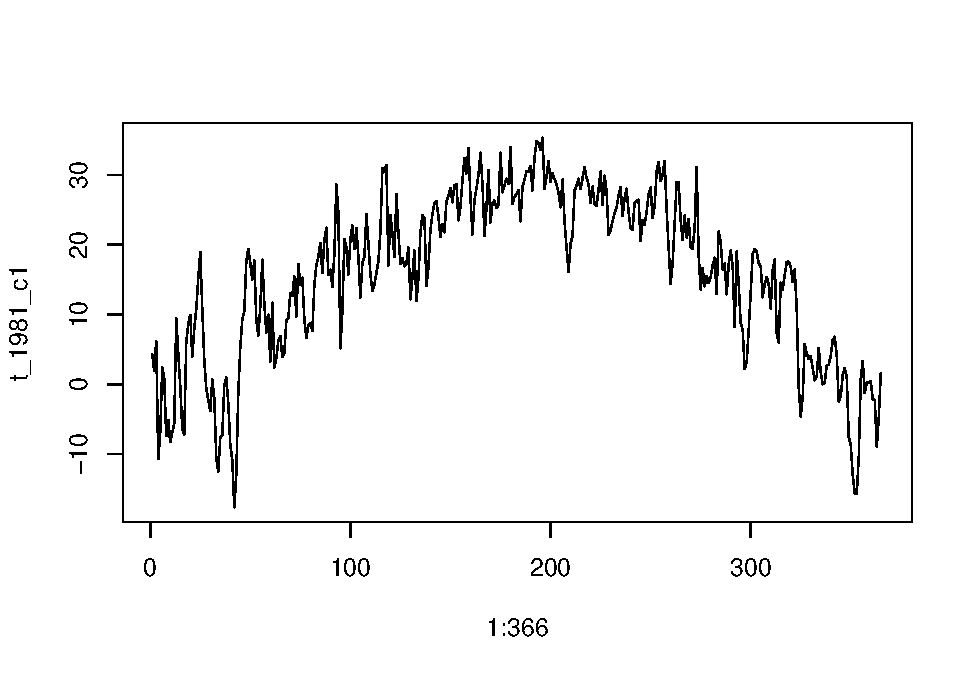
\includegraphics{Rportfolio-bookdown_files/figure-latex/tmax data-1.pdf}

\begin{Shaded}
\begin{Highlighting}[]
\CommentTok{\# assign dimension names to tmax matrix}
\FunctionTok{dimnames}\NormalTok{(prism}\SpecialCharTok{$}\NormalTok{tmaxdaily.iowa) }\OtherTok{\textless{}{-}} \FunctionTok{list}\NormalTok{(prism}\SpecialCharTok{$}\NormalTok{COUNTYFP, }\DecValTok{1}\SpecialCharTok{:}\DecValTok{366}\NormalTok{, prism}\SpecialCharTok{$}\NormalTok{years) }\CommentTok{\#add dimension names}

\CommentTok{\# converted 3d matrix into a data frame}
\NormalTok{tmaxdf }\OtherTok{\textless{}{-}} \FunctionTok{as.data.frame.table}\NormalTok{(prism}\SpecialCharTok{$}\NormalTok{tmaxdaily.iowa)}

\CommentTok{\# relabel the columns}
\FunctionTok{colnames}\NormalTok{(tmaxdf) }\OtherTok{\textless{}{-}} \FunctionTok{c}\NormalTok{(}\StringTok{"countyfp"}\NormalTok{,}\StringTok{"doy"}\NormalTok{,}\StringTok{"year"}\NormalTok{,}\StringTok{"tmax"}\NormalTok{) }\CommentTok{\#name columns}
\NormalTok{tmaxdf }\OtherTok{\textless{}{-}} \FunctionTok{tibble}\NormalTok{(tmaxdf) }\CommentTok{\#tidyverse table}
\end{Highlighting}
\end{Shaded}

\hypertarget{download-nass-corn-yield-data}{%
\subsection{Download NASS corn yield data}\label{download-nass-corn-yield-data}}

\begin{Shaded}
\begin{Highlighting}[]
\CommentTok{\# set our API key with NASS}
\FunctionTok{nassqs\_auth}\NormalTok{(}\AttributeTok{key =} \StringTok{"B9113AF8{-}85C4{-}3CEE{-}8D93{-}6E885D49E24F"}\NormalTok{) }\CommentTok{\#Here put in API code from USDA QuickStats service}

\CommentTok{\# parameters to query on }
\NormalTok{params }\OtherTok{\textless{}{-}} \FunctionTok{list}\NormalTok{(}\AttributeTok{commodity\_desc =} \StringTok{"CORN"}\NormalTok{, }\AttributeTok{util\_practice\_desc =} \StringTok{"GRAIN"}\NormalTok{, }\AttributeTok{prodn\_practice\_desc =} \StringTok{"ALL PRODUCTION PRACTICES"}\NormalTok{, }\AttributeTok{year\_\_GE =} \DecValTok{1981}\NormalTok{, }\AttributeTok{state\_alpha =} \StringTok{"IA"}\NormalTok{)}

\CommentTok{\# download}
\NormalTok{cornyieldsall }\OtherTok{\textless{}{-}} \FunctionTok{nassqs\_yields}\NormalTok{(params)}
\end{Highlighting}
\end{Shaded}

\begin{verbatim}
##   |                                                                              |                                                                      |   0%  |                                                                              |                                                                      |   1%  |                                                                              |=                                                                     |   1%  |                                                                              |=                                                                     |   2%  |                                                                              |==                                                                    |   2%  |                                                                              |==                                                                    |   3%  |                                                                              |===                                                                   |   4%  |                                                                              |===                                                                   |   5%  |                                                                              |====                                                                  |   5%  |                                                                              |====                                                                  |   6%  |                                                                              |=====                                                                 |   7%  |                                                                              |=====                                                                 |   8%  |                                                                              |======                                                                |   8%  |                                                                              |======                                                                |   9%  |                                                                              |=======                                                               |   9%  |                                                                              |=======                                                               |  10%  |                                                                              |=======                                                               |  11%  |                                                                              |========                                                              |  11%  |                                                                              |========                                                              |  12%  |                                                                              |=========                                                             |  12%  |                                                                              |=========                                                             |  13%  |                                                                              |=========                                                             |  14%  |                                                                              |==========                                                            |  14%  |                                                                              |==========                                                            |  15%  |                                                                              |===========                                                           |  15%  |                                                                              |===========                                                           |  16%  |                                                                              |============                                                          |  17%  |                                                                              |============                                                          |  18%  |                                                                              |=============                                                         |  18%  |                                                                              |=============                                                         |  19%  |                                                                              |==============                                                        |  20%  |                                                                              |===============                                                       |  21%  |                                                                              |===============                                                       |  22%  |                                                                              |================                                                      |  22%  |                                                                              |================                                                      |  23%  |                                                                              |================                                                      |  24%  |                                                                              |=================                                                     |  24%  |                                                                              |=================                                                     |  25%  |                                                                              |==================                                                    |  25%  |                                                                              |==================                                                    |  26%  |                                                                              |===================                                                   |  27%  |                                                                              |===================                                                   |  28%  |                                                                              |====================                                                  |  28%  |                                                                              |====================                                                  |  29%  |                                                                              |=====================                                                 |  29%  |                                                                              |=====================                                                 |  30%  |                                                                              |=====================                                                 |  31%  |                                                                              |======================                                                |  31%  |                                                                              |======================                                                |  32%  |                                                                              |=======================                                               |  32%  |                                                                              |=======================                                               |  33%  |                                                                              |========================                                              |  34%  |                                                                              |========================                                              |  35%  |                                                                              |=========================                                             |  35%  |                                                                              |=========================                                             |  36%  |                                                                              |==========================                                            |  37%  |                                                                              |==========================                                            |  38%  |                                                                              |===========================                                           |  38%  |                                                                              |===========================                                           |  39%  |                                                                              |============================                                          |  40%  |                                                                              |=============================                                         |  41%  |                                                                              |=============================                                         |  42%  |                                                                              |==============================                                        |  42%  |                                                                              |==============================                                        |  43%  |                                                                              |===============================                                       |  44%  |                                                                              |===============================                                       |  45%  |                                                                              |================================                                      |  45%  |                                                                              |================================                                      |  46%  |                                                                              |=================================                                     |  46%  |                                                                              |=================================                                     |  47%  |                                                                              |=================================                                     |  48%  |                                                                              |==================================                                    |  48%  |                                                                              |==================================                                    |  49%  |                                                                              |===================================                                   |  49%  |                                                                              |===================================                                   |  50%  |                                                                              |===================================                                   |  51%  |                                                                              |====================================                                  |  51%  |                                                                              |====================================                                  |  52%  |                                                                              |=====================================                                 |  52%  |                                                                              |=====================================                                 |  53%  |                                                                              |======================================                                |  54%  |                                                                              |======================================                                |  55%  |                                                                              |=======================================                               |  55%  |                                                                              |=======================================                               |  56%  |                                                                              |========================================                              |  56%  |                                                                              |========================================                              |  57%  |                                                                              |========================================                              |  58%  |                                                                              |=========================================                             |  58%  |                                                                              |=========================================                             |  59%  |                                                                              |==========================================                            |  59%  |                                                                              |==========================================                            |  60%  |                                                                              |==========================================                            |  61%  |                                                                              |===========================================                           |  61%  |                                                                              |===========================================                           |  62%  |                                                                              |============================================                          |  62%  |                                                                              |============================================                          |  63%  |                                                                              |=============================================                         |  64%  |                                                                              |=============================================                         |  65%  |                                                                              |==============================================                        |  65%  |                                                                              |==============================================                        |  66%  |                                                                              |===============================================                       |  66%  |                                                                              |===============================================                       |  67%  |                                                                              |===============================================                       |  68%  |                                                                              |================================================                      |  68%  |                                                                              |================================================                      |  69%  |                                                                              |=================================================                     |  70%  |                                                                              |=================================================                     |  71%  |                                                                              |==================================================                    |  71%  |                                                                              |==================================================                    |  72%  |                                                                              |===================================================                   |  72%  |                                                                              |===================================================                   |  73%  |                                                                              |===================================================                   |  74%  |                                                                              |====================================================                  |  74%  |                                                                              |====================================================                  |  75%  |                                                                              |=====================================================                 |  75%  |                                                                              |=====================================================                 |  76%  |                                                                              |======================================================                |  77%  |                                                                              |======================================================                |  78%  |                                                                              |=======================================================               |  78%  |                                                                              |=======================================================               |  79%  |                                                                              |========================================================              |  79%  |                                                                              |========================================================              |  80%  |                                                                              |=========================================================             |  81%  |                                                                              |=========================================================             |  82%  |                                                                              |==========================================================            |  82%  |                                                                              |==========================================================            |  83%  |                                                                              |===========================================================           |  84%  |                                                                              |===========================================================           |  85%  |                                                                              |============================================================          |  85%  |                                                                              |============================================================          |  86%  |                                                                              |=============================================================         |  87%  |                                                                              |=============================================================         |  88%  |                                                                              |==============================================================        |  88%  |                                                                              |==============================================================        |  89%  |                                                                              |===============================================================       |  89%  |                                                                              |===============================================================       |  90%  |                                                                              |===============================================================       |  91%  |                                                                              |================================================================      |  91%  |                                                                              |================================================================      |  92%  |                                                                              |=================================================================     |  92%  |                                                                              |=================================================================     |  93%  |                                                                              |==================================================================    |  94%  |                                                                              |==================================================================    |  95%  |                                                                              |===================================================================   |  95%  |                                                                              |===================================================================   |  96%  |                                                                              |====================================================================  |  97%  |                                                                              |====================================================================  |  98%  |                                                                              |===================================================================== |  98%  |                                                                              |===================================================================== |  99%  |                                                                              |======================================================================| 100%
\end{verbatim}

\begin{Shaded}
\begin{Highlighting}[]
\NormalTok{cornyieldsall}\SpecialCharTok{$}\NormalTok{county\_ansi }\OtherTok{\textless{}{-}} \FunctionTok{as.numeric}\NormalTok{(cornyieldsall}\SpecialCharTok{$}\NormalTok{county\_ansi)}
\NormalTok{cornyieldsall}\SpecialCharTok{$}\NormalTok{yield }\OtherTok{\textless{}{-}} \FunctionTok{as.numeric}\NormalTok{(cornyieldsall}\SpecialCharTok{$}\NormalTok{Value)}

\CommentTok{\# clean and filter this dataset}
\NormalTok{cornyields }\OtherTok{\textless{}{-}} \FunctionTok{select}\NormalTok{(cornyieldsall, county\_ansi, county\_name, yield, year) }\SpecialCharTok{\%\textgreater{}\%}
  \FunctionTok{filter}\NormalTok{(}\SpecialCharTok{!}\FunctionTok{is.na}\NormalTok{(county\_ansi) }\SpecialCharTok{\&} \SpecialCharTok{!}\FunctionTok{is.na}\NormalTok{(yield))}
\NormalTok{cornyields }\OtherTok{\textless{}{-}} \FunctionTok{tibble}\NormalTok{(cornyields)}
\end{Highlighting}
\end{Shaded}

\hypertarget{extract-winneshiek-county-corn-yields-fit-a-linear-time-trend-make-a-plot.-is-there-a-significant-time-trend}{%
\section{Extract Winneshiek County corn yields, fit a linear time trend, make a plot. Is there a significant time trend?}\label{extract-winneshiek-county-corn-yields-fit-a-linear-time-trend-make-a-plot.-is-there-a-significant-time-trend}}

\begin{Shaded}
\begin{Highlighting}[]
\NormalTok{winnecorn }\OtherTok{\textless{}{-}}\NormalTok{ cornyields }\SpecialCharTok{\%\textgreater{}\%}
  \FunctionTok{filter}\NormalTok{(county\_ansi }\SpecialCharTok{==} \StringTok{"191"}\NormalTok{)}

\NormalTok{cornlm }\OtherTok{\textless{}{-}} \FunctionTok{lm}\NormalTok{(yield }\SpecialCharTok{\textasciitilde{}}\NormalTok{ year, }\AttributeTok{data =}\NormalTok{ winnecorn)}
\FunctionTok{summary}\NormalTok{(cornlm) }\CommentTok{\#P=1.77e{-}13 R\^{}2= 0.755}
\end{Highlighting}
\end{Shaded}

\begin{verbatim}
## 
## Call:
## lm(formula = yield ~ year, data = winnecorn)
## 
## Residuals:
##     Min      1Q  Median      3Q     Max 
## -51.163  -1.841   2.363   9.437  24.376 
## 
## Coefficients:
##              Estimate Std. Error t value Pr(>|t|)    
## (Intercept) -4763.290    448.286  -10.63 4.46e-13 ***
## year            2.457      0.224   10.96 1.77e-13 ***
## ---
## Signif. codes:  0 '***' 0.001 '**' 0.01 '*' 0.05 '.' 0.1 ' ' 1
## 
## Residual standard error: 16.97 on 39 degrees of freedom
## Multiple R-squared:  0.7551, Adjusted R-squared:  0.7488 
## F-statistic: 120.2 on 1 and 39 DF,  p-value: 1.767e-13
\end{verbatim}

\begin{Shaded}
\begin{Highlighting}[]
\FunctionTok{ggplot}\NormalTok{(winnecorn, }\AttributeTok{mapping =} \FunctionTok{aes}\NormalTok{(}\AttributeTok{x =}\NormalTok{ year, }\AttributeTok{y =}\NormalTok{ yield)) }\SpecialCharTok{+}
  \FunctionTok{geom\_point}\NormalTok{() }\SpecialCharTok{+}
  \FunctionTok{theme\_bw}\NormalTok{() }\SpecialCharTok{+}
  \FunctionTok{labs}\NormalTok{(}\AttributeTok{x =} \StringTok{"Year"}\NormalTok{, }\AttributeTok{y =} \StringTok{"Corn Yield"}\NormalTok{) }\SpecialCharTok{+}
  \FunctionTok{geom\_smooth}\NormalTok{(}\AttributeTok{method =}\NormalTok{ lm, }\AttributeTok{se=}\ConstantTok{TRUE}\NormalTok{, }\AttributeTok{color=}\StringTok{"\#78917E"}\NormalTok{, }\AttributeTok{fill=}\StringTok{"\#C5DDB3"}\NormalTok{)}
\end{Highlighting}
\end{Shaded}

\begin{verbatim}
## `geom_smooth()` using formula 'y ~ x'
\end{verbatim}

\begin{figure}
\centering
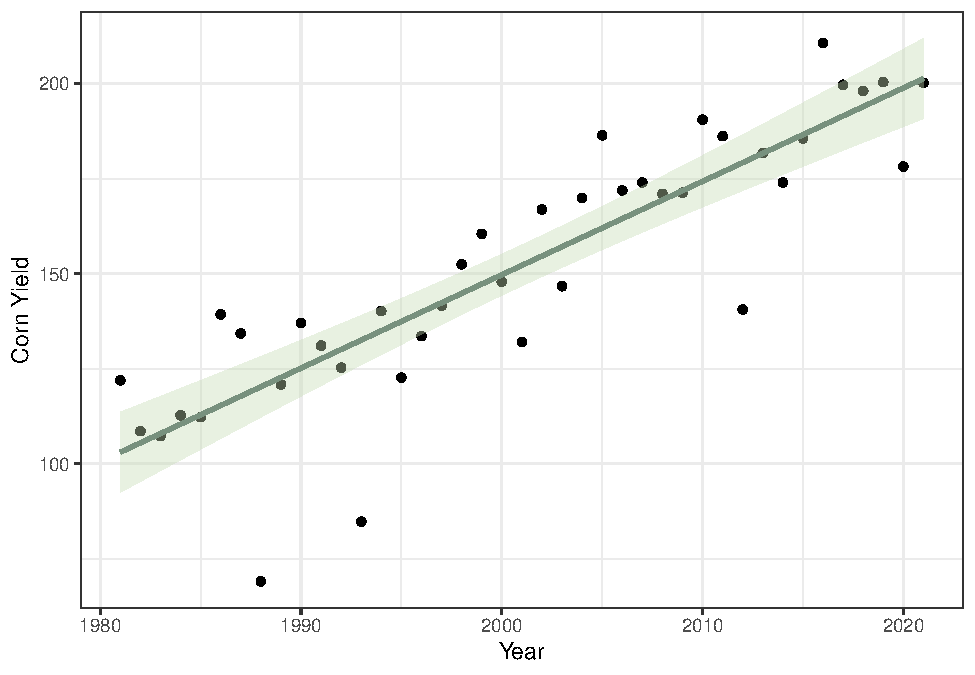
\includegraphics{Rportfolio-bookdown_files/figure-latex/unnamed-chunk-35-1.pdf}
\caption{\label{fig:unnamed-chunk-35}Linear regression of corn yields over time (years) in Winneshieck County, Iowa.}
\end{figure}

There is a significant positive correlation between corn yields and years in Winneshieck County, with an R-squared value of 0.755 and a P-value of 1.77e-13.

\hypertarget{fit-a-quadratic-time-trend-i.e.-year-year2-and-make-a-plot.-is-there-evidence-for-slowing-yield-growth}{%
\section{Fit a quadratic time trend (i.e., year + year\^{}2) and make a plot. Is there evidence for slowing yield growth?}\label{fit-a-quadratic-time-trend-i.e.-year-year2-and-make-a-plot.-is-there-evidence-for-slowing-yield-growth}}

\begin{Shaded}
\begin{Highlighting}[]
\NormalTok{winnecorn}\SpecialCharTok{$}\NormalTok{yearsq }\OtherTok{\textless{}{-}}\NormalTok{ winnecorn}\SpecialCharTok{$}\NormalTok{year}\SpecialCharTok{\^{}}\DecValTok{2} \CommentTok{\#square explanatory variables for quadratic}

\NormalTok{lm\_cornquad }\OtherTok{\textless{}{-}} \FunctionTok{lm}\NormalTok{(yield }\SpecialCharTok{\textasciitilde{}}\NormalTok{ year }\SpecialCharTok{+}\NormalTok{ yearsq, winnecorn)}
\FunctionTok{summary}\NormalTok{(lm\_cornquad)}
\end{Highlighting}
\end{Shaded}

\begin{verbatim}
## 
## Call:
## lm(formula = yield ~ year + yearsq, data = winnecorn)
## 
## Residuals:
##     Min      1Q  Median      3Q     Max 
## -51.384  -3.115   1.388   9.743  25.324 
## 
## Coefficients:
##               Estimate Std. Error t value Pr(>|t|)
## (Intercept)  2.583e+04  8.580e+04   0.301    0.765
## year        -2.812e+01  8.576e+01  -0.328    0.745
## yearsq       7.641e-03  2.143e-02   0.357    0.723
## 
## Residual standard error: 17.17 on 38 degrees of freedom
## Multiple R-squared:  0.7559, Adjusted R-squared:  0.7431 
## F-statistic: 58.84 on 2 and 38 DF,  p-value: 2.311e-12
\end{verbatim}

\begin{Shaded}
\begin{Highlighting}[]
\NormalTok{winnecorn}\SpecialCharTok{$}\NormalTok{y\_fitted }\OtherTok{\textless{}{-}}\NormalTok{ lm\_cornquad}\SpecialCharTok{$}\NormalTok{fitted.values}

\CommentTok{\#with the fitted values, create a non{-}linear trend}
\FunctionTok{ggplot}\NormalTok{(winnecorn) }\SpecialCharTok{+}
  \FunctionTok{geom\_point}\NormalTok{(}\AttributeTok{mapping =} \FunctionTok{aes}\NormalTok{(}\AttributeTok{x =}\NormalTok{ year, }\AttributeTok{y =}\NormalTok{ yield)) }\SpecialCharTok{+}
  \FunctionTok{geom\_line}\NormalTok{(}\AttributeTok{mapping =} \FunctionTok{aes}\NormalTok{(}\AttributeTok{x =}\NormalTok{ year, }\AttributeTok{y =}\NormalTok{ y\_fitted)) }\SpecialCharTok{+}
  \FunctionTok{theme\_bw}\NormalTok{() }\SpecialCharTok{+}
  \FunctionTok{labs}\NormalTok{(}\AttributeTok{x =} \StringTok{"Year"}\NormalTok{, }\AttributeTok{y =} \StringTok{"Corn Yield"}\NormalTok{)}
\end{Highlighting}
\end{Shaded}

\begin{figure}
\centering
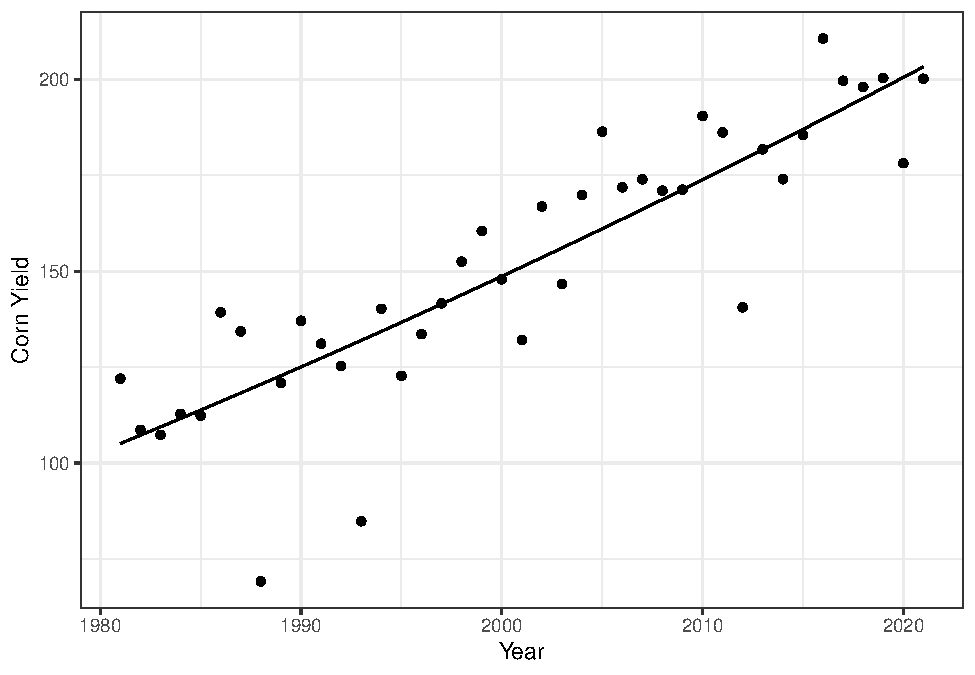
\includegraphics{Rportfolio-bookdown_files/figure-latex/unnamed-chunk-36-1.pdf}
\caption{\label{fig:unnamed-chunk-36}Quadratic fit of corn yields over time (years) in Winneshieck County, Iowa.}
\end{figure}

When we fit a quadratic line to the data, we find that it follows very closely to a linear regression, suggesting a fairly linear relationship between corn yields and years in Winneshieck County. There is no evidence of slowing yield growth in the model.

\hypertarget{time-series-lets-analyze-the-relationship-between-temperature-and-yields-for-the-winneshiek-county-time-series.-use-data-on-yield-and-summer-avg-tmax.-is-adding-year-or-tmax2-to-your-model-helpful-make-a-plot-and-interpret-the-results.}{%
\section{Time Series: Let's analyze the relationship between temperature and yields for the Winneshiek County time series. Use data on yield and summer avg Tmax. Is adding year or Tmax\^{}2 to your model helpful? Make a plot and interpret the results.}\label{time-series-lets-analyze-the-relationship-between-temperature-and-yields-for-the-winneshiek-county-time-series.-use-data-on-yield-and-summer-avg-tmax.-is-adding-year-or-tmax2-to-your-model-helpful-make-a-plot-and-interpret-the-results.}}

\begin{Shaded}
\begin{Highlighting}[]
\CommentTok{\# Winneshiek County summer temp maxes}
\NormalTok{tmaxdf}\SpecialCharTok{$}\NormalTok{doy }\OtherTok{\textless{}{-}} \FunctionTok{as.numeric}\NormalTok{(tmaxdf}\SpecialCharTok{$}\NormalTok{doy) }
\NormalTok{tmaxdf}\SpecialCharTok{$}\NormalTok{year }\OtherTok{\textless{}{-}} \FunctionTok{as.numeric}\NormalTok{(}\FunctionTok{as.character}\NormalTok{(tmaxdf}\SpecialCharTok{$}\NormalTok{year))}
\NormalTok{tmaxdf}\SpecialCharTok{$}\NormalTok{tmax }\OtherTok{\textless{}{-}} \FunctionTok{as.numeric}\NormalTok{(tmaxdf}\SpecialCharTok{$}\NormalTok{tmax)}

\NormalTok{winnesummer }\OtherTok{\textless{}{-}}\NormalTok{ tmaxdf }\SpecialCharTok{\%\textgreater{}\%}
  \FunctionTok{filter}\NormalTok{(countyfp}\SpecialCharTok{==}\DecValTok{191} \SpecialCharTok{\&}\NormalTok{ doy }\SpecialCharTok{\textgreater{}=} \DecValTok{152} \SpecialCharTok{\&}\NormalTok{ doy }\SpecialCharTok{\textless{}=} \DecValTok{243}\NormalTok{) }\SpecialCharTok{\%\textgreater{}\%} \CommentTok{\#day 152= June 1, 243= Aug 31}
  \FunctionTok{group\_by}\NormalTok{(year) }\SpecialCharTok{\%\textgreater{}\%}
  \FunctionTok{summarize}\NormalTok{(}\AttributeTok{meantmax =} \FunctionTok{mean}\NormalTok{(tmax))}

\NormalTok{lm\_summertmax }\OtherTok{\textless{}{-}} \FunctionTok{lm}\NormalTok{(meantmax }\SpecialCharTok{\textasciitilde{}}\NormalTok{ year, winnesummer)}
\FunctionTok{summary}\NormalTok{(lm\_summertmax) }\CommentTok{\#not sig}
\end{Highlighting}
\end{Shaded}

\begin{verbatim}
## 
## Call:
## lm(formula = meantmax ~ year, data = winnesummer)
## 
## Residuals:
##     Min      1Q  Median      3Q     Max 
## -2.5189 -0.7867 -0.0341  0.6859  3.7415 
## 
## Coefficients:
##             Estimate Std. Error t value Pr(>|t|)
## (Intercept) 41.57670   36.44848   1.141    0.262
## year        -0.00747    0.01823  -0.410    0.684
## 
## Residual standard error: 1.232 on 36 degrees of freedom
## Multiple R-squared:  0.004644,   Adjusted R-squared:  -0.02301 
## F-statistic: 0.168 on 1 and 36 DF,  p-value: 0.6844
\end{verbatim}

\begin{Shaded}
\begin{Highlighting}[]
\NormalTok{winnesummer}\SpecialCharTok{$}\NormalTok{yearsq }\OtherTok{\textless{}{-}}\NormalTok{ winnesummer}\SpecialCharTok{$}\NormalTok{year}\SpecialCharTok{\^{}}\DecValTok{2} \CommentTok{\#square explanatory variables for quadratic}
\NormalTok{winnesummer}\SpecialCharTok{$}\NormalTok{tmaxsq }\OtherTok{\textless{}{-}}\NormalTok{ winnesummer}\SpecialCharTok{$}\NormalTok{meantmax}\SpecialCharTok{\^{}}\DecValTok{2} 

\NormalTok{lm\_summerquad }\OtherTok{\textless{}{-}} \FunctionTok{lm}\NormalTok{(meantmax }\SpecialCharTok{\textasciitilde{}}\NormalTok{ year }\SpecialCharTok{+}\NormalTok{ yearsq, winnesummer)}
\FunctionTok{summary}\NormalTok{(lm\_summerquad)}
\end{Highlighting}
\end{Shaded}

\begin{verbatim}
## 
## Call:
## lm(formula = meantmax ~ year + yearsq, data = winnesummer)
## 
## Residuals:
##     Min      1Q  Median      3Q     Max 
## -2.4617 -0.8812 -0.0530  0.7204  3.7308 
## 
## Coefficients:
##               Estimate Std. Error t value Pr(>|t|)
## (Intercept)  3.618e+03  7.519e+03   0.481    0.633
## year        -3.585e+00  7.521e+00  -0.477    0.637
## yearsq       8.946e-04  1.881e-03   0.476    0.637
## 
## Residual standard error: 1.246 on 35 degrees of freedom
## Multiple R-squared:  0.01104,    Adjusted R-squared:  -0.04547 
## F-statistic: 0.1953 on 2 and 35 DF,  p-value: 0.8235
\end{verbatim}

\begin{Shaded}
\begin{Highlighting}[]
\NormalTok{winnesummer}\SpecialCharTok{$}\NormalTok{t\_fitted }\OtherTok{\textless{}{-}}\NormalTok{ lm\_summerquad}\SpecialCharTok{$}\NormalTok{fitted.values}

\CommentTok{\# Join yield and temp data}
\NormalTok{winne }\OtherTok{\textless{}{-}} \FunctionTok{inner\_join}\NormalTok{(winnecorn, winnesummer)}
\end{Highlighting}
\end{Shaded}

\begin{verbatim}
## Joining, by = c("year", "yearsq")
\end{verbatim}

\begin{Shaded}
\begin{Highlighting}[]
\NormalTok{lmwinne }\OtherTok{\textless{}{-}} \FunctionTok{lm}\NormalTok{(yield }\SpecialCharTok{\textasciitilde{}}\NormalTok{ yearsq }\SpecialCharTok{+}\NormalTok{ tmaxsq, }\AttributeTok{data =}\NormalTok{ winne)}
\FunctionTok{summary}\NormalTok{(lmwinne)}
\end{Highlighting}
\end{Shaded}

\begin{verbatim}
## 
## Call:
## lm(formula = yield ~ yearsq + tmaxsq, data = winne)
## 
## Residuals:
##     Min      1Q  Median      3Q     Max 
## -53.353  -7.496   2.089   9.806  27.874 
## 
## Coefficients:
##               Estimate Std. Error t value Pr(>|t|)    
## (Intercept) -2.314e+03  2.557e+02  -9.047 1.09e-10 ***
## yearsq       6.274e-04  6.295e-05   9.968 9.22e-12 ***
## tmaxsq      -6.445e-02  4.245e-02  -1.518    0.138    
## ---
## Signif. codes:  0 '***' 0.001 '**' 0.01 '*' 0.05 '.' 0.1 ' ' 1
## 
## Residual standard error: 16.97 on 35 degrees of freedom
## Multiple R-squared:  0.7492, Adjusted R-squared:  0.7349 
## F-statistic: 52.28 on 2 and 35 DF,  p-value: 3.074e-11
\end{verbatim}

\begin{Shaded}
\begin{Highlighting}[]
\NormalTok{winne}\SpecialCharTok{$}\NormalTok{allfit }\OtherTok{\textless{}{-}}\NormalTok{ lmwinne}\SpecialCharTok{$}\NormalTok{fitted.values}

\FunctionTok{ggplot}\NormalTok{(winne) }\SpecialCharTok{+}
  \FunctionTok{geom\_point}\NormalTok{(}\AttributeTok{mapping =} \FunctionTok{aes}\NormalTok{(}\AttributeTok{x =}\NormalTok{ year, }\AttributeTok{y =}\NormalTok{ yield)) }\SpecialCharTok{+}
  \FunctionTok{geom\_line}\NormalTok{(}\AttributeTok{mapping =} \FunctionTok{aes}\NormalTok{(}\AttributeTok{x =}\NormalTok{ year, }\AttributeTok{y =}\NormalTok{ allfit, }\AttributeTok{color=}\StringTok{"red"}\NormalTok{)) }\SpecialCharTok{+}
  \FunctionTok{geom\_line}\NormalTok{(}\AttributeTok{mapping =} \FunctionTok{aes}\NormalTok{(}\AttributeTok{x =}\NormalTok{ year, }\AttributeTok{y =}\NormalTok{ y\_fitted, }\AttributeTok{color=}\StringTok{"blue"}\NormalTok{)) }\SpecialCharTok{+}
  \FunctionTok{theme\_bw}\NormalTok{() }\SpecialCharTok{+}
  \FunctionTok{scale\_colour\_manual}\NormalTok{(}\AttributeTok{name =} \StringTok{"Model"}\NormalTok{, }
         \AttributeTok{values =}\FunctionTok{c}\NormalTok{(}\StringTok{"red"}\OtherTok{=}\StringTok{"red"}\NormalTok{,}\StringTok{"blue"}\OtherTok{=}\StringTok{"blue"}\NormalTok{), }\AttributeTok{labels =} \FunctionTok{c}\NormalTok{(}\StringTok{"Fit with Max Temp and Year"}\NormalTok{, }\StringTok{"Quadratic Yield Fit"}\NormalTok{)) }\SpecialCharTok{+}
  \FunctionTok{labs}\NormalTok{(}\AttributeTok{x =} \StringTok{"Year"}\NormalTok{, }\AttributeTok{y =} \StringTok{"Corn Yield"}\NormalTok{)}
\end{Highlighting}
\end{Shaded}

\begin{figure}
\centering
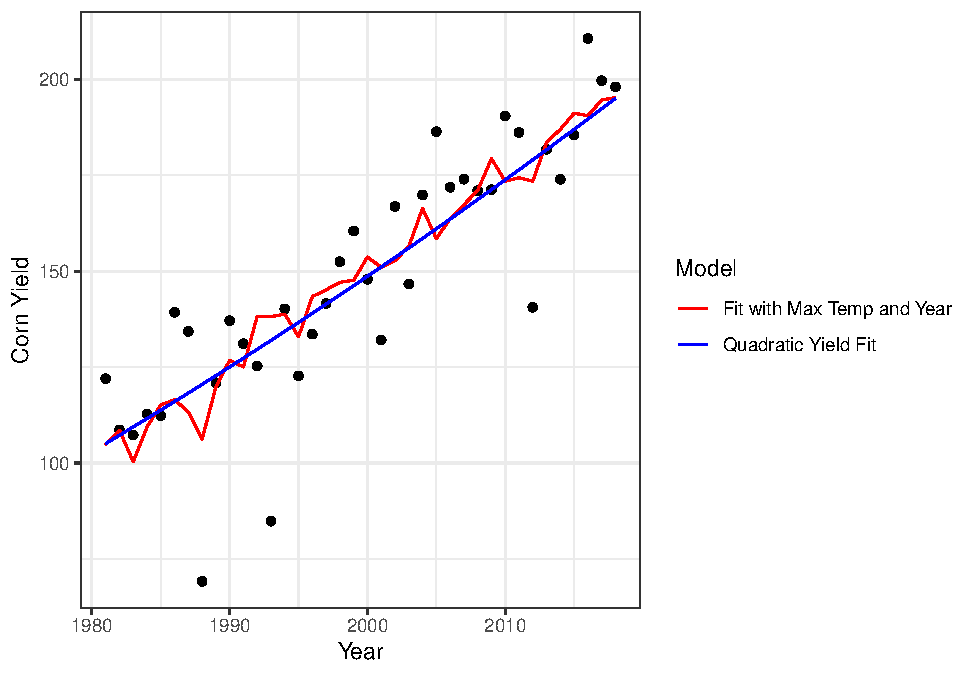
\includegraphics{Rportfolio-bookdown_files/figure-latex/unnamed-chunk-37-1.pdf}
\caption{\label{fig:unnamed-chunk-37}Comparative quadratic fit of corn yields over time (blue) and fitted line with maximum summer temperatures as well (red) in Winneshieck County, Iowa.}
\end{figure}

Adding maximum temperature trends to the model shows a similar trend, but peaks and dips in the fitted line highlight some of the outlying yield values and suggest an underlying relationship between maximum temperatures and yields. However, the relationship between squared maximum temperature and yield has a P-value of 0.14, compared with the year squared P-value of 9.22e-12, so it is clearly not the important driver of trends. This model has an R-squared value of 0.749, around the same as (slightly lower than) the simple linear regression model with only yield vs.~year. Thus, adding temperature doesn't significantly add to our understanding of yield trends in Winneshieck County.

\hypertarget{cross-section-analyze-the-relationship-between-temperature-and-yield-across-all-counties-in-2018.-is-there-a-relationship-interpret-the-results.}{%
\section{Cross-Section: Analyze the relationship between temperature and yield across all counties in 2018. Is there a relationship? Interpret the results.}\label{cross-section-analyze-the-relationship-between-temperature-and-yield-across-all-counties-in-2018.-is-there-a-relationship-interpret-the-results.}}

\begin{Shaded}
\begin{Highlighting}[]
\NormalTok{corn2018 }\OtherTok{\textless{}{-}}\NormalTok{ cornyields }\SpecialCharTok{\%\textgreater{}\%}
  \FunctionTok{filter}\NormalTok{(year }\SpecialCharTok{==} \StringTok{"2018"}\NormalTok{) }\SpecialCharTok{\%\textgreater{}\%}
  \FunctionTok{mutate\_at}\NormalTok{(}\FunctionTok{vars}\NormalTok{(county\_ansi), }\FunctionTok{funs}\NormalTok{(factor))}
  
\NormalTok{tmax2018 }\OtherTok{\textless{}{-}}\NormalTok{ tmaxdf }\SpecialCharTok{\%\textgreater{}\%}
  \FunctionTok{filter}\NormalTok{(year }\SpecialCharTok{==} \StringTok{"2018"}\NormalTok{) }\SpecialCharTok{\%\textgreater{}\%}
  \FunctionTok{filter}\NormalTok{(doy }\SpecialCharTok{\textgreater{}=} \DecValTok{152} \SpecialCharTok{\&}\NormalTok{ doy }\SpecialCharTok{\textless{}=} \DecValTok{243}\NormalTok{) }\SpecialCharTok{\%\textgreater{}\%}
  \FunctionTok{group\_by}\NormalTok{(countyfp) }\SpecialCharTok{\%\textgreater{}\%}
  \FunctionTok{rename}\NormalTok{(}\StringTok{"county\_ansi"} \OtherTok{=} \StringTok{"countyfp"}\NormalTok{) }\SpecialCharTok{\%\textgreater{}\%}
  \FunctionTok{summarize}\NormalTok{(}\AttributeTok{meantmax =} \FunctionTok{mean}\NormalTok{(tmax))}

\NormalTok{yieldtemp\_2018 }\OtherTok{\textless{}{-}} \FunctionTok{inner\_join}\NormalTok{(corn2018, tmax2018, }\AttributeTok{by=}\StringTok{"county\_ansi"}\NormalTok{) }\SpecialCharTok{\%\textgreater{}\%}
  \FunctionTok{mutate}\NormalTok{(}\AttributeTok{tmaxsq =}\NormalTok{ (meantmax}\SpecialCharTok{\^{}}\DecValTok{2}\NormalTok{))}

\NormalTok{yt\_lm }\OtherTok{\textless{}{-}} \FunctionTok{lm}\NormalTok{(yield }\SpecialCharTok{\textasciitilde{}}\NormalTok{ meantmax }\SpecialCharTok{+}\NormalTok{ tmaxsq, }\AttributeTok{data =}\NormalTok{ yieldtemp\_2018)}
\FunctionTok{summary}\NormalTok{(yt\_lm)}
\end{Highlighting}
\end{Shaded}

\begin{verbatim}
## 
## Call:
## lm(formula = yield ~ meantmax + tmaxsq, data = yieldtemp_2018)
## 
## Residuals:
##     Min      1Q  Median      3Q     Max 
## -44.221 -15.399   5.007  14.541  30.879 
## 
## Coefficients:
##              Estimate Std. Error t value Pr(>|t|)   
## (Intercept) -5501.602   1860.830  -2.957  0.00397 **
## meantmax      406.789    131.493   3.094  0.00263 **
## tmaxsq         -7.256      2.321  -3.126  0.00239 **
## ---
## Signif. codes:  0 '***' 0.001 '**' 0.01 '*' 0.05 '.' 0.1 ' ' 1
## 
## Residual standard error: 18.75 on 90 degrees of freedom
## Multiple R-squared:  0.1317, Adjusted R-squared:  0.1124 
## F-statistic: 6.827 on 2 and 90 DF,  p-value: 0.001736
\end{verbatim}

\begin{Shaded}
\begin{Highlighting}[]
\NormalTok{yieldtemp\_2018}\SpecialCharTok{$}\NormalTok{ytfit }\OtherTok{\textless{}{-}}\NormalTok{ yt\_lm}\SpecialCharTok{$}\NormalTok{fitted.values}

\FunctionTok{ggplot}\NormalTok{(yieldtemp\_2018) }\SpecialCharTok{+}
  \FunctionTok{geom\_point}\NormalTok{(}\AttributeTok{mapping =} \FunctionTok{aes}\NormalTok{(}\AttributeTok{x =}\NormalTok{ meantmax, }\AttributeTok{y =}\NormalTok{ yield)) }\SpecialCharTok{+}
  \FunctionTok{geom\_line}\NormalTok{(}\AttributeTok{mapping =} \FunctionTok{aes}\NormalTok{(}\AttributeTok{x =}\NormalTok{ meantmax, }\AttributeTok{y =}\NormalTok{ ytfit, }\AttributeTok{color=}\StringTok{"red"}\NormalTok{)) }\SpecialCharTok{+}
  \FunctionTok{theme\_bw}\NormalTok{() }\SpecialCharTok{+} \FunctionTok{theme}\NormalTok{(}\AttributeTok{legend.position=}\StringTok{"none"}\NormalTok{) }\SpecialCharTok{+}
  \FunctionTok{labs}\NormalTok{(}\AttributeTok{x =} \StringTok{"Mean Max Temperature (C)"}\NormalTok{, }\AttributeTok{y =} \StringTok{"Corn Yield"}\NormalTok{)}
\end{Highlighting}
\end{Shaded}

\begin{figure}
\centering
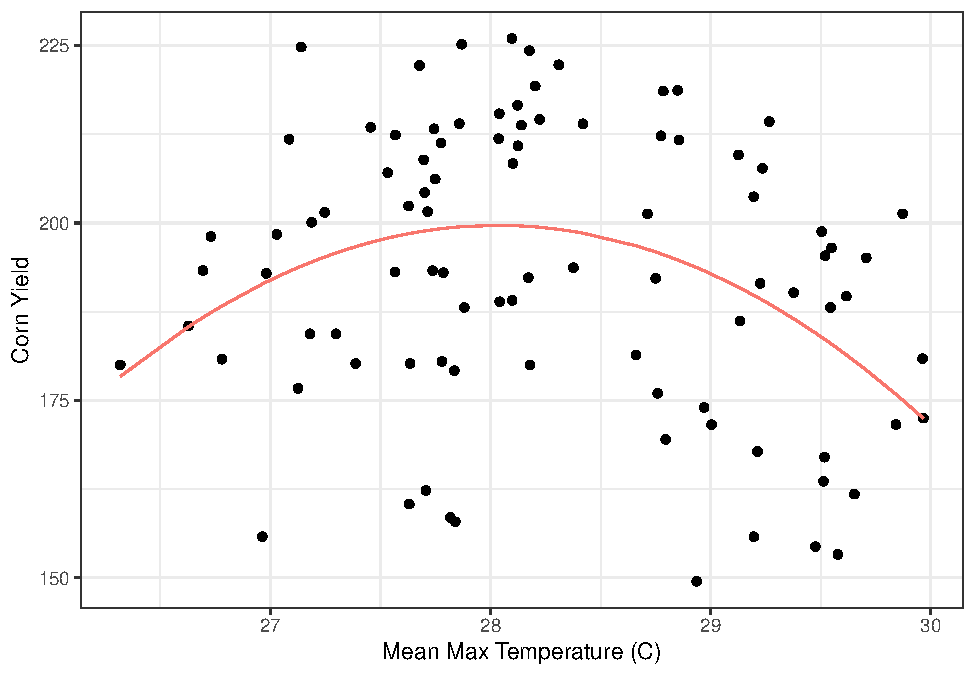
\includegraphics{Rportfolio-bookdown_files/figure-latex/unnamed-chunk-38-1.pdf}
\caption{\label{fig:unnamed-chunk-38}Quadratic fit of corn yields versus maximum summer temperatures (Degrees C) across Iowa.}
\end{figure}

There is a clear relationship with maximum temperatures and corn yields demonstrated in Figure 4. As we might expect, there appears to be a ``sweet spot'' in regard to temperature, with corn crops performing best at moderate temperatures and yields falling off at both low and high temperature years. Lower mean maximum temperatures may indicate even lower temperatures that can shock crops, and high means are likely to cause high evaporation and withering. P\textless0.003 for the relationship between temperature and corn yield across Iowa.

\hypertarget{panel-one-way-to-leverage-multiple-time-series-is-to-group-all-data-into-what-is-called-a-panel-regression.-convert-the-county-id-code-countyfp-or-county_ansi-into-factor-using-as.factor-then-include-this-variable-in-a-regression-using-all-counties-yield-and-summer-temperature-data.-how-does-the-significance-of-your-temperature-coefficients-tmax-tmax2-change-make-a-plot-comparing-actual-and-fitted-yields-and-interpret-the-results-of-your-model.}{%
\section{Panel: One way to leverage multiple time series is to group all data into what is called a ``panel'' regression. Convert the county ID code (``countyfp'' or ``county\_ansi'') into factor using as.factor, then include this variable in a regression using all counties' yield and summer temperature data. How does the significance of your temperature coefficients (Tmax, Tmax\^{}2) change? Make a plot comparing actual and fitted yields and interpret the results of your model.}\label{panel-one-way-to-leverage-multiple-time-series-is-to-group-all-data-into-what-is-called-a-panel-regression.-convert-the-county-id-code-countyfp-or-county_ansi-into-factor-using-as.factor-then-include-this-variable-in-a-regression-using-all-counties-yield-and-summer-temperature-data.-how-does-the-significance-of-your-temperature-coefficients-tmax-tmax2-change-make-a-plot-comparing-actual-and-fitted-yields-and-interpret-the-results-of-your-model.}}

\begin{Shaded}
\begin{Highlighting}[]
\NormalTok{corn\_all }\OtherTok{\textless{}{-}}\NormalTok{ cornyields }\SpecialCharTok{\%\textgreater{}\%}
  \FunctionTok{mutate\_at}\NormalTok{(}\FunctionTok{vars}\NormalTok{(county\_ansi), }\FunctionTok{funs}\NormalTok{(factor))}
  
\NormalTok{tmax\_all }\OtherTok{\textless{}{-}}\NormalTok{ tmaxdf }\SpecialCharTok{\%\textgreater{}\%}
  \FunctionTok{filter}\NormalTok{(doy }\SpecialCharTok{\textgreater{}=} \DecValTok{152} \SpecialCharTok{\&}\NormalTok{ doy }\SpecialCharTok{\textless{}=} \DecValTok{243}\NormalTok{) }\SpecialCharTok{\%\textgreater{}\%}
  \FunctionTok{group\_by}\NormalTok{(countyfp, year) }\SpecialCharTok{\%\textgreater{}\%}
  \FunctionTok{rename}\NormalTok{(}\StringTok{"county\_ansi"} \OtherTok{=} \StringTok{"countyfp"}\NormalTok{) }\SpecialCharTok{\%\textgreater{}\%}
  \FunctionTok{summarize}\NormalTok{(}\AttributeTok{meantmax =} \FunctionTok{mean}\NormalTok{(tmax))}
\end{Highlighting}
\end{Shaded}

\begin{verbatim}
## `summarise()` has grouped output by 'county_ansi'. You can override using the
## `.groups` argument.
\end{verbatim}

\begin{Shaded}
\begin{Highlighting}[]
\NormalTok{yieldtemp\_all }\OtherTok{\textless{}{-}} \FunctionTok{inner\_join}\NormalTok{(corn\_all, tmax\_all) }\SpecialCharTok{\%\textgreater{}\%}
  \FunctionTok{mutate}\NormalTok{(}\AttributeTok{tmaxsq =}\NormalTok{ (meantmax}\SpecialCharTok{\^{}}\DecValTok{2}\NormalTok{)) }\SpecialCharTok{\%\textgreater{}\%}
  \FunctionTok{mutate}\NormalTok{(}\AttributeTok{yearsq =}\NormalTok{ year}\SpecialCharTok{\^{}}\DecValTok{2}\NormalTok{)}
\end{Highlighting}
\end{Shaded}

\begin{verbatim}
## Joining, by = c("county_ansi", "year")
\end{verbatim}

\begin{Shaded}
\begin{Highlighting}[]
\NormalTok{ytc\_lm }\OtherTok{\textless{}{-}} \FunctionTok{lm}\NormalTok{(yield }\SpecialCharTok{\textasciitilde{}}\NormalTok{ year }\SpecialCharTok{+}\NormalTok{ meantmax }\SpecialCharTok{+}\NormalTok{ tmaxsq }\SpecialCharTok{+}\NormalTok{ county\_ansi, }\AttributeTok{data =}\NormalTok{ yieldtemp\_all)}
\FunctionTok{summary}\NormalTok{(ytc\_lm)}
\end{Highlighting}
\end{Shaded}

\begin{verbatim}
## 
## Call:
## lm(formula = yield ~ year + meantmax + tmaxsq + county_ansi, 
##     data = yieldtemp_all)
## 
## Residuals:
##     Min      1Q  Median      3Q     Max 
## -81.645  -9.720   1.924  13.232  40.409 
## 
## Coefficients:
##                  Estimate Std. Error t value Pr(>|t|)    
## (Intercept)    -5.826e+03  9.804e+01 -59.431  < 2e-16 ***
## year            2.203e+00  2.836e-02  77.664  < 2e-16 ***
## meantmax        1.182e+02  6.108e+00  19.352  < 2e-16 ***
## tmaxsq         -2.225e+00  1.085e-01 -20.503  < 2e-16 ***
## county_ansi3   -4.527e+00  4.321e+00  -1.048 0.294839    
## county_ansi5    2.716e+00  4.343e+00   0.625 0.531743    
## county_ansi7   -1.828e+01  4.350e+00  -4.203 2.70e-05 ***
## county_ansi9    5.068e+00  4.323e+00   1.172 0.241144    
## county_ansi11   7.186e+00  4.325e+00   1.661 0.096732 .  
## county_ansi13   7.289e+00  4.329e+00   1.684 0.092303 .  
## county_ansi15   1.498e+01  4.323e+00   3.466 0.000534 ***
## county_ansi17   1.133e+01  4.332e+00   2.615 0.008966 ** 
## county_ansi19   7.651e+00  4.334e+00   1.765 0.077577 .  
## county_ansi21   8.640e+00  4.328e+00   1.996 0.045974 *  
## county_ansi23   9.089e+00  4.327e+00   2.100 0.035779 *  
## county_ansi25   1.039e+01  4.326e+00   2.401 0.016400 *  
## county_ansi27   9.666e+00  4.323e+00   2.236 0.025421 *  
## county_ansi29   6.145e+00  4.321e+00   1.422 0.155092    
## county_ansi31   1.579e+01  4.324e+00   3.651 0.000264 ***
## county_ansi33   4.582e+00  4.338e+00   1.056 0.290980    
## county_ansi35   1.390e+01  4.325e+00   3.213 0.001325 ** 
## county_ansi37   2.169e+00  4.341e+00   0.500 0.617274    
## county_ansi39  -2.404e+01  4.350e+00  -5.527 3.48e-08 ***
## county_ansi41   6.611e+00  4.329e+00   1.527 0.126809    
## county_ansi43   8.864e+00  4.337e+00   2.044 0.041033 *  
## county_ansi45   1.055e+01  4.325e+00   2.439 0.014756 *  
## county_ansi47   6.528e+00  4.324e+00   1.510 0.131221    
## county_ansi49   1.081e+01  4.321e+00   2.502 0.012386 *  
## county_ansi51  -1.457e+01  4.352e+00  -3.349 0.000820 ***
## county_ansi53  -1.603e+01  4.350e+00  -3.686 0.000232 ***
## county_ansi55   9.423e+00  4.338e+00   2.172 0.029916 *  
## county_ansi57   1.050e+01  4.321e+00   2.429 0.015186 *  
## county_ansi59   2.906e+00  4.336e+00   0.670 0.502836    
## county_ansi61   9.795e+00  4.340e+00   2.257 0.024059 *  
## county_ansi63   7.232e+00  4.340e+00   1.666 0.095754 .  
## county_ansi65   7.319e+00  4.341e+00   1.686 0.091905 .  
## county_ansi67   4.791e+00  4.334e+00   1.106 0.269008    
## county_ansi69   1.131e+01  4.330e+00   2.612 0.009035 ** 
## county_ansi71   1.358e+01  4.330e+00   3.136 0.001726 ** 
## county_ansi73   1.462e+01  4.321e+00   3.382 0.000727 ***
## county_ansi75   1.151e+01  4.328e+00   2.659 0.007863 ** 
## county_ansi77   3.379e+00  4.321e+00   0.782 0.434297    
## county_ansi79   1.315e+01  4.324e+00   3.042 0.002370 ** 
## county_ansi81   8.706e+00  4.340e+00   2.006 0.044917 *  
## county_ansi83   1.395e+01  4.326e+00   3.225 0.001271 ** 
## county_ansi85   6.891e+00  4.321e+00   1.595 0.110834    
## county_ansi87   5.280e+00  4.321e+00   1.222 0.221864    
## county_ansi89   9.433e-01  4.364e+00   0.216 0.828875    
## county_ansi91   9.881e+00  4.334e+00   2.280 0.022661 *  
## county_ansi93   1.186e+01  4.325e+00   2.743 0.006124 ** 
## county_ansi95   7.214e+00  4.322e+00   1.669 0.095161 .  
## county_ansi97  -1.386e+00  4.330e+00  -0.320 0.748823    
## county_ansi99   1.440e+01  4.322e+00   3.332 0.000871 ***
## county_ansi101  5.352e-01  4.325e+00   0.124 0.901510    
## county_ansi103  4.380e+00  4.322e+00   1.013 0.310971    
## county_ansi105  7.730e+00  4.328e+00   1.786 0.074158 .  
## county_ansi107  2.203e+00  4.321e+00   0.510 0.610224    
## county_ansi109  1.222e+01  4.335e+00   2.819 0.004839 ** 
## county_ansi111  1.779e+00  4.324e+00   0.411 0.680740    
## county_ansi113  6.415e+00  4.326e+00   1.483 0.138218    
## county_ansi115  7.330e+00  4.322e+00   1.696 0.089966 .  
## county_ansi117 -2.168e+01  4.381e+00  -4.949 7.81e-07 ***
## county_ansi119  9.328e+00  4.325e+00   2.157 0.031063 *  
## county_ansi121 -2.587e+00  4.321e+00  -0.599 0.549390    
## county_ansi123  8.152e+00  4.321e+00   1.887 0.059302 .  
## county_ansi125  1.919e+00  4.321e+00   0.444 0.656948    
## county_ansi127  1.418e+01  4.326e+00   3.278 0.001055 ** 
## county_ansi129  1.023e+01  4.385e+00   2.332 0.019741 *  
## county_ansi131  7.285e+00  4.352e+00   1.674 0.094242 .  
## county_ansi133  7.987e-01  4.321e+00   0.185 0.853378    
## county_ansi135 -1.585e+01  4.350e+00  -3.643 0.000273 ***
## county_ansi137  5.885e+00  4.322e+00   1.362 0.173381    
## county_ansi139  8.283e+00  4.321e+00   1.917 0.055337 .  
## county_ansi141  1.423e+01  4.328e+00   3.288 0.001018 ** 
## county_ansi143  8.743e+00  4.337e+00   2.016 0.043890 *  
## county_ansi145 -3.674e-01  4.322e+00  -0.085 0.932261    
## county_ansi147  7.261e+00  4.330e+00   1.677 0.093601 .  
## county_ansi149  7.352e+00  4.322e+00   1.701 0.089007 .  
## county_ansi151  1.150e+01  4.326e+00   2.659 0.007880 ** 
## county_ansi153  1.403e+01  4.321e+00   3.247 0.001178 ** 
## county_ansi155  1.127e+01  4.350e+00   2.590 0.009627 ** 
## county_ansi157  1.055e+01  4.322e+00   2.441 0.014702 *  
## county_ansi159 -2.070e+01  4.321e+00  -4.792 1.72e-06 ***
## county_ansi161  9.390e+00  4.326e+00   2.170 0.030050 *  
## county_ansi163  1.628e+01  4.323e+00   3.765 0.000169 ***
## county_ansi165  7.673e+00  4.323e+00   1.775 0.075966 .  
## county_ansi167  1.558e+01  4.323e+00   3.603 0.000318 ***
## county_ansi169  1.122e+01  4.325e+00   2.593 0.009543 ** 
## county_ansi171  9.740e+00  4.325e+00   2.252 0.024387 *  
## county_ansi173 -1.404e+01  4.350e+00  -3.228 0.001256 ** 
## county_ansi175 -1.155e+01  4.350e+00  -2.655 0.007967 ** 
## county_ansi177 -5.278e+00  4.329e+00  -1.219 0.222881    
## county_ansi179 -3.220e+00  4.351e+00  -0.740 0.459267    
## county_ansi181 -2.159e+00  4.321e+00  -0.500 0.617309    
## county_ansi183  1.042e+01  4.321e+00   2.410 0.015981 *  
## county_ansi185 -2.189e+01  4.350e+00  -5.033 5.07e-07 ***
## county_ansi187  1.421e+01  4.326e+00   3.285 0.001029 ** 
## county_ansi189  8.236e+00  4.344e+00   1.896 0.058035 .  
## county_ansi191  4.567e+00  4.350e+00   1.050 0.293826    
## county_ansi193  2.799e+00  4.321e+00   0.648 0.517252    
## county_ansi195  6.123e+00  4.356e+00   1.406 0.159892    
## county_ansi197  1.156e+01  4.329e+00   2.669 0.007634 ** 
## ---
## Signif. codes:  0 '***' 0.001 '**' 0.01 '*' 0.05 '.' 0.1 ' ' 1
## 
## Residual standard error: 18.83 on 3646 degrees of freedom
## Multiple R-squared:  0.7207, Adjusted R-squared:  0.7129 
## F-statistic: 93.13 on 101 and 3646 DF,  p-value: < 2.2e-16
\end{verbatim}

\begin{Shaded}
\begin{Highlighting}[]
\NormalTok{yieldtemp\_all}\SpecialCharTok{$}\NormalTok{fittedyield }\OtherTok{\textless{}{-}}\NormalTok{ ytc\_lm}\SpecialCharTok{$}\NormalTok{fitted.values}

\FunctionTok{ggplot}\NormalTok{(yieldtemp\_all, }\AttributeTok{mapping =} \FunctionTok{aes}\NormalTok{(}\AttributeTok{x =}\NormalTok{ fittedyield, }\AttributeTok{y =}\NormalTok{ yield)) }\SpecialCharTok{+}
  \FunctionTok{geom\_point}\NormalTok{() }\SpecialCharTok{+}
  \FunctionTok{geom\_smooth}\NormalTok{(}\AttributeTok{method=}\StringTok{"lm"}\NormalTok{) }\SpecialCharTok{+}
  \FunctionTok{theme\_bw}\NormalTok{() }\SpecialCharTok{+} \FunctionTok{theme}\NormalTok{(}\AttributeTok{legend.position=}\StringTok{"none"}\NormalTok{) }\SpecialCharTok{+}
  \FunctionTok{labs}\NormalTok{(}\AttributeTok{x =} \StringTok{"Fitted Yield"}\NormalTok{, }\AttributeTok{y =} \StringTok{"Actual Yield"}\NormalTok{)}
\end{Highlighting}
\end{Shaded}

\begin{verbatim}
## `geom_smooth()` using formula 'y ~ x'
\end{verbatim}

\begin{figure}
\centering
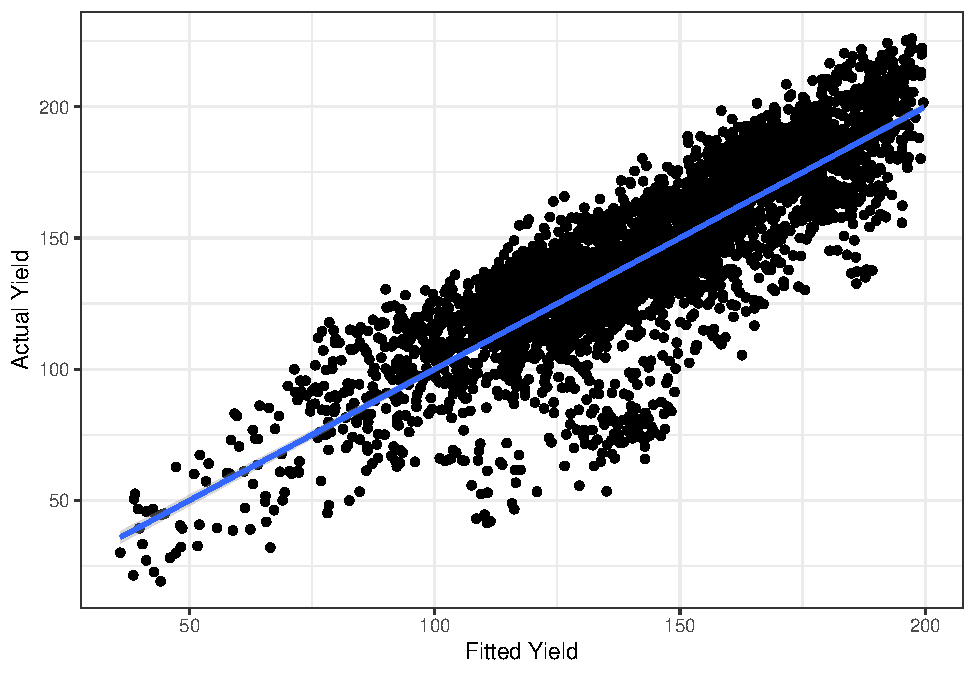
\includegraphics{Rportfolio-bookdown_files/figure-latex/unnamed-chunk-39-1.pdf}
\caption{\label{fig:unnamed-chunk-39}Fitted model yield values versus actual yield values for all counties of Iowa over all available years, from 1981 to 2018.}
\end{figure}

\begin{Shaded}
\begin{Highlighting}[]
\FunctionTok{par}\NormalTok{(}\AttributeTok{mfrow=}\FunctionTok{c}\NormalTok{(}\DecValTok{2}\NormalTok{,}\DecValTok{2}\NormalTok{))}
\FunctionTok{plot}\NormalTok{(ytc\_lm)}
\end{Highlighting}
\end{Shaded}

\begin{figure}
\centering
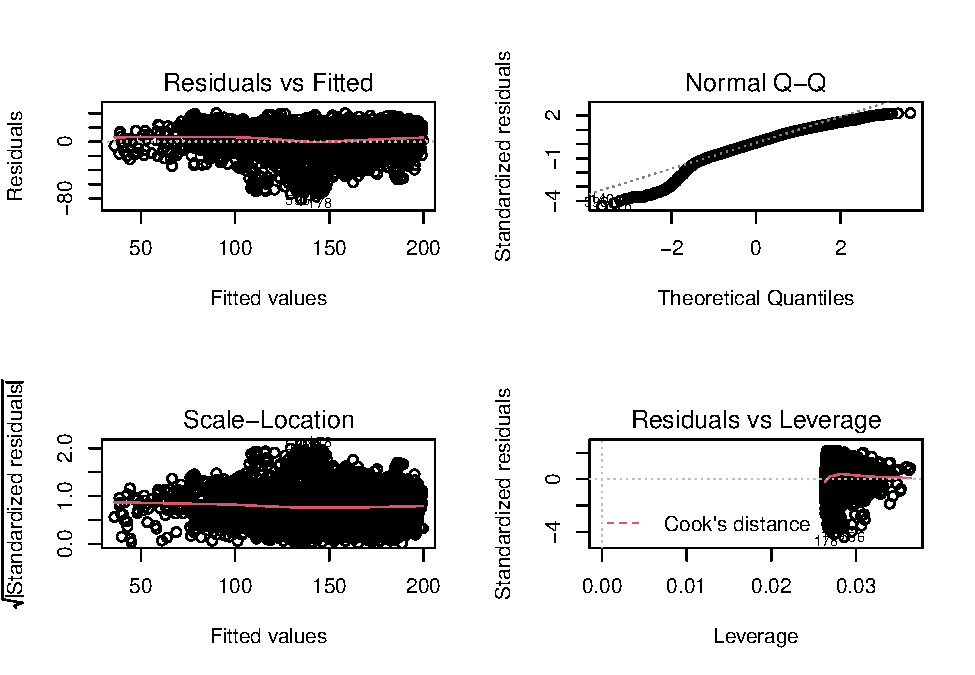
\includegraphics{Rportfolio-bookdown_files/figure-latex/unnamed-chunk-40-1.pdf}
\caption{\label{fig:unnamed-chunk-40}Residuals (top left), Normal Q-Q (top right), Scale-Location (bottom left), and Cook's Distance (bottom right) plots for the panel regression model.}
\end{figure}

As a panel regression of all counties over all years, the statistical significance of year, mean maximum temperature, and squared maximum temperature as predictors of yield becomes stronger (P\textless2e-16 for each). The R squared value for the model is 0.721, indicating a pretty good fit, as is evident in Figure 5. However, the residuals for the model are pretty wide (Figures 5, 6) and the data may not be very normally distributed (Figure 6).

\hypertarget{soybeans-download-nass-data-on-soybean-yields-and-explore-either-a-time-series-relationship-for-a-given-county-the-cross-sectional-relationship-for-a-given-year-or-a-panel-across-all-counties-and-years.}{%
\section{Soybeans: Download NASS data on soybean yields and explore either a time series relationship for a given county, the cross-sectional relationship for a given year, or a panel across all counties and years.}\label{soybeans-download-nass-data-on-soybean-yields-and-explore-either-a-time-series-relationship-for-a-given-county-the-cross-sectional-relationship-for-a-given-year-or-a-panel-across-all-counties-and-years.}}

\begin{Shaded}
\begin{Highlighting}[]
\CommentTok{\# parameters to query on }
\NormalTok{params2 }\OtherTok{\textless{}{-}} \FunctionTok{list}\NormalTok{(}\AttributeTok{commodity\_desc =} \StringTok{"SOYBEANS"}\NormalTok{, }\AttributeTok{prodn\_practice\_desc =} \StringTok{"ALL PRODUCTION PRACTICES"}\NormalTok{, }\AttributeTok{year\_\_GE =} \DecValTok{1981}\NormalTok{, }\AttributeTok{state\_alpha =} \StringTok{"IA"}\NormalTok{)}

\CommentTok{\# download}
\NormalTok{soyyieldsall }\OtherTok{\textless{}{-}} \FunctionTok{nassqs\_yields}\NormalTok{(params)}
\end{Highlighting}
\end{Shaded}

\begin{verbatim}
##   |                                                                              |                                                                      |   0%  |                                                                              |=                                                                     |   1%  |                                                                              |=                                                                     |   2%  |                                                                              |==                                                                    |   2%  |                                                                              |==                                                                    |   3%  |                                                                              |==                                                                    |   4%  |                                                                              |===                                                                   |   4%  |                                                                              |===                                                                   |   5%  |                                                                              |====                                                                  |   5%  |                                                                              |====                                                                  |   6%  |                                                                              |=====                                                                 |   7%  |                                                                              |=====                                                                 |   8%  |                                                                              |======                                                                |   8%  |                                                                              |======                                                                |   9%  |                                                                              |=======                                                               |   9%  |                                                                              |=======                                                               |  10%  |                                                                              |=======                                                               |  11%  |                                                                              |========                                                              |  11%  |                                                                              |========                                                              |  12%  |                                                                              |=========                                                             |  12%  |                                                                              |=========                                                             |  13%  |                                                                              |==========                                                            |  14%  |                                                                              |==========                                                            |  15%  |                                                                              |===========                                                           |  15%  |                                                                              |===========                                                           |  16%  |                                                                              |============                                                          |  17%  |                                                                              |============                                                          |  18%  |                                                                              |=============                                                         |  18%  |                                                                              |=============                                                         |  19%  |                                                                              |==============                                                        |  19%  |                                                                              |==============                                                        |  20%  |                                                                              |==============                                                        |  21%  |                                                                              |===============                                                       |  21%  |                                                                              |===============                                                       |  22%  |                                                                              |================                                                      |  22%  |                                                                              |================                                                      |  23%  |                                                                              |=================                                                     |  24%  |                                                                              |=================                                                     |  25%  |                                                                              |==================                                                    |  25%  |                                                                              |==================                                                    |  26%  |                                                                              |===================                                                   |  27%  |                                                                              |===================                                                   |  28%  |                                                                              |====================                                                  |  28%  |                                                                              |====================                                                  |  29%  |                                                                              |=====================                                                 |  30%  |                                                                              |=====================                                                 |  31%  |                                                                              |======================                                                |  31%  |                                                                              |======================                                                |  32%  |                                                                              |=======================                                               |  32%  |                                                                              |=======================                                               |  33%  |                                                                              |========================                                              |  34%  |                                                                              |========================                                              |  35%  |                                                                              |=========================                                             |  35%  |                                                                              |=========================                                             |  36%  |                                                                              |==========================                                            |  37%  |                                                                              |==========================                                            |  38%  |                                                                              |===========================                                           |  38%  |                                                                              |===========================                                           |  39%  |                                                                              |============================                                          |  39%  |                                                                              |============================                                          |  40%  |                                                                              |=============================                                         |  41%  |                                                                              |=============================                                         |  42%  |                                                                              |==============================                                        |  42%  |                                                                              |==============================                                        |  43%  |                                                                              |===============================                                       |  44%  |                                                                              |===============================                                       |  45%  |                                                                              |================================                                      |  45%  |                                                                              |================================                                      |  46%  |                                                                              |=================================                                     |  47%  |                                                                              |=================================                                     |  48%  |                                                                              |==================================                                    |  48%  |                                                                              |==================================                                    |  49%  |                                                                              |===================================                                   |  49%  |                                                                              |===================================                                   |  50%  |                                                                              |====================================                                  |  51%  |                                                                              |====================================                                  |  52%  |                                                                              |=====================================                                 |  52%  |                                                                              |=====================================                                 |  53%  |                                                                              |=====================================                                 |  54%  |                                                                              |======================================                                |  54%  |                                                                              |======================================                                |  55%  |                                                                              |=======================================                               |  55%  |                                                                              |=======================================                               |  56%  |                                                                              |========================================                              |  57%  |                                                                              |========================================                              |  58%  |                                                                              |=========================================                             |  58%  |                                                                              |=========================================                             |  59%  |                                                                              |==========================================                            |  59%  |                                                                              |==========================================                            |  60%  |                                                                              |==========================================                            |  61%  |                                                                              |===========================================                           |  61%  |                                                                              |===========================================                           |  62%  |                                                                              |============================================                          |  62%  |                                                                              |============================================                          |  63%  |                                                                              |=============================================                         |  64%  |                                                                              |=============================================                         |  65%  |                                                                              |==============================================                        |  65%  |                                                                              |==============================================                        |  66%  |                                                                              |===============================================                       |  67%  |                                                                              |===============================================                       |  68%  |                                                                              |================================================                      |  68%  |                                                                              |================================================                      |  69%  |                                                                              |=================================================                     |  69%  |                                                                              |=================================================                     |  70%  |                                                                              |=================================================                     |  71%  |                                                                              |==================================================                    |  71%  |                                                                              |==================================================                    |  72%  |                                                                              |===================================================                   |  72%  |                                                                              |===================================================                   |  73%  |                                                                              |====================================================                  |  74%  |                                                                              |====================================================                  |  75%  |                                                                              |=====================================================                 |  75%  |                                                                              |=====================================================                 |  76%  |                                                                              |======================================================                |  76%  |                                                                              |======================================================                |  77%  |                                                                              |======================================================                |  78%  |                                                                              |=======================================================               |  78%  |                                                                              |=======================================================               |  79%  |                                                                              |========================================================              |  80%  |                                                                              |=========================================================             |  81%  |                                                                              |=========================================================             |  82%  |                                                                              |==========================================================            |  82%  |                                                                              |==========================================================            |  83%  |                                                                              |===========================================================           |  84%  |                                                                              |===========================================================           |  85%  |                                                                              |============================================================          |  85%  |                                                                              |============================================================          |  86%  |                                                                              |=============================================================         |  86%  |                                                                              |=============================================================         |  87%  |                                                                              |=============================================================         |  88%  |                                                                              |==============================================================        |  88%  |                                                                              |==============================================================        |  89%  |                                                                              |===============================================================       |  90%  |                                                                              |================================================================      |  91%  |                                                                              |================================================================      |  92%  |                                                                              |=================================================================     |  92%  |                                                                              |=================================================================     |  93%  |                                                                              |=================================================================     |  94%  |                                                                              |==================================================================    |  94%  |                                                                              |==================================================================    |  95%  |                                                                              |===================================================================   |  95%  |                                                                              |===================================================================   |  96%  |                                                                              |====================================================================  |  96%  |                                                                              |====================================================================  |  97%  |                                                                              |====================================================================  |  98%  |                                                                              |===================================================================== |  98%  |                                                                              |===================================================================== |  99%  |                                                                              |======================================================================| 100%
\end{verbatim}

\begin{Shaded}
\begin{Highlighting}[]
\NormalTok{soyyieldsall}\SpecialCharTok{$}\NormalTok{county\_ansi }\OtherTok{\textless{}{-}} \FunctionTok{as.numeric}\NormalTok{(soyyieldsall}\SpecialCharTok{$}\NormalTok{county\_ansi)}
\NormalTok{soyyieldsall}\SpecialCharTok{$}\NormalTok{yield }\OtherTok{\textless{}{-}} \FunctionTok{as.numeric}\NormalTok{(soyyieldsall}\SpecialCharTok{$}\NormalTok{Value)}

\CommentTok{\# clean and filter this dataset}
\NormalTok{soy }\OtherTok{\textless{}{-}} \FunctionTok{select}\NormalTok{(soyyieldsall, county\_ansi, county\_name, yield, year) }\SpecialCharTok{\%\textgreater{}\%}
  \FunctionTok{filter}\NormalTok{(}\SpecialCharTok{!}\FunctionTok{is.na}\NormalTok{(county\_ansi) }\SpecialCharTok{\&} \SpecialCharTok{!}\FunctionTok{is.na}\NormalTok{(yield))}
\NormalTok{soy }\OtherTok{\textless{}{-}} \FunctionTok{tibble}\NormalTok{(soy)}

\NormalTok{soy\_panel }\OtherTok{\textless{}{-}}\NormalTok{ soy }\SpecialCharTok{\%\textgreater{}\%}
  \FunctionTok{mutate\_at}\NormalTok{(}\FunctionTok{vars}\NormalTok{(county\_ansi), }\FunctionTok{funs}\NormalTok{(factor)) }\SpecialCharTok{\%\textgreater{}\%}
  \FunctionTok{mutate}\NormalTok{(}\AttributeTok{yearsq =}\NormalTok{ year}\SpecialCharTok{\^{}}\DecValTok{2}\NormalTok{)}

\NormalTok{soypanel\_lm }\OtherTok{\textless{}{-}} \FunctionTok{lm}\NormalTok{(yield }\SpecialCharTok{\textasciitilde{}}\NormalTok{ year }\SpecialCharTok{+}\NormalTok{ yearsq }\SpecialCharTok{+}\NormalTok{ county\_ansi, }\AttributeTok{data =}\NormalTok{ soy\_panel)}
\FunctionTok{summary}\NormalTok{(soypanel\_lm)}
\end{Highlighting}
\end{Shaded}

\begin{verbatim}
## 
## Call:
## lm(formula = yield ~ year + yearsq + county_ansi, data = soy_panel)
## 
## Residuals:
##      Min       1Q   Median       3Q      Max 
## -100.865   -9.428    3.328   14.357   54.326 
## 
## Coefficients:
##                  Estimate Std. Error t value Pr(>|t|)    
## (Intercept)     4.646e+04  1.090e+04   4.263 2.06e-05 ***
## year           -4.859e+01  1.089e+01  -4.461 8.38e-06 ***
## yearsq          1.272e-02  2.722e-03   4.672 3.09e-06 ***
## county_ansi3   -3.974e+00  4.809e+00  -0.826 0.408591    
## county_ansi5    1.128e+01  4.749e+00   2.376 0.017550 *  
## county_ansi7   -1.878e+01  4.778e+00  -3.931 8.61e-05 ***
## county_ansi9    9.877e+00  4.749e+00   2.080 0.037621 *  
## county_ansi11   1.206e+01  4.749e+00   2.539 0.011162 *  
## county_ansi13   1.391e+01  4.749e+00   2.930 0.003413 ** 
## county_ansi15   1.785e+01  4.749e+00   3.759 0.000173 ***
## county_ansi17   1.899e+01  4.749e+00   3.998 6.50e-05 ***
## county_ansi19   1.609e+01  4.749e+00   3.389 0.000709 ***
## county_ansi21   1.519e+01  4.749e+00   3.198 0.001396 ** 
## county_ansi23   1.612e+01  4.749e+00   3.394 0.000696 ***
## county_ansi25   1.603e+01  4.749e+00   3.375 0.000744 ***
## county_ansi27   1.435e+01  4.749e+00   3.023 0.002523 ** 
## county_ansi29   7.386e+00  4.749e+00   1.555 0.119953    
## county_ansi31   1.942e+01  4.749e+00   4.088 4.43e-05 ***
## county_ansi33   1.250e+01  4.749e+00   2.632 0.008515 ** 
## county_ansi35   1.961e+01  4.778e+00   4.105 4.13e-05 ***
## county_ansi37   1.127e+01  4.749e+00   2.373 0.017672 *  
## county_ansi39  -2.380e+01  4.841e+00  -4.916 9.19e-07 ***
## county_ansi41   1.302e+01  4.749e+00   2.742 0.006141 ** 
## county_ansi43   1.659e+01  4.749e+00   3.493 0.000483 ***
## county_ansi45   1.556e+01  4.749e+00   3.276 0.001061 ** 
## county_ansi47   1.300e+01  4.749e+00   2.737 0.006228 ** 
## county_ansi49   1.131e+01  4.749e+00   2.382 0.017259 *  
## county_ansi51  -1.838e+01  4.778e+00  -3.847 0.000121 ***
## county_ansi53  -1.681e+01  4.841e+00  -3.472 0.000521 ***
## county_ansi55   1.775e+01  4.749e+00   3.738 0.000188 ***
## county_ansi57   9.205e+00  4.778e+00   1.926 0.054127 .  
## county_ansi59   9.501e+00  4.749e+00   2.001 0.045507 *  
## county_ansi61   1.838e+01  4.749e+00   3.871 0.000110 ***
## county_ansi63   1.503e+01  4.778e+00   3.145 0.001676 ** 
## county_ansi65   1.555e+01  4.749e+00   3.275 0.001065 ** 
## county_ansi67   1.283e+01  4.749e+00   2.702 0.006920 ** 
## county_ansi69   1.810e+01  4.749e+00   3.810 0.000141 ***
## county_ansi71   5.259e+00  4.778e+00   1.100 0.271183    
## county_ansi73   1.644e+01  4.749e+00   3.461 0.000545 ***
## county_ansi75   1.853e+01  4.749e+00   3.901 9.75e-05 ***
## county_ansi77   5.347e+00  4.749e+00   1.126 0.260249    
## county_ansi79   1.771e+01  4.778e+00   3.706 0.000214 ***
## county_ansi81   1.716e+01  4.749e+00   3.614 0.000306 ***
## county_ansi83   1.836e+01  4.749e+00   3.866 0.000112 ***
## county_ansi85   6.372e+00  4.809e+00   1.325 0.185252    
## county_ansi87   2.204e+00  4.749e+00   0.464 0.642690    
## county_ansi89   9.845e+00  4.749e+00   2.073 0.038239 *  
## county_ansi91   1.758e+01  4.749e+00   3.703 0.000216 ***
## county_ansi93   1.808e+01  4.778e+00   3.784 0.000156 ***
## county_ansi95   9.245e+00  4.778e+00   1.935 0.053090 .  
## county_ansi97   5.382e+00  4.749e+00   1.133 0.257218    
## county_ansi99   1.823e+01  4.778e+00   3.815 0.000138 ***
## county_ansi101 -6.065e+00  4.749e+00  -1.277 0.201671    
## county_ansi103  6.598e+00  4.778e+00   1.381 0.167447    
## county_ansi105  1.373e+01  4.778e+00   2.874 0.004069 ** 
## county_ansi107  1.030e+00  4.749e+00   0.217 0.828258    
## county_ansi109  1.968e+01  4.749e+00   4.145 3.47e-05 ***
## county_ansi111 -4.248e+00  4.749e+00  -0.894 0.371157    
## county_ansi113  1.244e+01  4.778e+00   2.604 0.009251 ** 
## county_ansi115  4.608e+00  4.749e+00   0.970 0.331929    
## county_ansi117 -2.150e+01  4.841e+00  -4.441 9.20e-06 ***
## county_ansi119  1.472e+01  4.749e+00   3.100 0.001952 ** 
## county_ansi121 -1.277e+00  4.749e+00  -0.269 0.788032    
## county_ansi123  8.308e+00  4.749e+00   1.749 0.080294 .  
## county_ansi125  1.995e+00  4.778e+00   0.418 0.676297    
## county_ansi127  2.112e+01  4.778e+00   4.419 1.02e-05 ***
## county_ansi129  5.192e+00  4.809e+00   1.080 0.280353    
## county_ansi131  1.591e+01  4.749e+00   3.349 0.000818 ***
## county_ansi133  1.767e-01  4.749e+00   0.037 0.970326    
## county_ansi135 -1.612e+01  4.778e+00  -3.373 0.000751 ***
## county_ansi137  4.108e+00  4.749e+00   0.865 0.387051    
## county_ansi139  8.369e+00  4.749e+00   1.762 0.078100 .  
## county_ansi141  2.129e+01  4.749e+00   4.483 7.57e-06 ***
## county_ansi143  1.615e+01  4.749e+00   3.400 0.000680 ***
## county_ansi145 -2.245e+00  4.749e+00  -0.473 0.636402    
## county_ansi147  1.413e+01  4.749e+00   2.975 0.002950 ** 
## county_ansi149  1.129e+01  4.778e+00   2.362 0.018212 *  
## county_ansi151  1.801e+01  4.778e+00   3.770 0.000166 ***
## county_ansi153  1.401e+01  4.749e+00   2.949 0.003206 ** 
## county_ansi155  1.124e+01  4.778e+00   2.352 0.018734 *  
## county_ansi157  1.181e+01  4.749e+00   2.487 0.012908 *  
## county_ansi159 -2.035e+01  4.778e+00  -4.258 2.11e-05 ***
## county_ansi161  1.602e+01  4.749e+00   3.373 0.000751 ***
## county_ansi163  1.991e+01  4.749e+00   4.192 2.83e-05 ***
## county_ansi165  1.242e+01  4.778e+00   2.599 0.009393 ** 
## county_ansi167  2.019e+01  4.749e+00   4.252 2.17e-05 ***
## county_ansi169  1.555e+01  4.749e+00   3.275 0.001067 ** 
## county_ansi171  1.451e+01  4.749e+00   3.055 0.002266 ** 
## county_ansi173 -1.499e+01  4.778e+00  -3.137 0.001720 ** 
## county_ansi175 -1.023e+01  4.778e+00  -2.142 0.032273 *  
## county_ansi177 -1.466e+01  4.749e+00  -3.086 0.002041 ** 
## county_ansi179 -5.652e+00  4.778e+00  -1.183 0.236907    
## county_ansi181 -2.277e+00  4.809e+00  -0.473 0.635891    
## county_ansi183  8.595e+00  4.778e+00   1.799 0.072137 .  
## county_ansi185 -2.086e+01  4.778e+00  -4.365 1.30e-05 ***
## county_ansi187  2.017e+01  4.749e+00   4.247 2.21e-05 ***
## county_ansi189  1.687e+01  4.749e+00   3.552 0.000387 ***
## county_ansi191  1.306e+01  4.749e+00   2.750 0.005980 ** 
## county_ansi193  6.472e+00  4.749e+00   1.363 0.173049    
## county_ansi195  1.503e+01  4.749e+00   3.164 0.001566 ** 
## county_ansi197  1.807e+01  4.749e+00   3.805 0.000144 ***
## ---
## Signif. codes:  0 '***' 0.001 '**' 0.01 '*' 0.05 '.' 0.1 ' ' 1
## 
## Residual standard error: 21.37 on 3914 degrees of freedom
## Multiple R-squared:  0.6598, Adjusted R-squared:  0.6511 
## F-statistic: 75.91 on 100 and 3914 DF,  p-value: < 2.2e-16
\end{verbatim}

\begin{Shaded}
\begin{Highlighting}[]
\NormalTok{soy\_panel}\SpecialCharTok{$}\NormalTok{fittedyield }\OtherTok{\textless{}{-}}\NormalTok{ soypanel\_lm}\SpecialCharTok{$}\NormalTok{fitted.values}

\FunctionTok{ggplot}\NormalTok{(soy\_panel, }\AttributeTok{mapping =} \FunctionTok{aes}\NormalTok{(}\AttributeTok{x =}\NormalTok{ year, }\AttributeTok{y =}\NormalTok{ yield)) }\SpecialCharTok{+}
  \FunctionTok{geom\_point}\NormalTok{() }\SpecialCharTok{+}
  \FunctionTok{geom\_line}\NormalTok{(}\AttributeTok{mapping =} \FunctionTok{aes}\NormalTok{(}\AttributeTok{x =}\NormalTok{ year, }\AttributeTok{y =}\NormalTok{ fittedyield, }\AttributeTok{color=}\StringTok{"red"}\NormalTok{)) }\SpecialCharTok{+}
  \FunctionTok{geom\_smooth}\NormalTok{(}\AttributeTok{method=}\StringTok{"lm"}\NormalTok{) }\SpecialCharTok{+}
  \FunctionTok{theme\_bw}\NormalTok{() }\SpecialCharTok{+} \FunctionTok{theme}\NormalTok{(}\AttributeTok{legend.position=}\StringTok{"none"}\NormalTok{) }\SpecialCharTok{+}
  \FunctionTok{labs}\NormalTok{(}\AttributeTok{x =} \StringTok{"Year"}\NormalTok{, }\AttributeTok{y =} \StringTok{"Soy Yield"}\NormalTok{)}
\end{Highlighting}
\end{Shaded}

\begin{verbatim}
## `geom_smooth()` using formula 'y ~ x'
\end{verbatim}

\begin{figure}
\centering
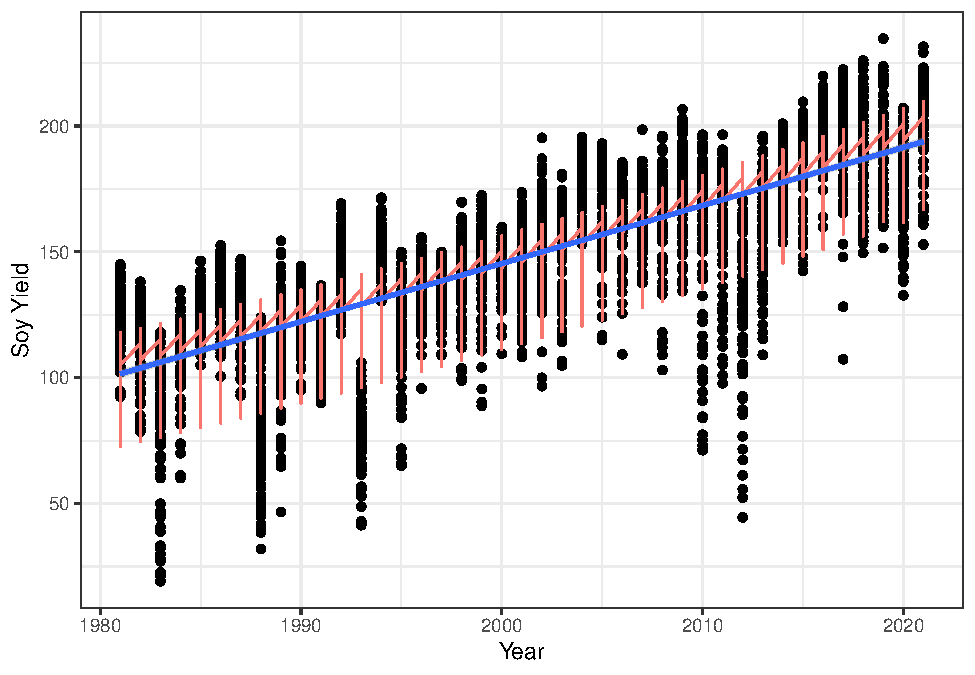
\includegraphics{Rportfolio-bookdown_files/figure-latex/unnamed-chunk-41-1.pdf}
\caption{\label{fig:unnamed-chunk-41}Soy yields over time (years) across all counties of Iowa, with a panel fit (orange), and linear fit (blue). Panel regression R squared is 0.660, with p\textless8.5e-06 for year and years squared versus yield.}
\end{figure}

Like with corn yields, soy yields in Iowa follow an upward trend over time, though with wide residuals (Figure 7).

\hypertarget{bonus-find-a-package-to-make-a-county-map-of-iowa-displaying-some-sort-of-information-about-yields-or-weather.-interpret-your-map.}{%
\section{Bonus: Find a package to make a county map of Iowa displaying some sort of information about yields or weather. Interpret your map.}\label{bonus-find-a-package-to-make-a-county-map-of-iowa-displaying-some-sort-of-information-about-yields-or-weather.-interpret-your-map.}}

\begin{Shaded}
\begin{Highlighting}[]
\FunctionTok{library}\NormalTok{(sf) }\CommentTok{\#Spatial package that can read and create shapefiles }
\FunctionTok{library}\NormalTok{(mapview) }\CommentTok{\#Interactive maps}
\FunctionTok{library}\NormalTok{(USAboundaries) }\CommentTok{\#USA states and counties}

\NormalTok{counties }\OtherTok{\textless{}{-}}\NormalTok{ us\_counties}

\NormalTok{Iowa\_ct }\OtherTok{\textless{}{-}} \FunctionTok{counties}\NormalTok{(}\AttributeTok{states =} \StringTok{\textquotesingle{}iowa\textquotesingle{}}\NormalTok{)}
\CommentTok{\#str(Iowa\_ct)}
\CommentTok{\#mapview(Iowa\_ct)}

\NormalTok{summer2018 }\OtherTok{\textless{}{-}}\NormalTok{ tmaxdf }\SpecialCharTok{\%\textgreater{}\%}
  \FunctionTok{filter}\NormalTok{(doy }\SpecialCharTok{\textgreater{}=} \DecValTok{152} \SpecialCharTok{\&}\NormalTok{ doy }\SpecialCharTok{\textless{}=} \DecValTok{243}\NormalTok{, year}\SpecialCharTok{==}\DecValTok{2018}\NormalTok{) }\SpecialCharTok{\%\textgreater{}\%} \CommentTok{\#day 152= June 1, 243= Aug 31}
  \FunctionTok{group\_by}\NormalTok{(countyfp, year) }\SpecialCharTok{\%\textgreater{}\%}
  \FunctionTok{summarize}\NormalTok{(}\AttributeTok{meantmax =} \FunctionTok{mean}\NormalTok{(tmax))}
\end{Highlighting}
\end{Shaded}

\begin{verbatim}
## `summarise()` has grouped output by 'countyfp'. You can override using the
## `.groups` argument.
\end{verbatim}

\begin{Shaded}
\begin{Highlighting}[]
\NormalTok{Itemp\_2018 }\OtherTok{\textless{}{-}} \FunctionTok{merge}\NormalTok{(Iowa\_ct, summer2018)}

\FunctionTok{mapview}\NormalTok{(Itemp\_2018, }\AttributeTok{zcol =}\StringTok{\textquotesingle{}meantmax\textquotesingle{}}\NormalTok{, }\AttributeTok{col.regions=}\FunctionTok{brewer.pal}\NormalTok{(}\DecValTok{9}\NormalTok{, }\StringTok{"OrRd"}\NormalTok{), }\AttributeTok{layer.name =} \StringTok{"Mean Max. Summer Temp. (C)"}\NormalTok{)}
\end{Highlighting}
\end{Shaded}


  \bibliography{packages.bib}

\end{document}
